\documentclass[compress]{beamer}
\usepackage{ifthen,verbatim,algorithmic}

\newcommand{\isnote}{}
\xdefinecolor{lightyellow}{rgb}{1.,1.,0.25}
\xdefinecolor{darkblue}{rgb}{0.1,0.1,0.7}
\xdefinecolor{darkgreen}{rgb}{0.0,0.5,0.0}
\xdefinecolor{purple}{rgb}{0.7,0.1,0.7}

%% Uncomment this to get annotations
%% \def\notes{\addtocounter{page}{-1}
%%            \renewcommand{\isnote}{*}
%% 	   \beamertemplateshadingbackground{lightyellow}{white}
%%            \begin{frame}
%%            \frametitle{Notes for the previous page (page \insertpagenumber)}
%%            \itemize}
%% \def\endnotes{\enditemize
%% 	      \end{frame}
%%               \beamertemplateshadingbackground{white}{white}
%%               \renewcommand{\isnote}{}}

%% Uncomment this to not get annotations
\def\notes{\comment}
\def\endnotes{\endcomment}

\setbeamertemplate{navigation symbols}{}
\setbeamertemplate{headline}{\mbox{ } \hfill
\begin{minipage}{5.5 cm}
\vspace{-0.75 cm} \small
\end{minipage} \hfill
\begin{minipage}{4.5 cm}
\vspace{-0.75 cm} \small
\begin{flushright}
\ifthenelse{\equal{\insertpagenumber}{1}}{}{Jim Pivarski \hspace{0.2 cm} \insertpagenumber\isnote/\pageref{numpages}}
\end{flushright}
\end{minipage}\mbox{\hspace{0.2 cm}}\includegraphics[height=1 cm]{../cmslogo} \hspace{0.1 cm} \includegraphics[height=1 cm]{../tamulogo} \hspace{0.01 cm} \vspace{-1.05 cm}}

\newcommand{\s}[1]{{\mbox{\scriptsize #1}}}

\begin{document}
\begin{frame}
\vfill
\begin{center}
\textcolor{darkblue}{\Large Study of TrackerMuon Residuals}

\vfill
\begin{columns}
\column{0.3\linewidth}
\begin{center}
\large
Jim Pivarski
\end{center}
\end{columns}

\begin{columns}
\column{0.3\linewidth}
\begin{center}
\scriptsize
{\it Texas A\&M University}
\end{center}
\end{columns}

\vfill
 3 September, 2010

\end{center}
\end{frame}

%% \begin{notes}
%% \item This is the annotated version of my talk.
%% \item If you want the version that I am presenting, download the one
%% labeled ``slides'' on Indico (or just ignore these yellow pages).
%% \item The annotated version is provided for extra detail and a written
%% record of comments that I intend to make orally.
%% \item Yellow notes refer to the content on the {\it previous} page.
%% \item All other slides are identical for the two versions.
%% \end{notes}

\small

\begin{frame}
\frametitle{Avoid trigger bias}
\begin{itemize}
\item Since triggers are tighter in collisions data than they are in
  cosmics, it is important to make sure that the trigger requirements
  are not sculpting the muon distributions
\item The method I used in this study:

\begin{algorithmic}
\STATE \textcolor{darkgreen}{trigger} = HLT\_Mu9 (lowest unprescaled single-$\mu$ trigger)
\STATE \textcolor{darkgreen}{triggerable muon} = muon with $p_T > 11$~GeV/$c$, $|\eta| < 2.1$

\vspace{0.2 cm}
\IF {\textcolor{black}{passed trigger} \AND \textcolor{black}{number of triggerable muons} $>$ 0}
\FOR {loop over muons}
\IF {\textcolor{black}{number of triggerable muons} = 1 \AND this muon isn't it}
\STATE \textcolor{darkblue}{include this muon in plots!} (case 1)
\ELSIF {\textcolor{black}{number of triggerable muons} $>$ 1}
\STATE \textcolor{darkblue}{include this muon in plots!} (case 2)
\ENDIF
\ENDFOR
\ENDIF
\end{algorithmic}

\item Every event we look at has at least two muons in it
\end{itemize}
\end{frame}

\begin{frame}
\frametitle{Residuals per ring of chambers}
\begin{itemize}
\item Not enough statistics to bin residuals by chamber

\item Bin by rings of identical chambers
\begin{itemize}
\item barrel wheels 0, $\pm$1, $\pm$2 in stations 1, 2, 3, 4
\item endcap stations 1/1, 1/2, 1/3, 2/1, 2/2, 3/1, 3/2, 4/1, 4/2
\end{itemize}

\item Additionally require the muons to share a vertex with
  $P_\s{vertex} > 1\%$ (reduces backgrounds from decays-in-flight)

\item Muons are mostly from double-semileptonic decays ($b \to c \to
  s$ with both $W \to \mu\nu$) and dimuon resonances ($J/\psi$)

\item Re-fit PromptReco with the latest alignment in 3\_8\_2

\item Examples (points are data, shaded blue/grey is Monte Carlo):
\end{itemize}

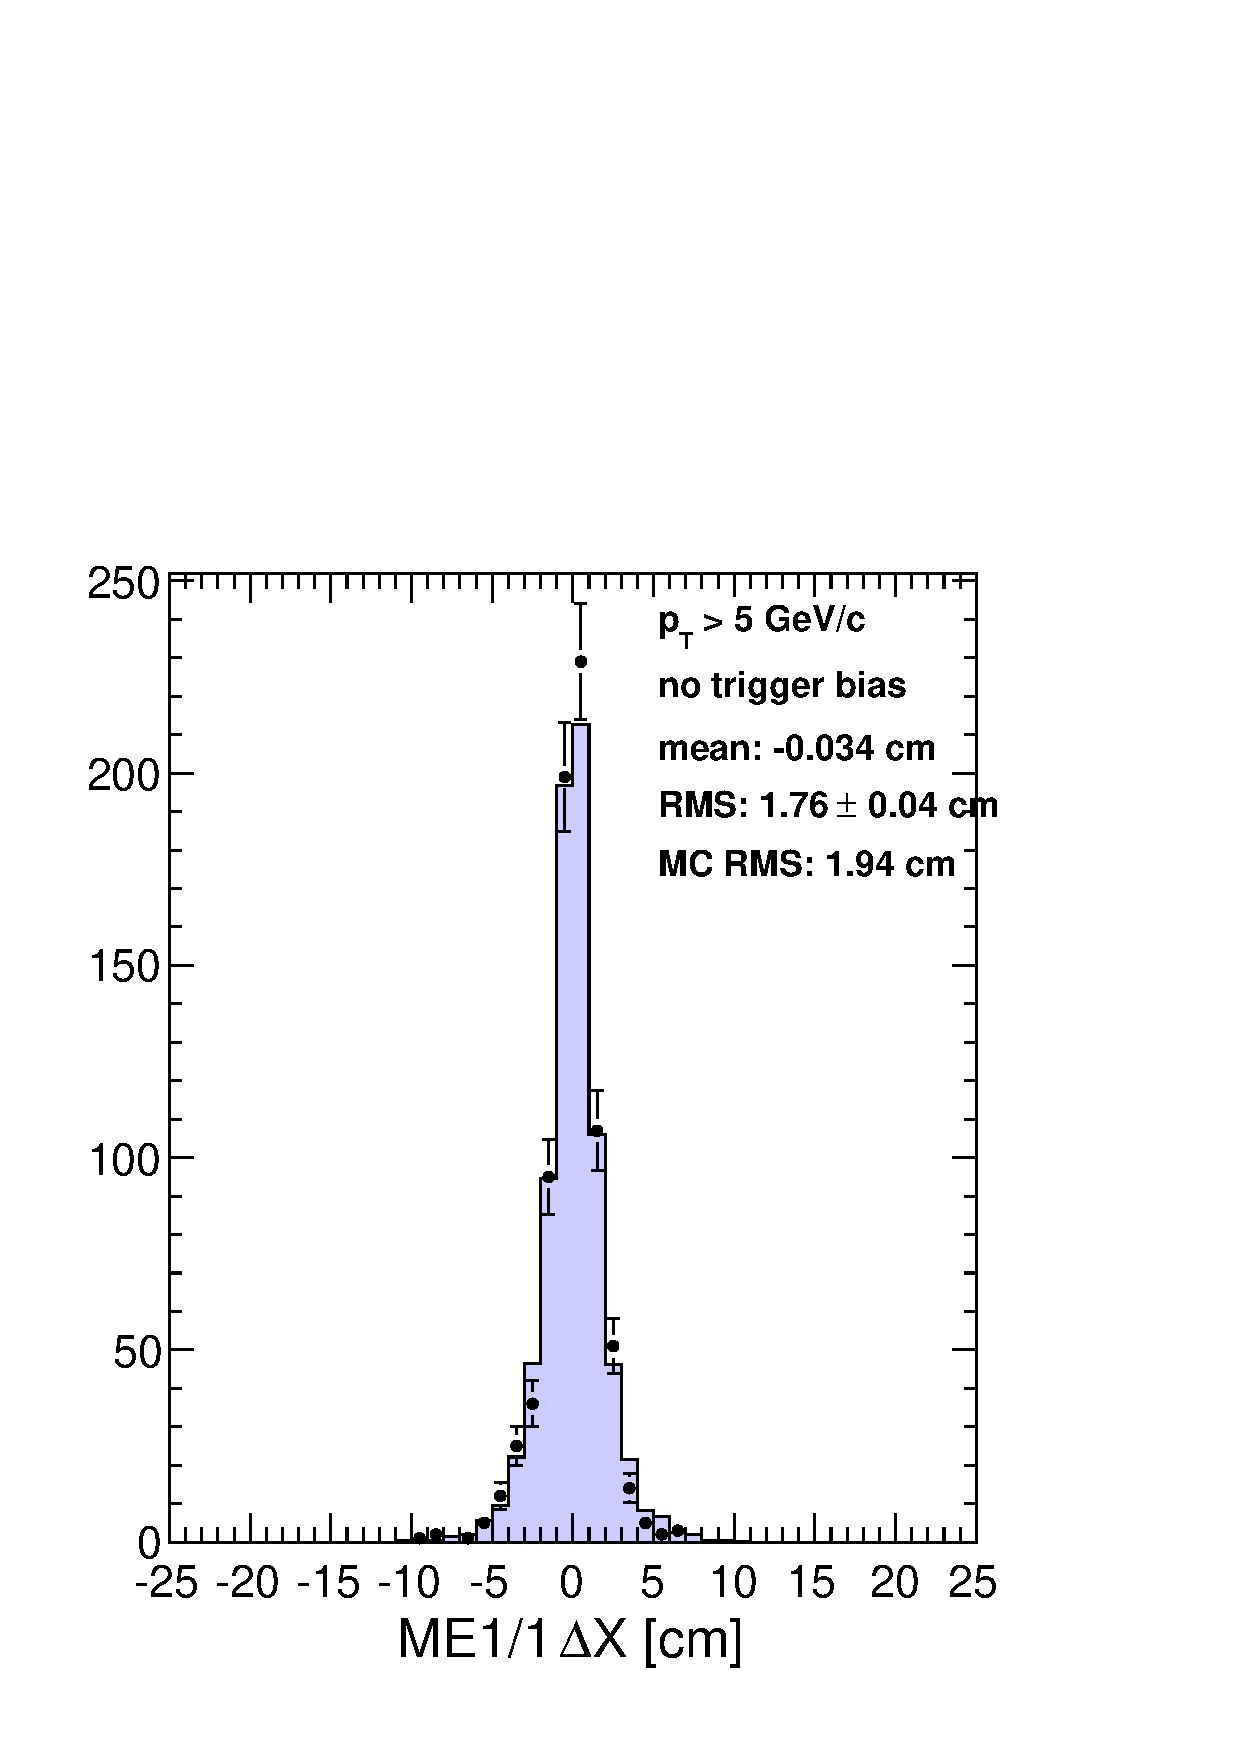
\includegraphics[width=0.24\linewidth]{me11_X.pdf}
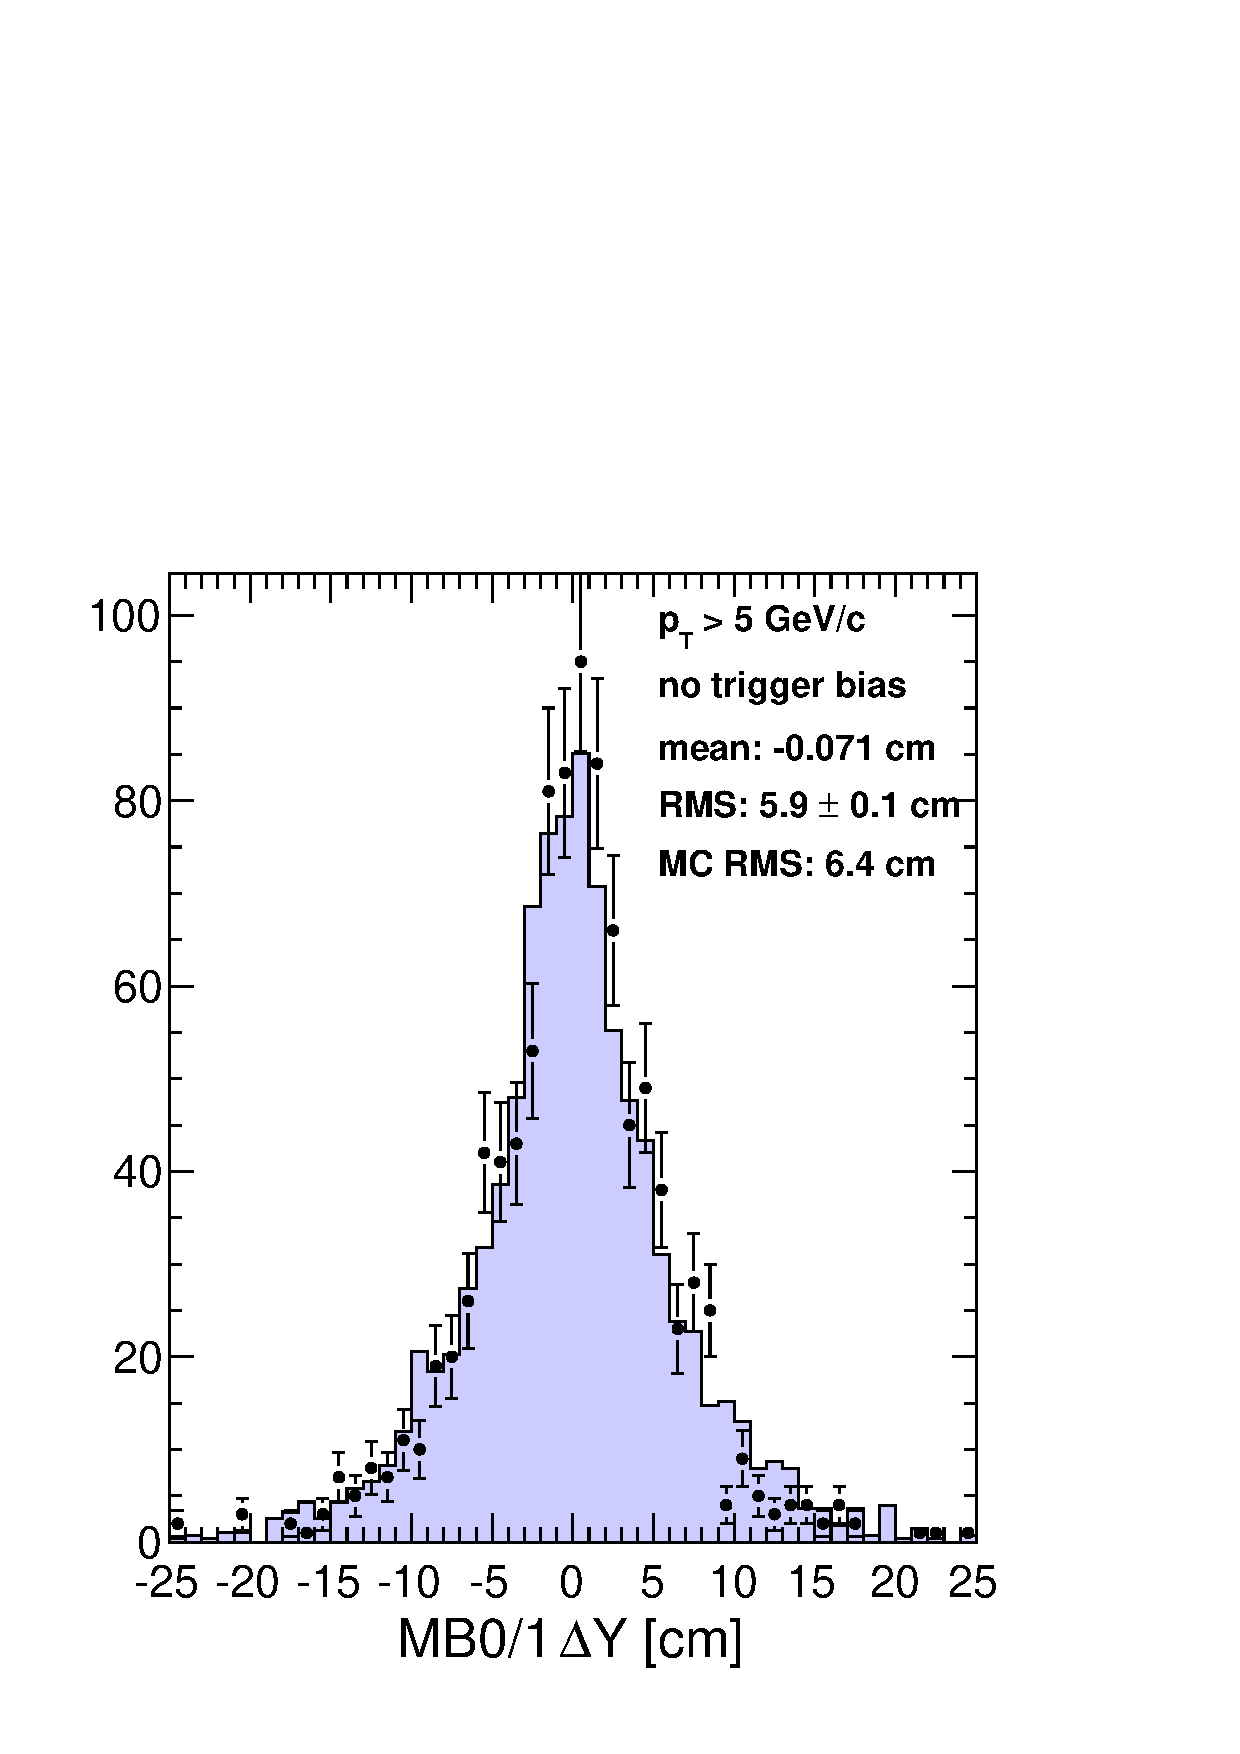
\includegraphics[width=0.24\linewidth]{mb01_Y.pdf}
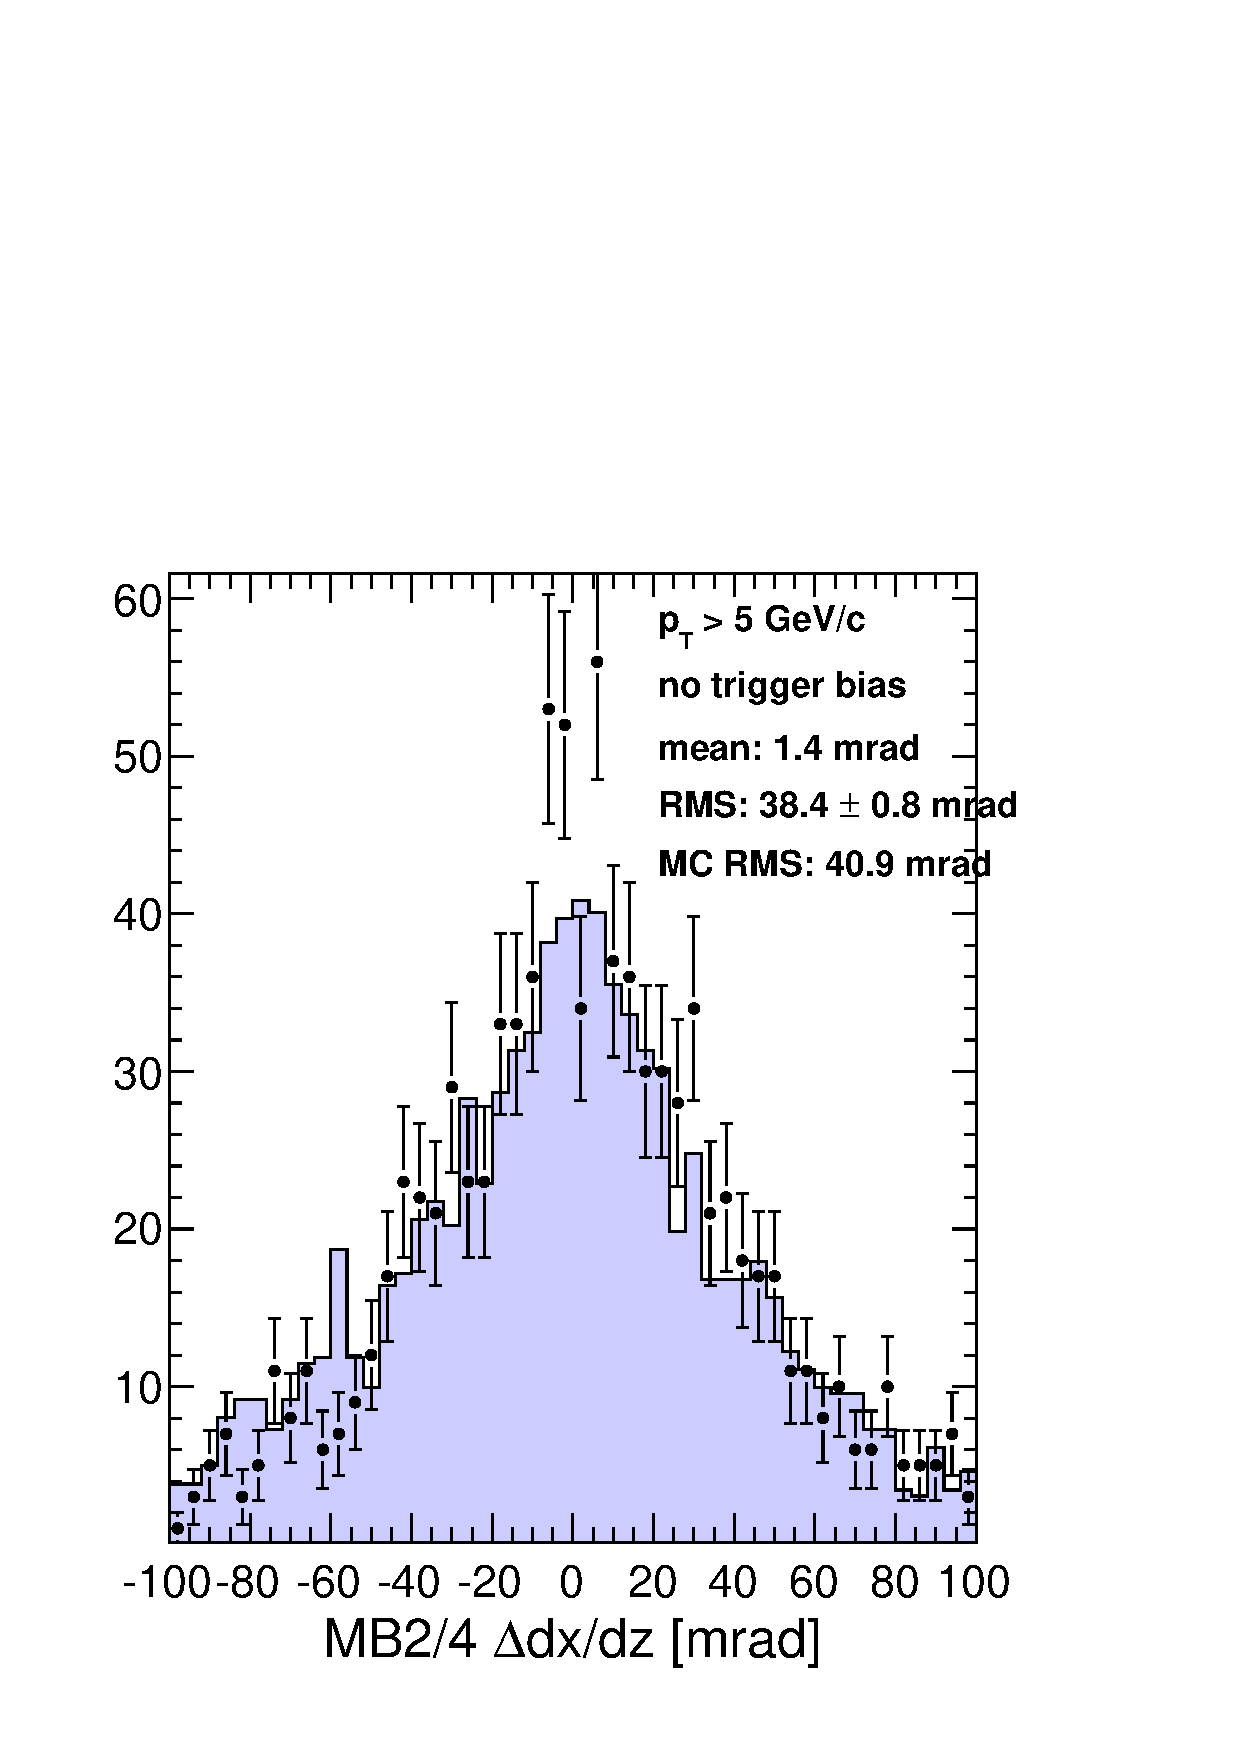
\includegraphics[width=0.24\linewidth]{mb24_dXdZ.pdf}
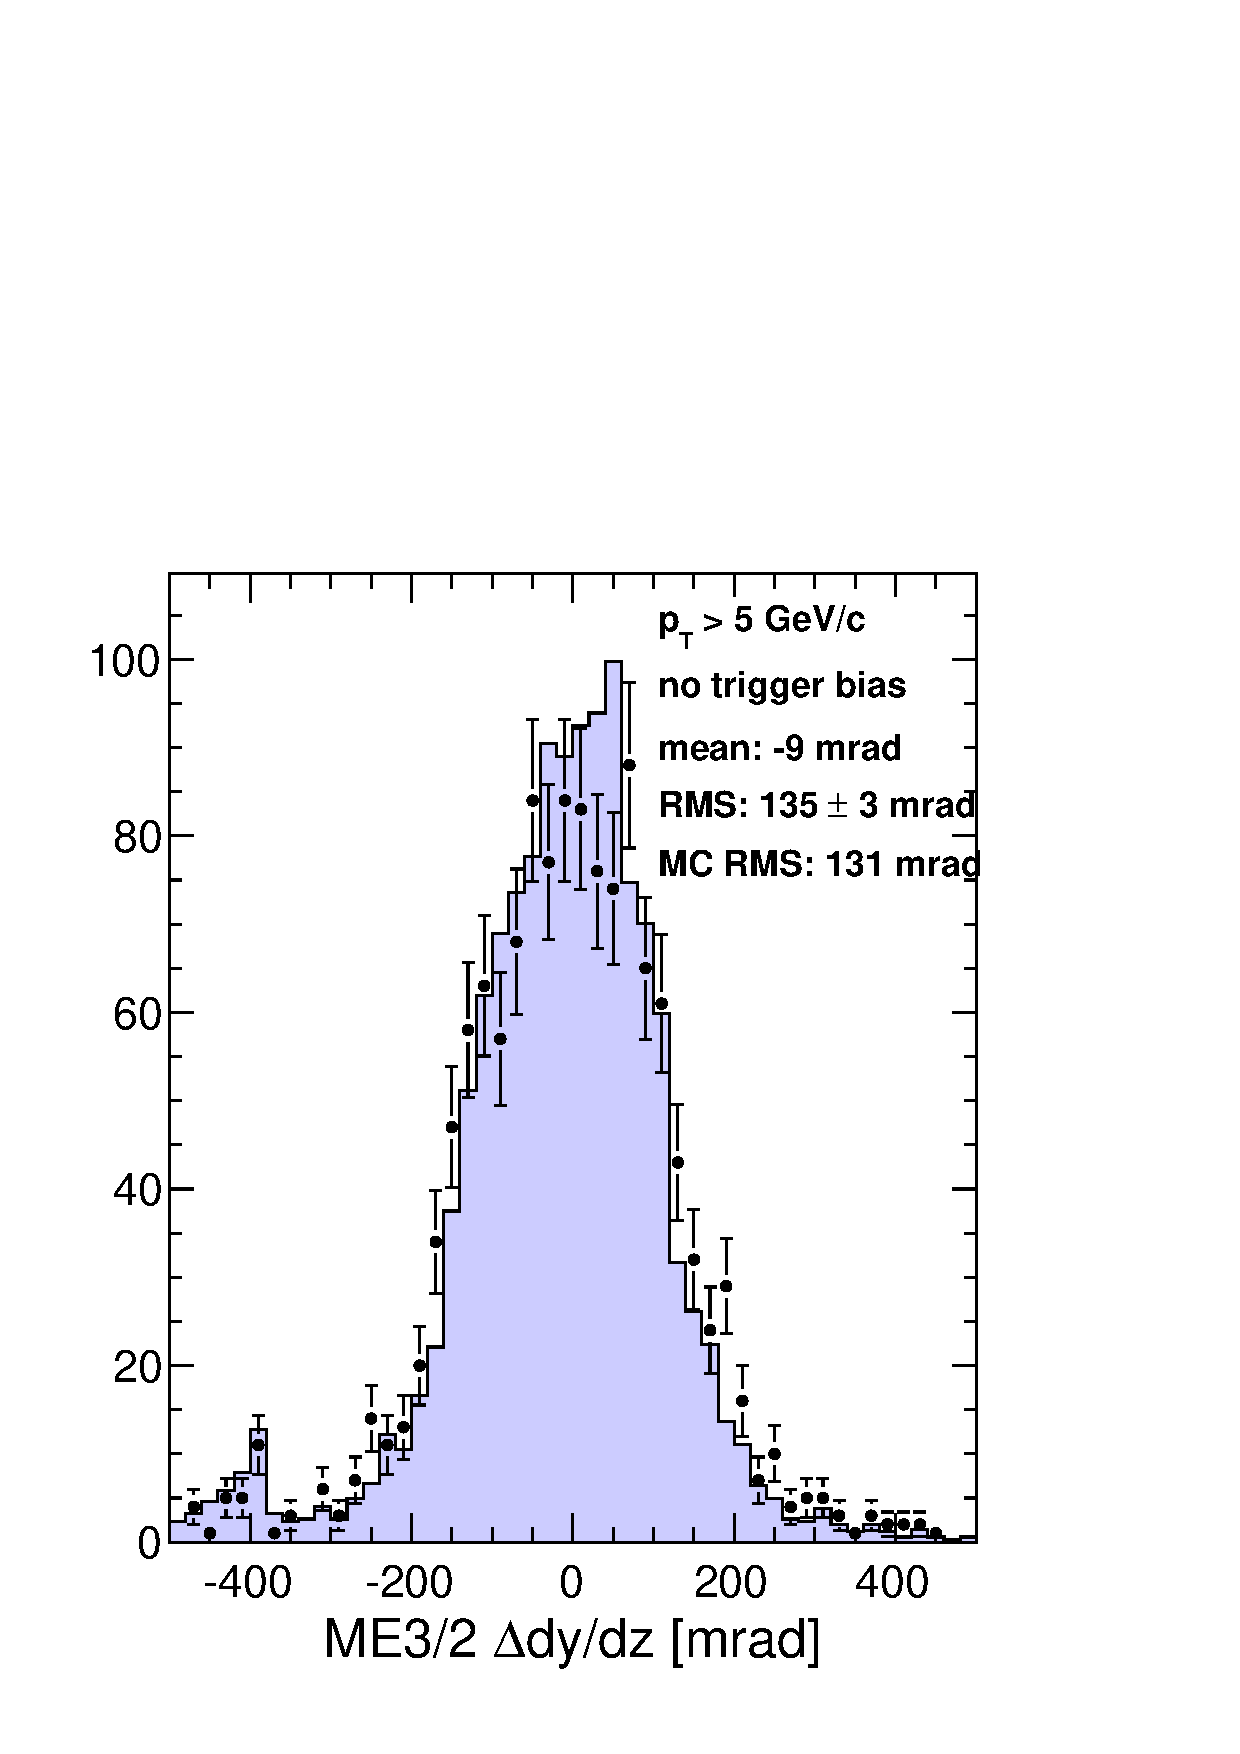
\includegraphics[width=0.24\linewidth]{me32_dYdZ.pdf}
\end{frame}

\begin{frame}
\frametitle{Summary plots}

\begin{itemize}
\item MC is a little wider than the data everywhere
\item MC has STARTUP conditions re-tracked with IDEAL alignment: could
  be the influence of mis{\it calibrated} hits?
\end{itemize}
\begin{center}
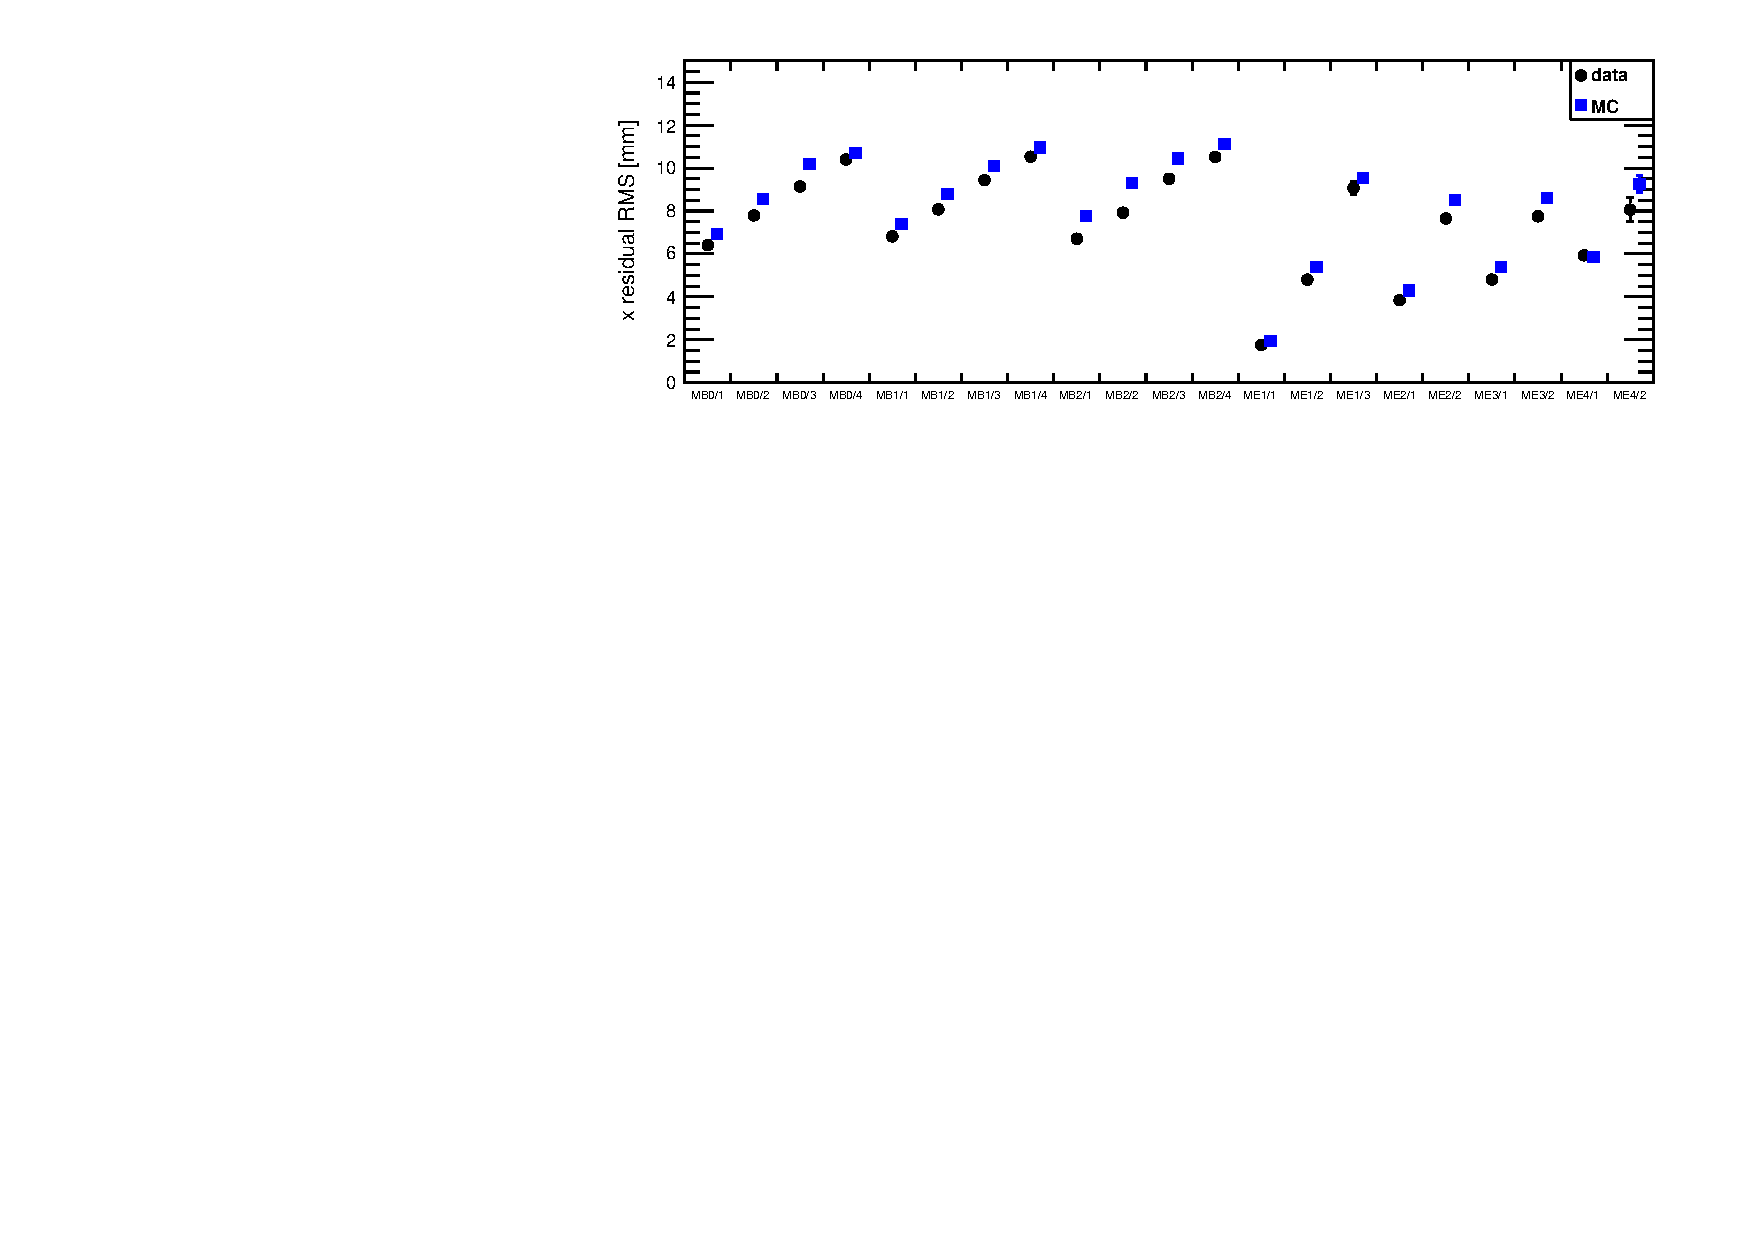
\includegraphics[width=0.9\linewidth]{summaryX.pdf}

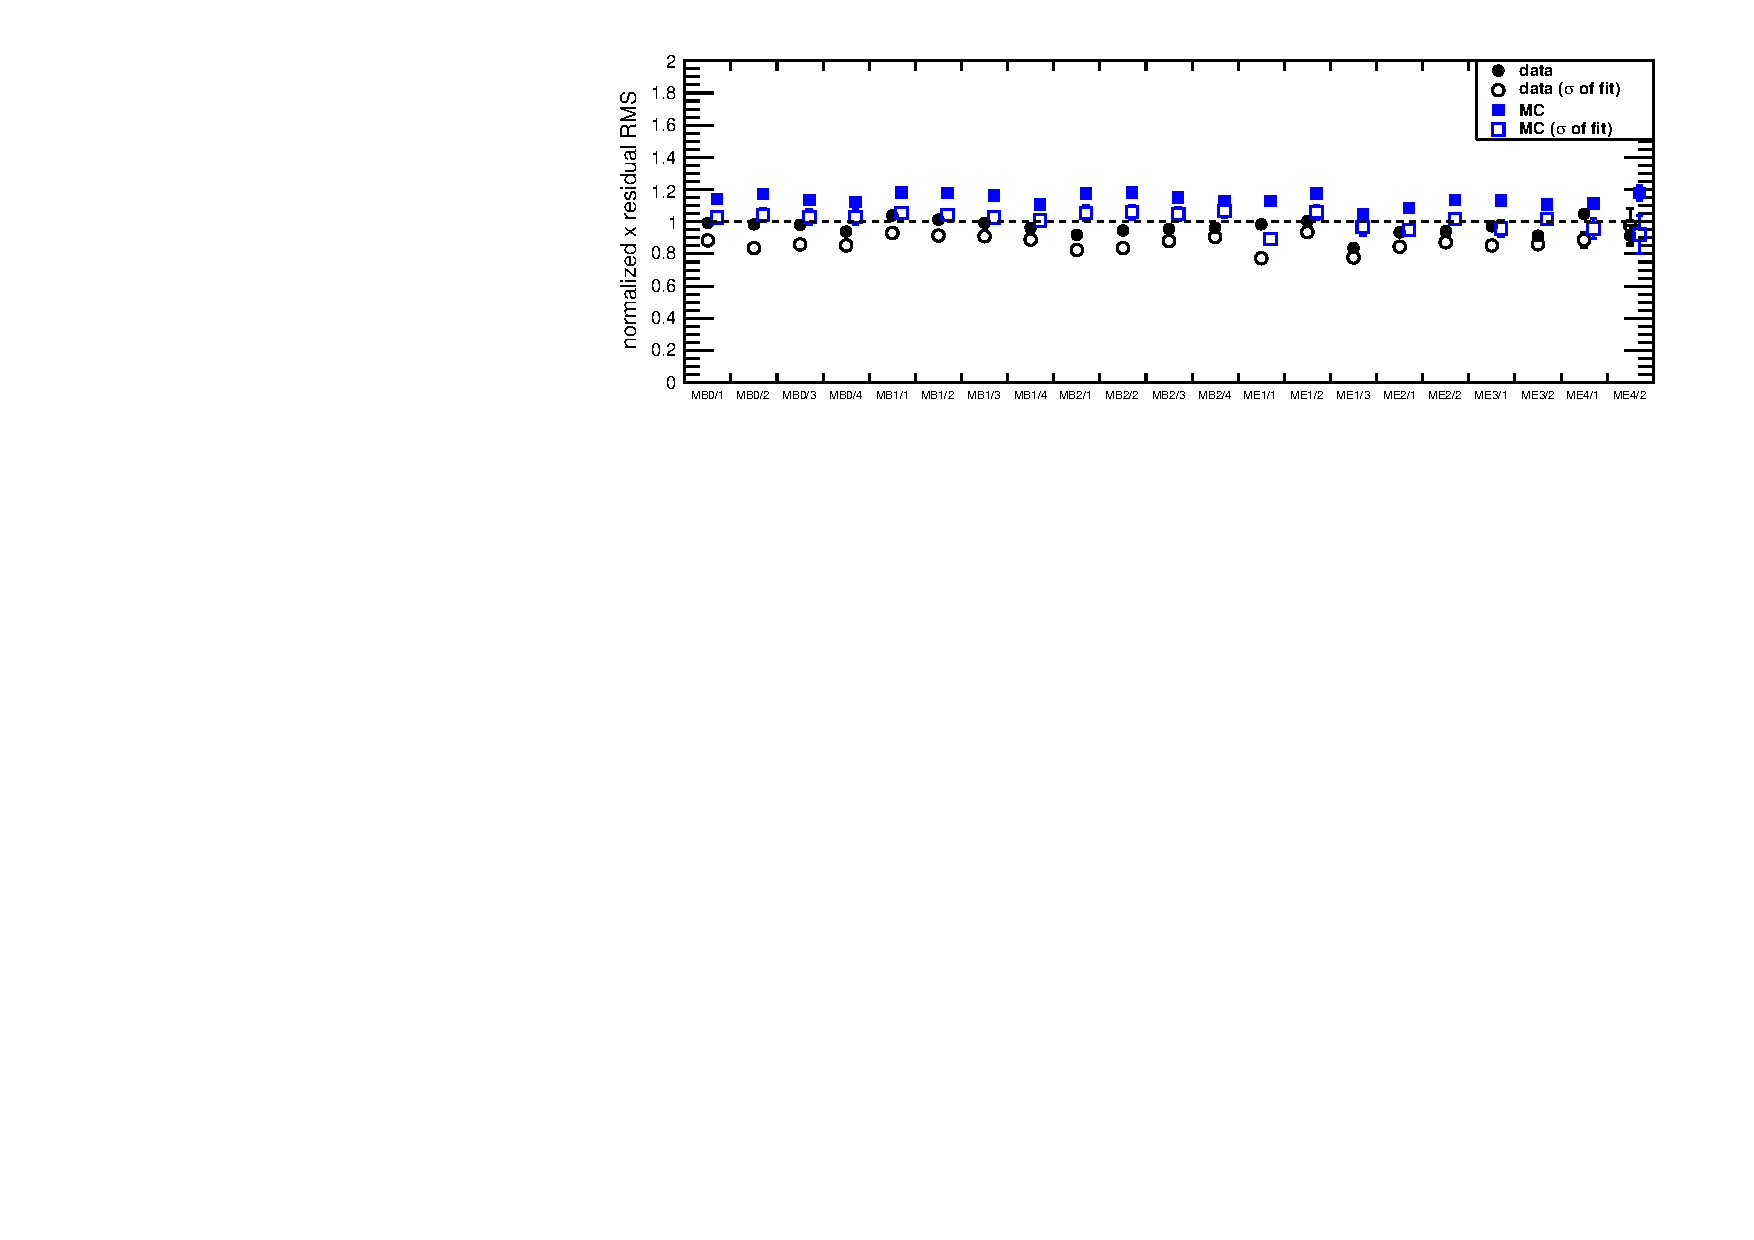
\includegraphics[width=0.9\linewidth]{summaryXnorm.pdf}
\end{center}
\end{frame}

\begin{frame}
\frametitle{Summary plots}

\begin{itemize}
\item Same for $y$
\item Compared with standard RelVals (similar results):
\href{http://cmsdoc.cern.ch/cms/Physics/muon/CMSSW/Performance/RecoMuon/MuonIdentification/}{\textcolor{blue}{\tt \tiny http://cmsdoc.cern.ch/cms/Physics/muon/CMSSW/Performance/RecoMuon/MuonIdentification/}}
\end{itemize}
\begin{center}
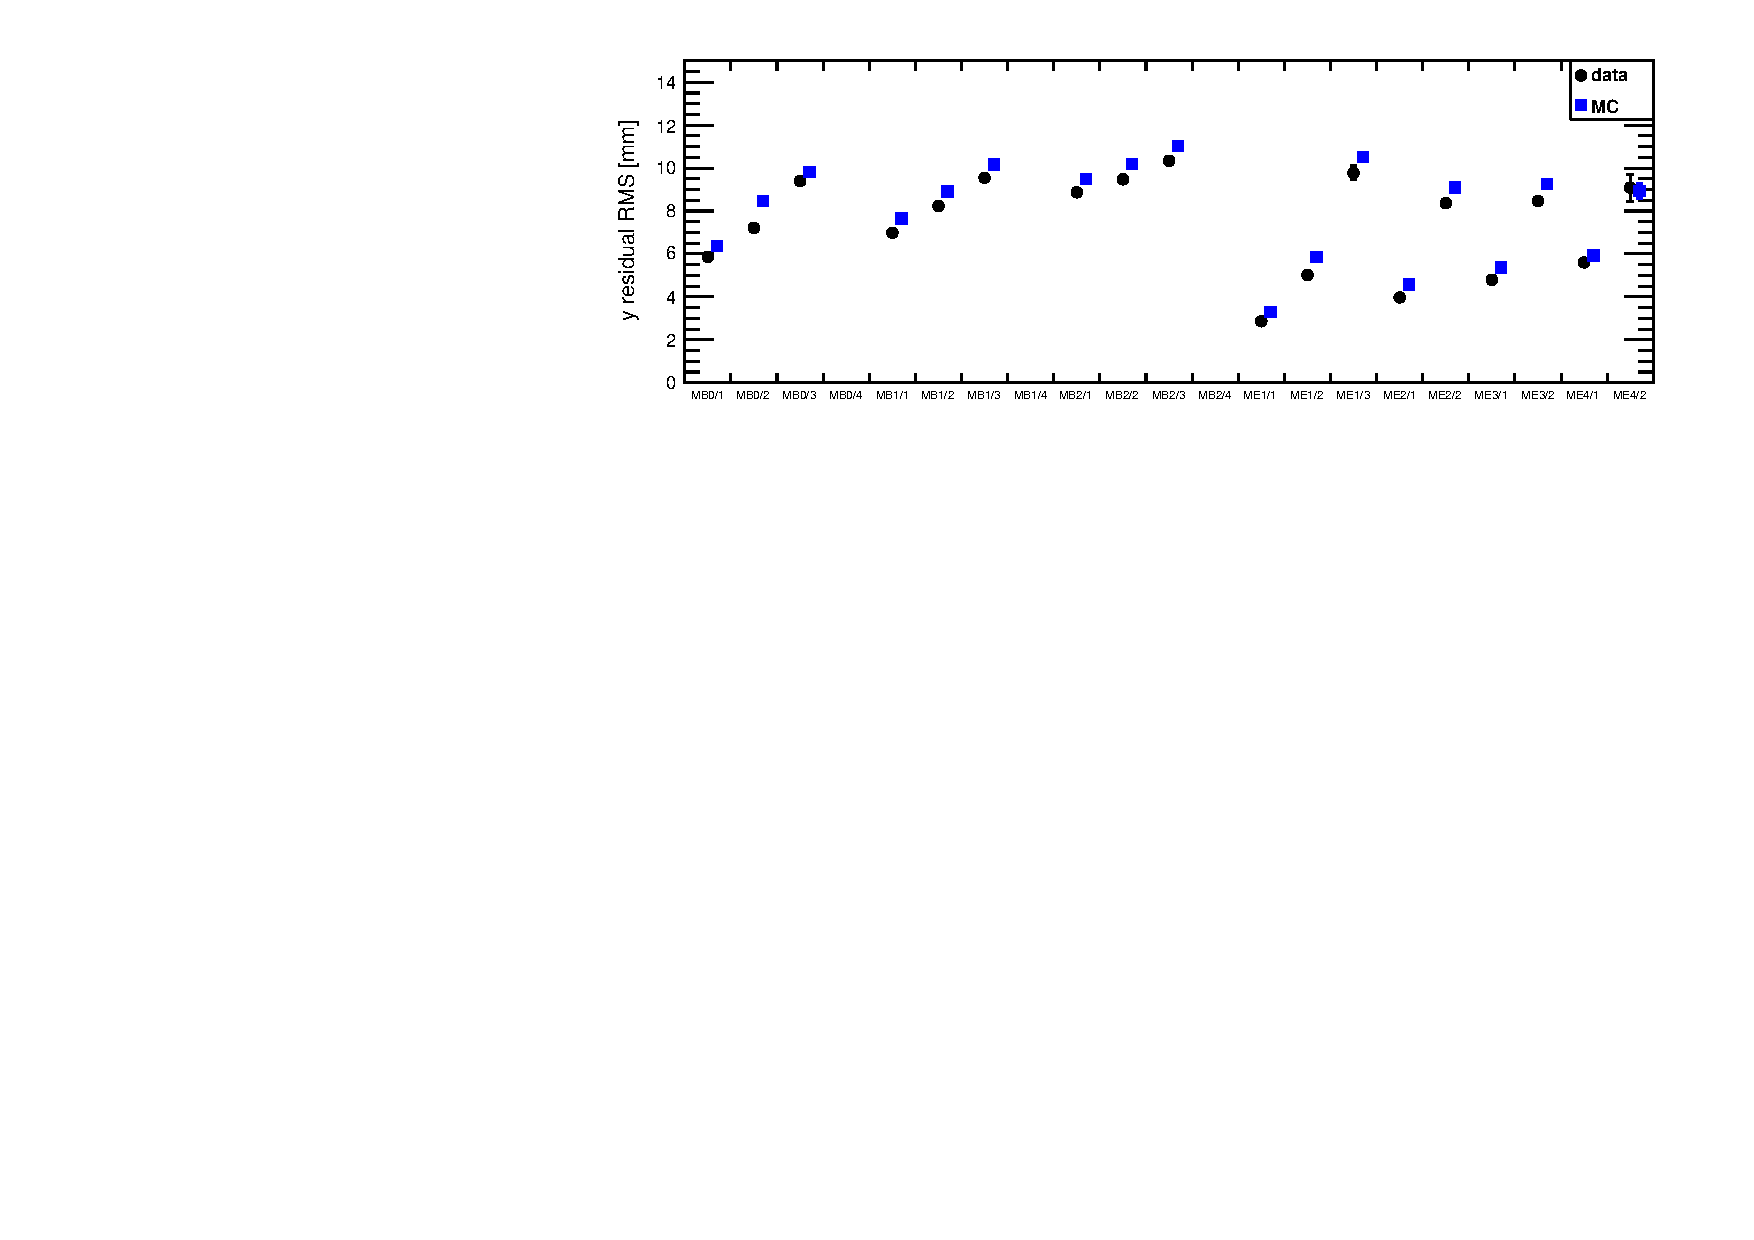
\includegraphics[width=0.9\linewidth]{summaryY.pdf}

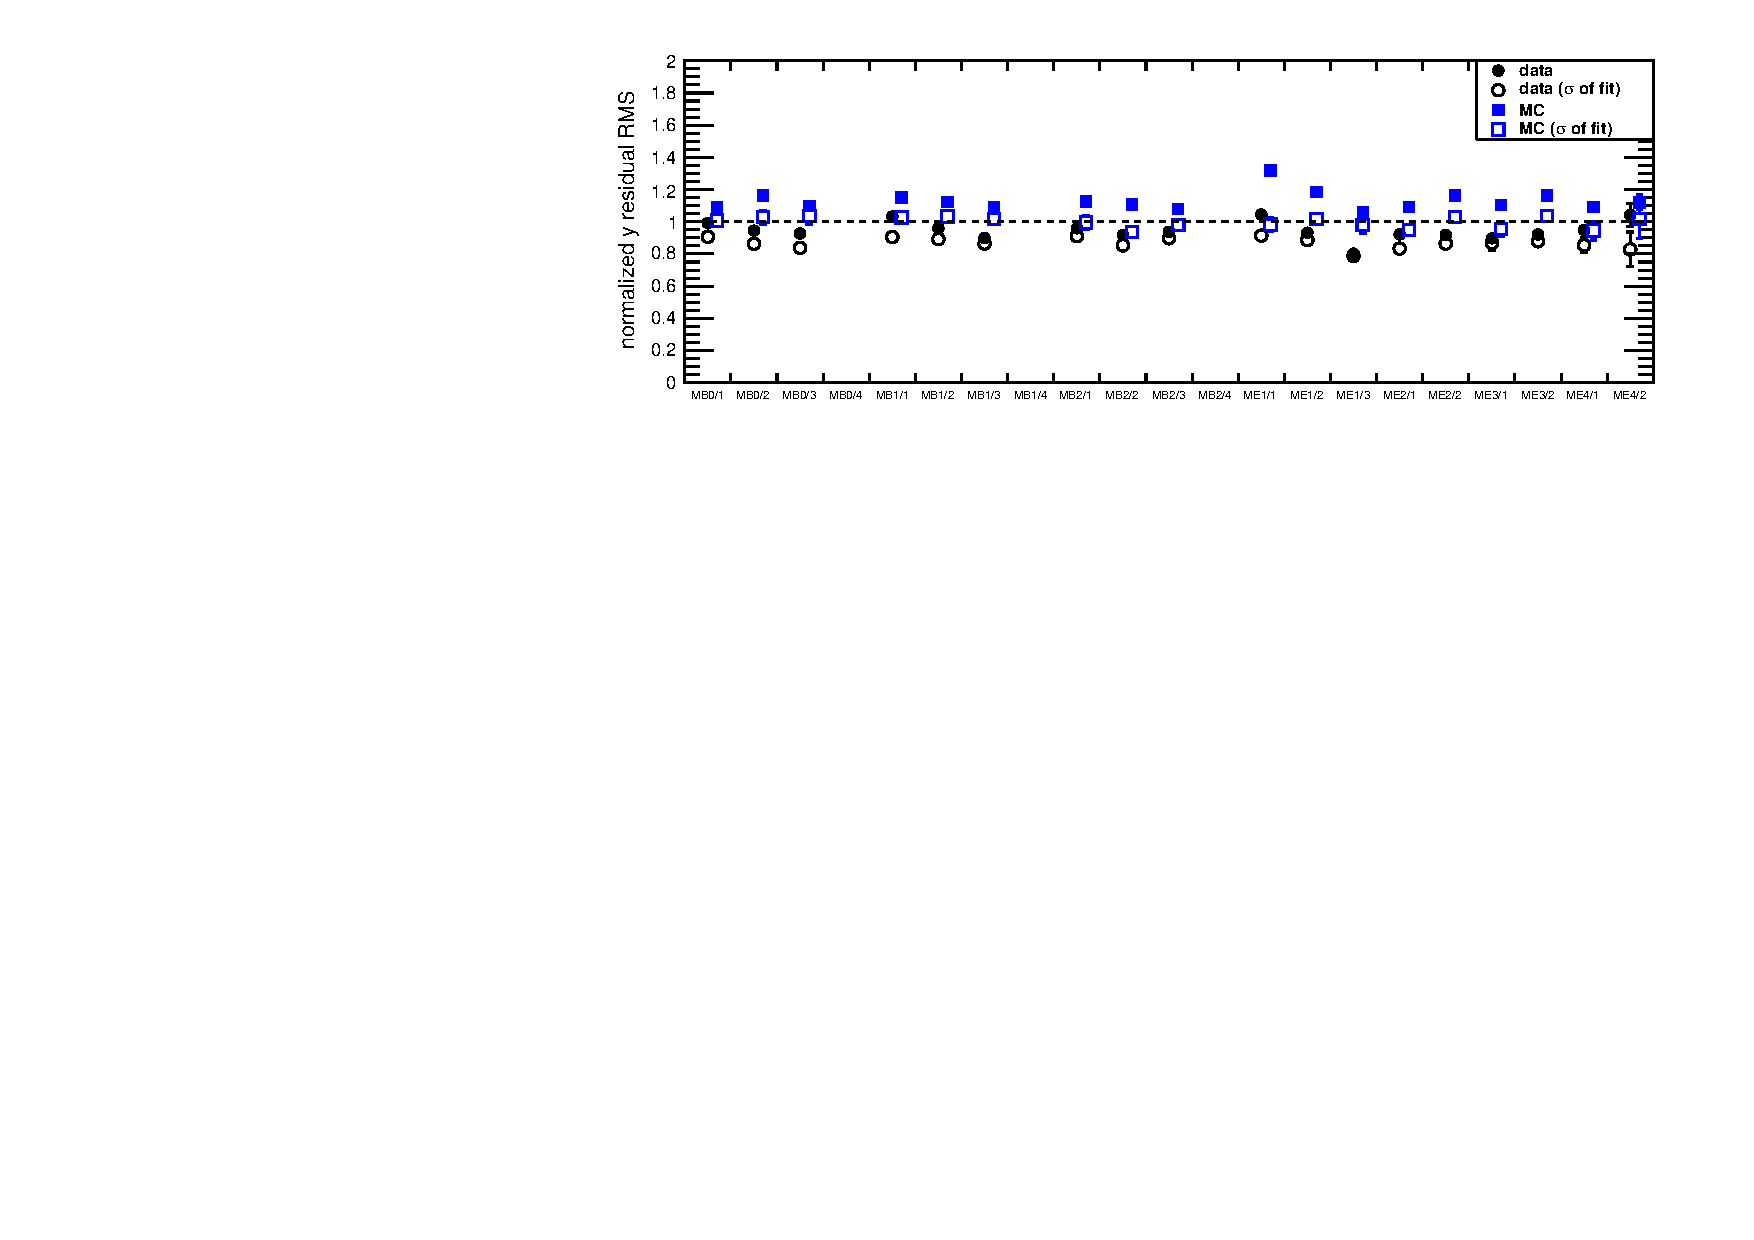
\includegraphics[width=0.9\linewidth]{summaryYnorm.pdf}
\end{center}
\end{frame}

\begin{frame}
\frametitle{Summary plots}

\begin{itemize}
\item Endcap normalized $\Delta \frac{dx}{dz}$ distributions have tails (RMS $>$ $\sigma$)
\item $\delta_{\phi_y}$ (directly related to $\Delta \frac{dx}{dz}$) has not been aligned in the endcap
\item But this pattern is reproduced in MC--- doesn't seem like misalignment is the problem
\end{itemize}
\begin{columns}
\column{0.8\linewidth}
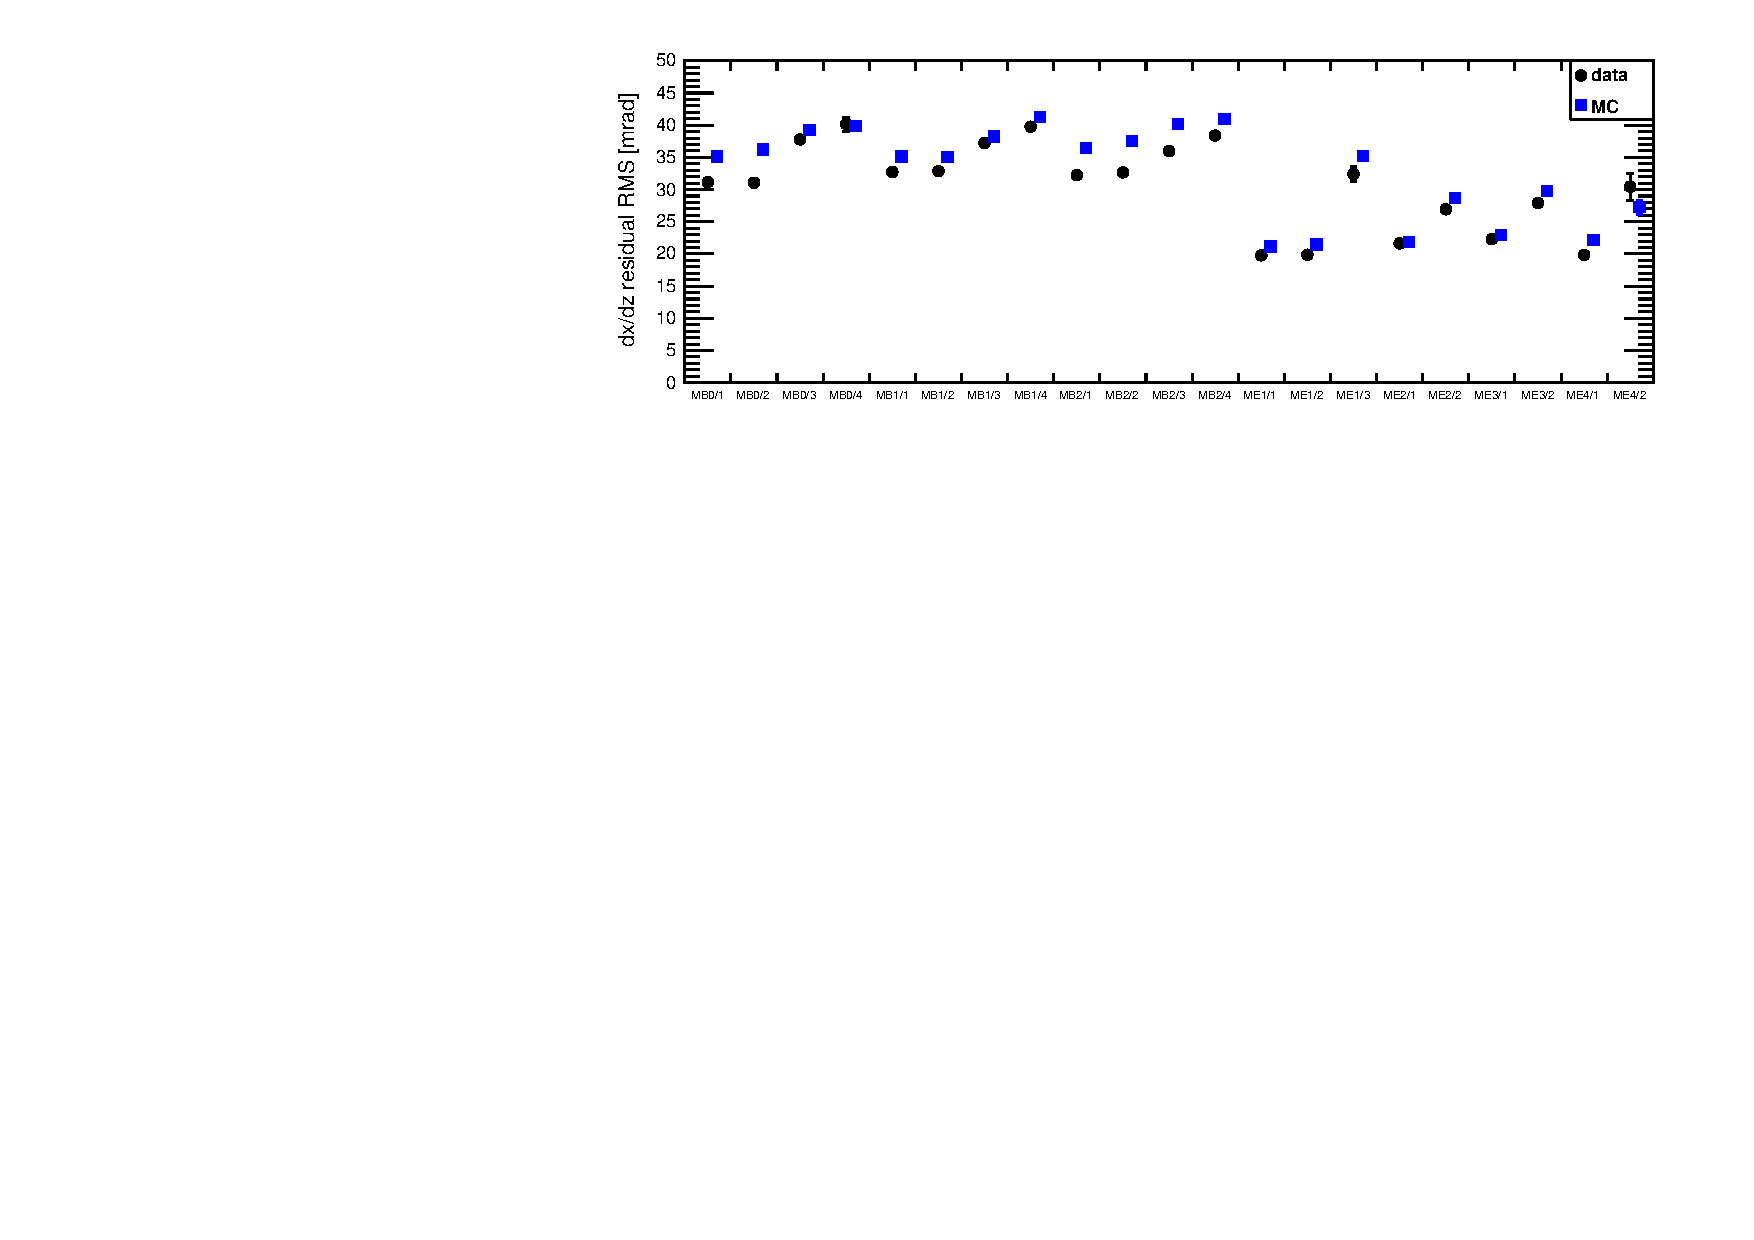
\includegraphics[width=\linewidth]{summarydXdZ.pdf}

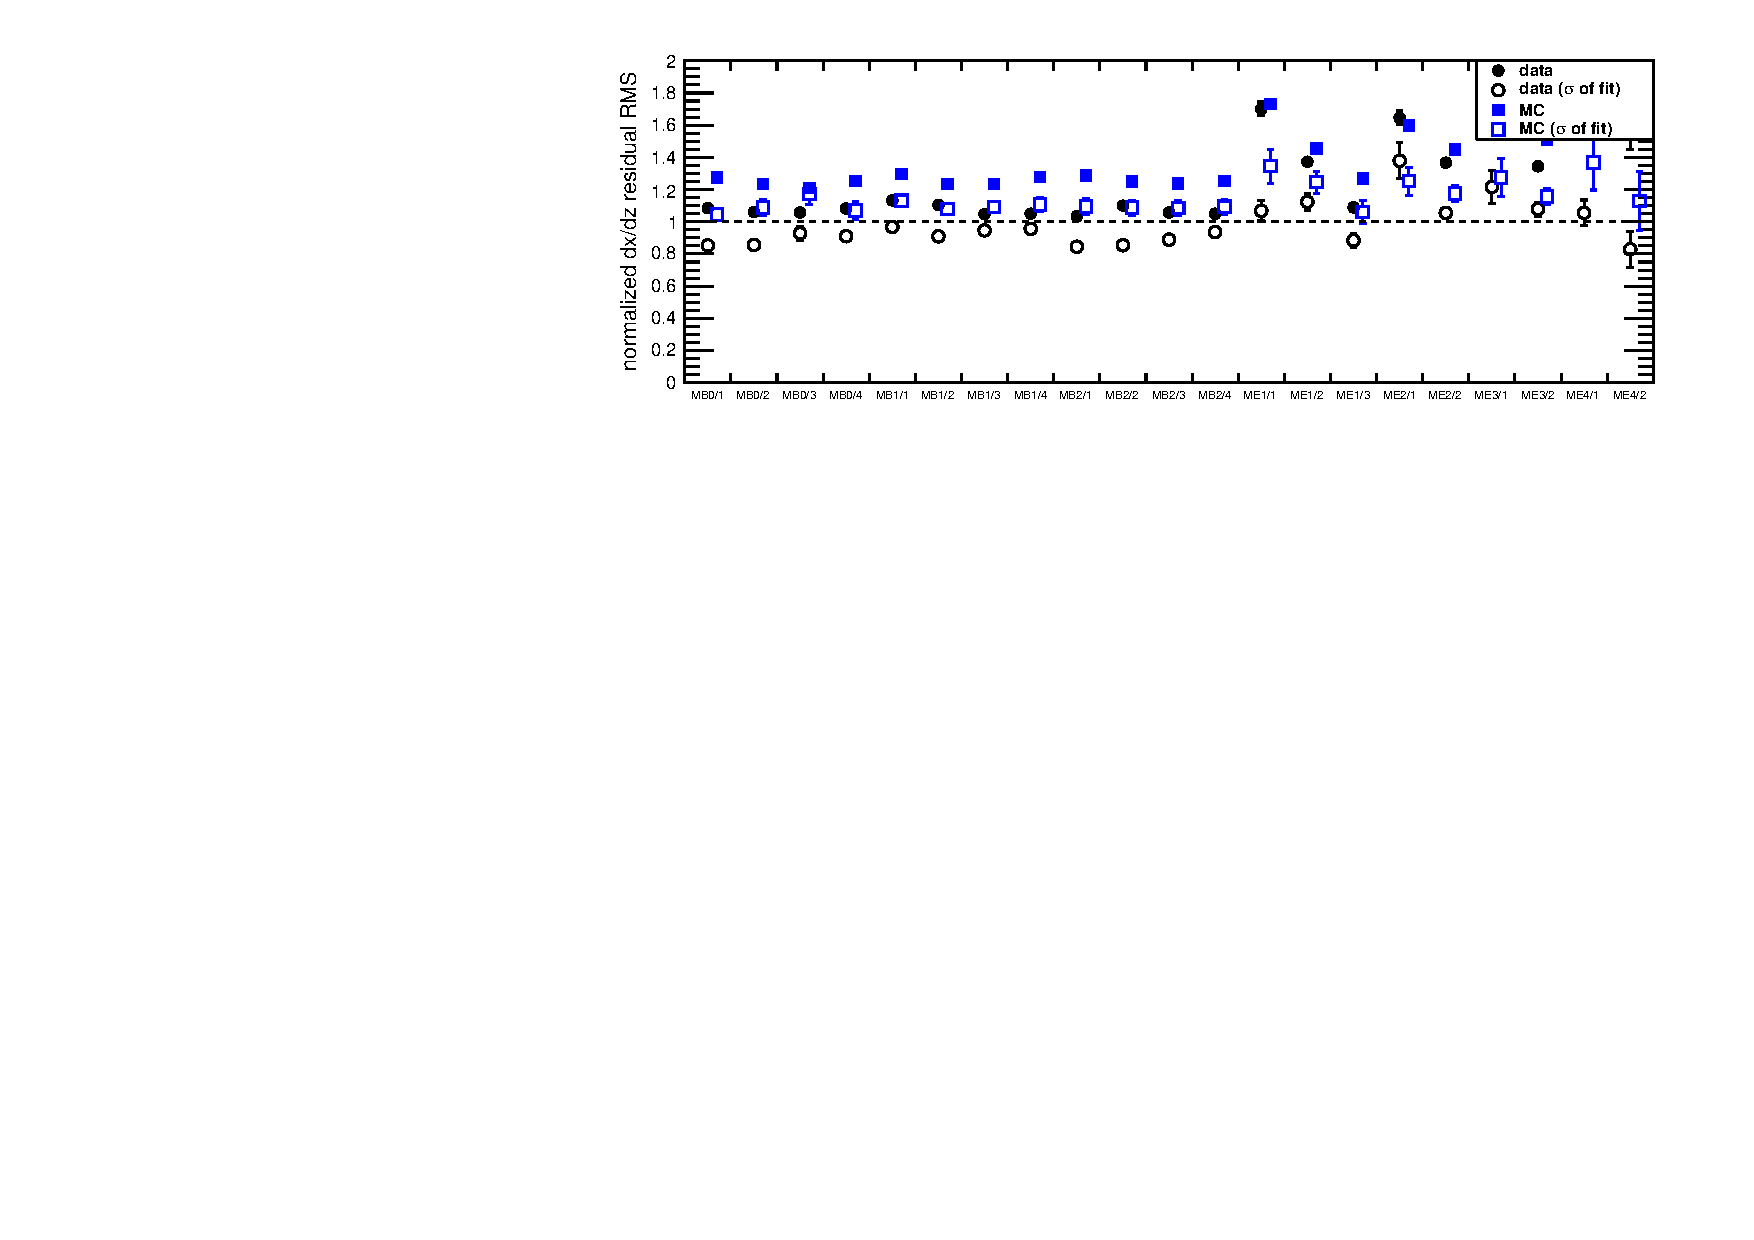
\includegraphics[width=\linewidth]{summarydXdZnorm.pdf}

\column{0.2\linewidth}
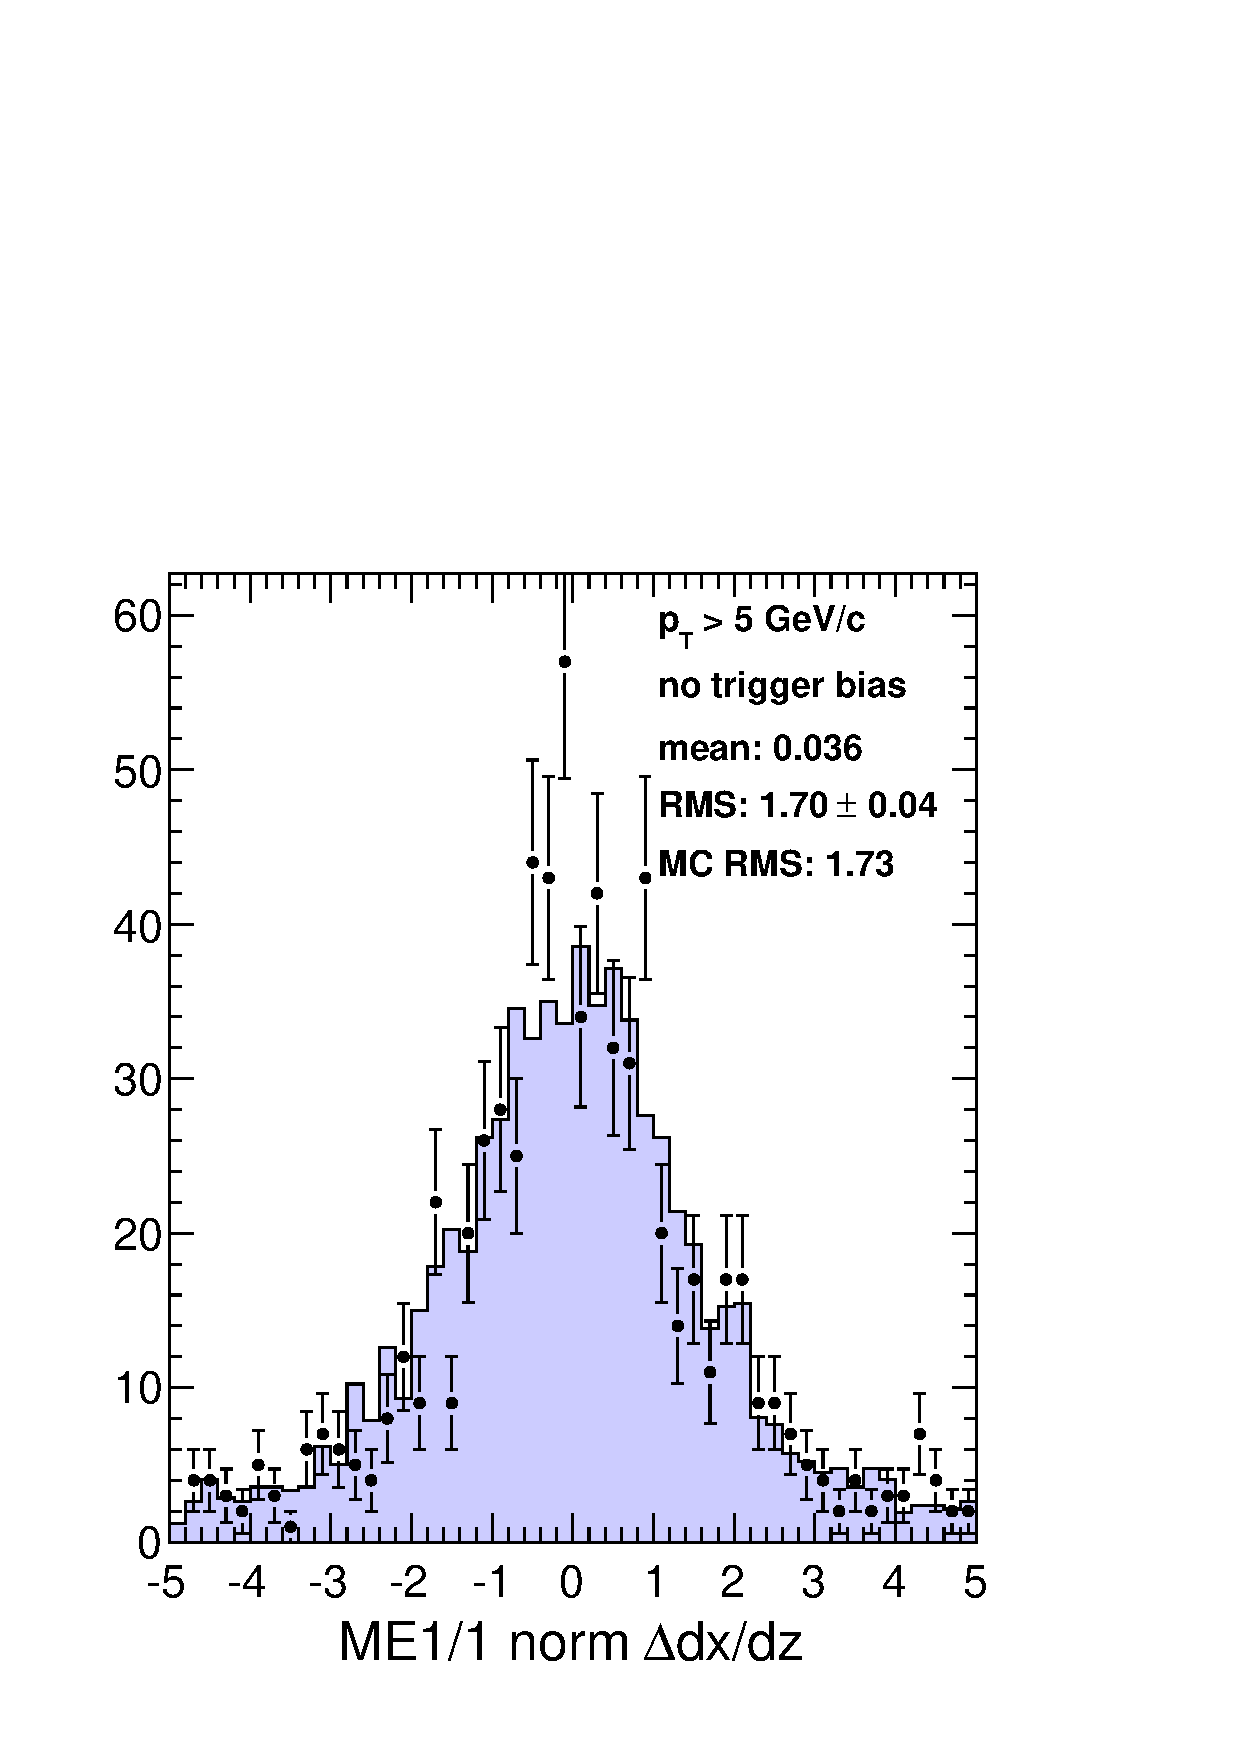
\includegraphics[width=\linewidth]{me11_dXdZnorm.pdf}

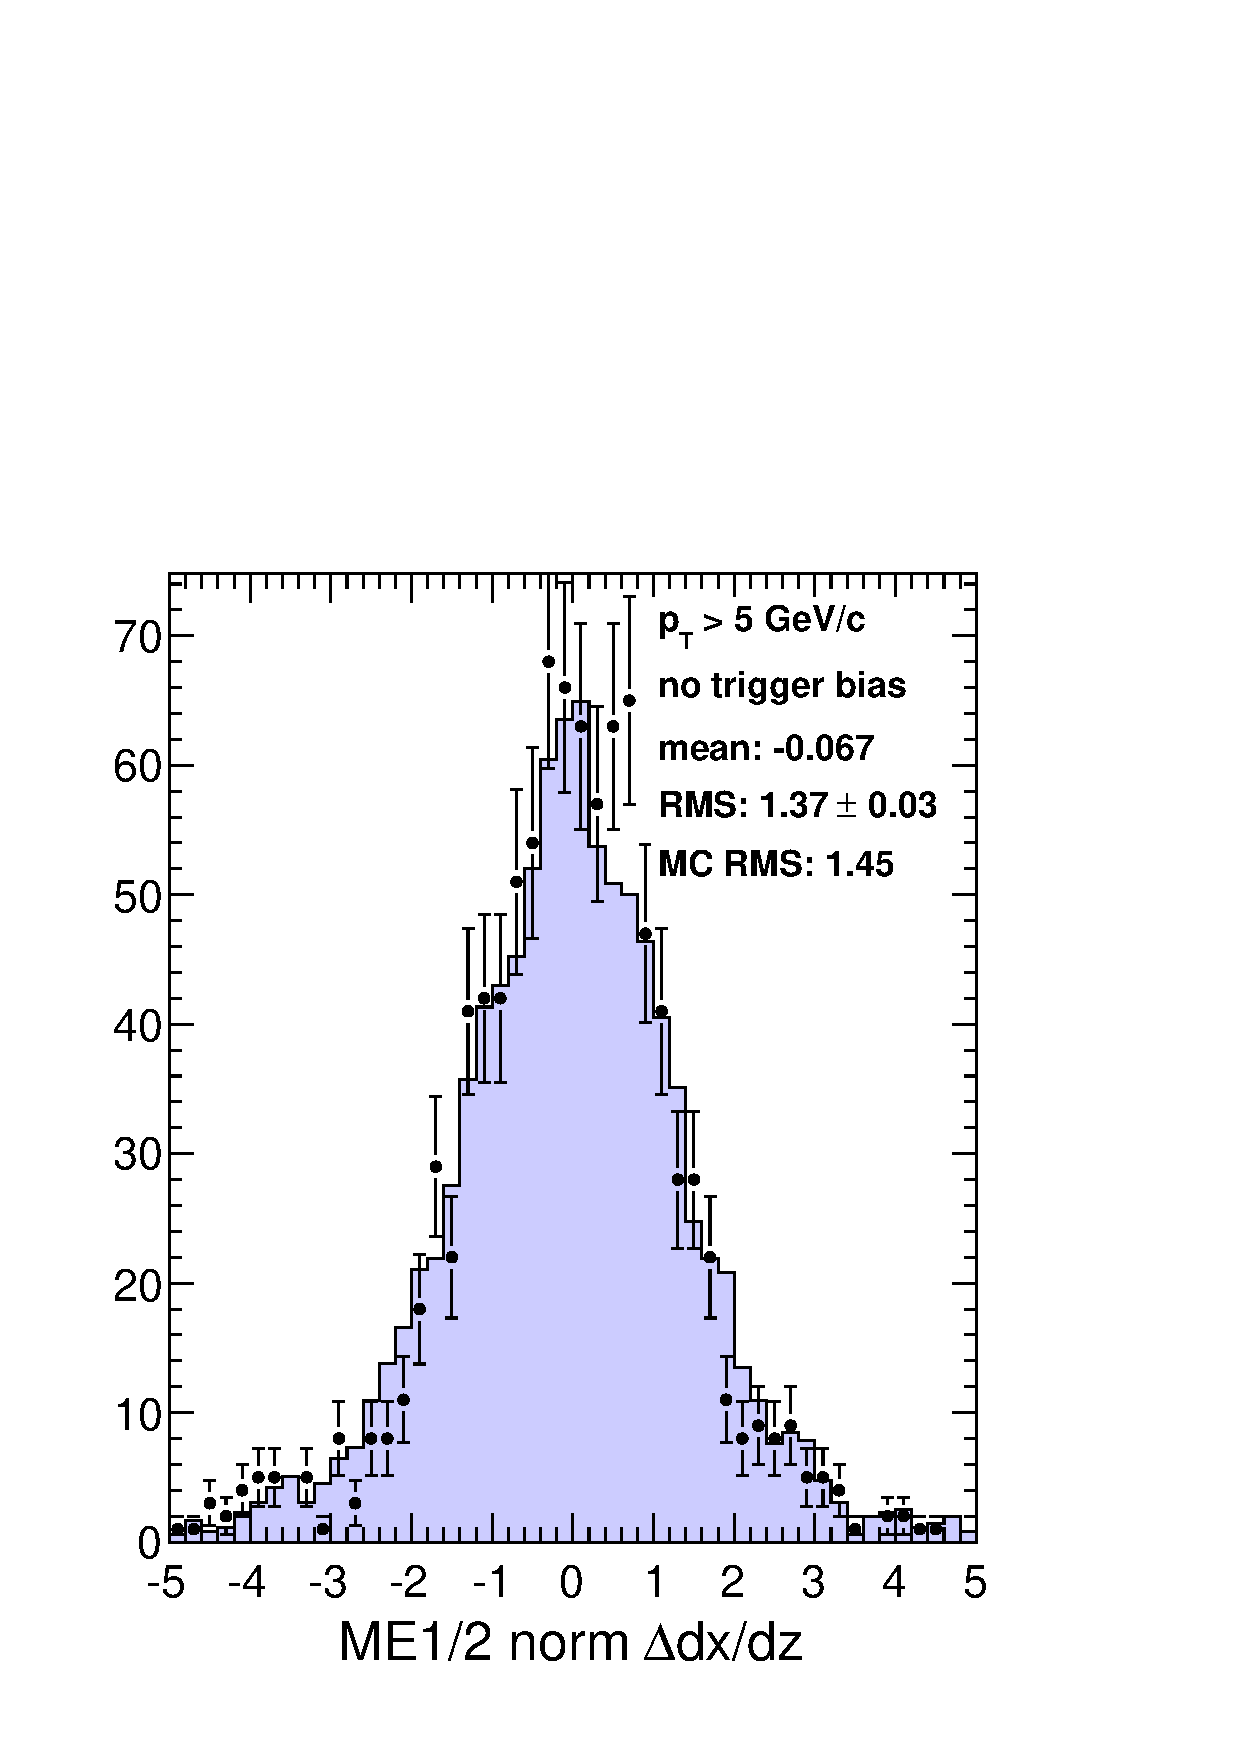
\includegraphics[width=\linewidth]{me12_dXdZnorm.pdf}
\end{columns}
\end{frame}

\begin{frame}
\frametitle{Summary plots}

\begin{itemize}
\item The same can be said for $dy/dz$ in the barrel
\item Discrepancy in MB0/2 and MB0/3: MC has large tails\ldots?
\end{itemize}
\begin{columns}
\column{0.8\linewidth}
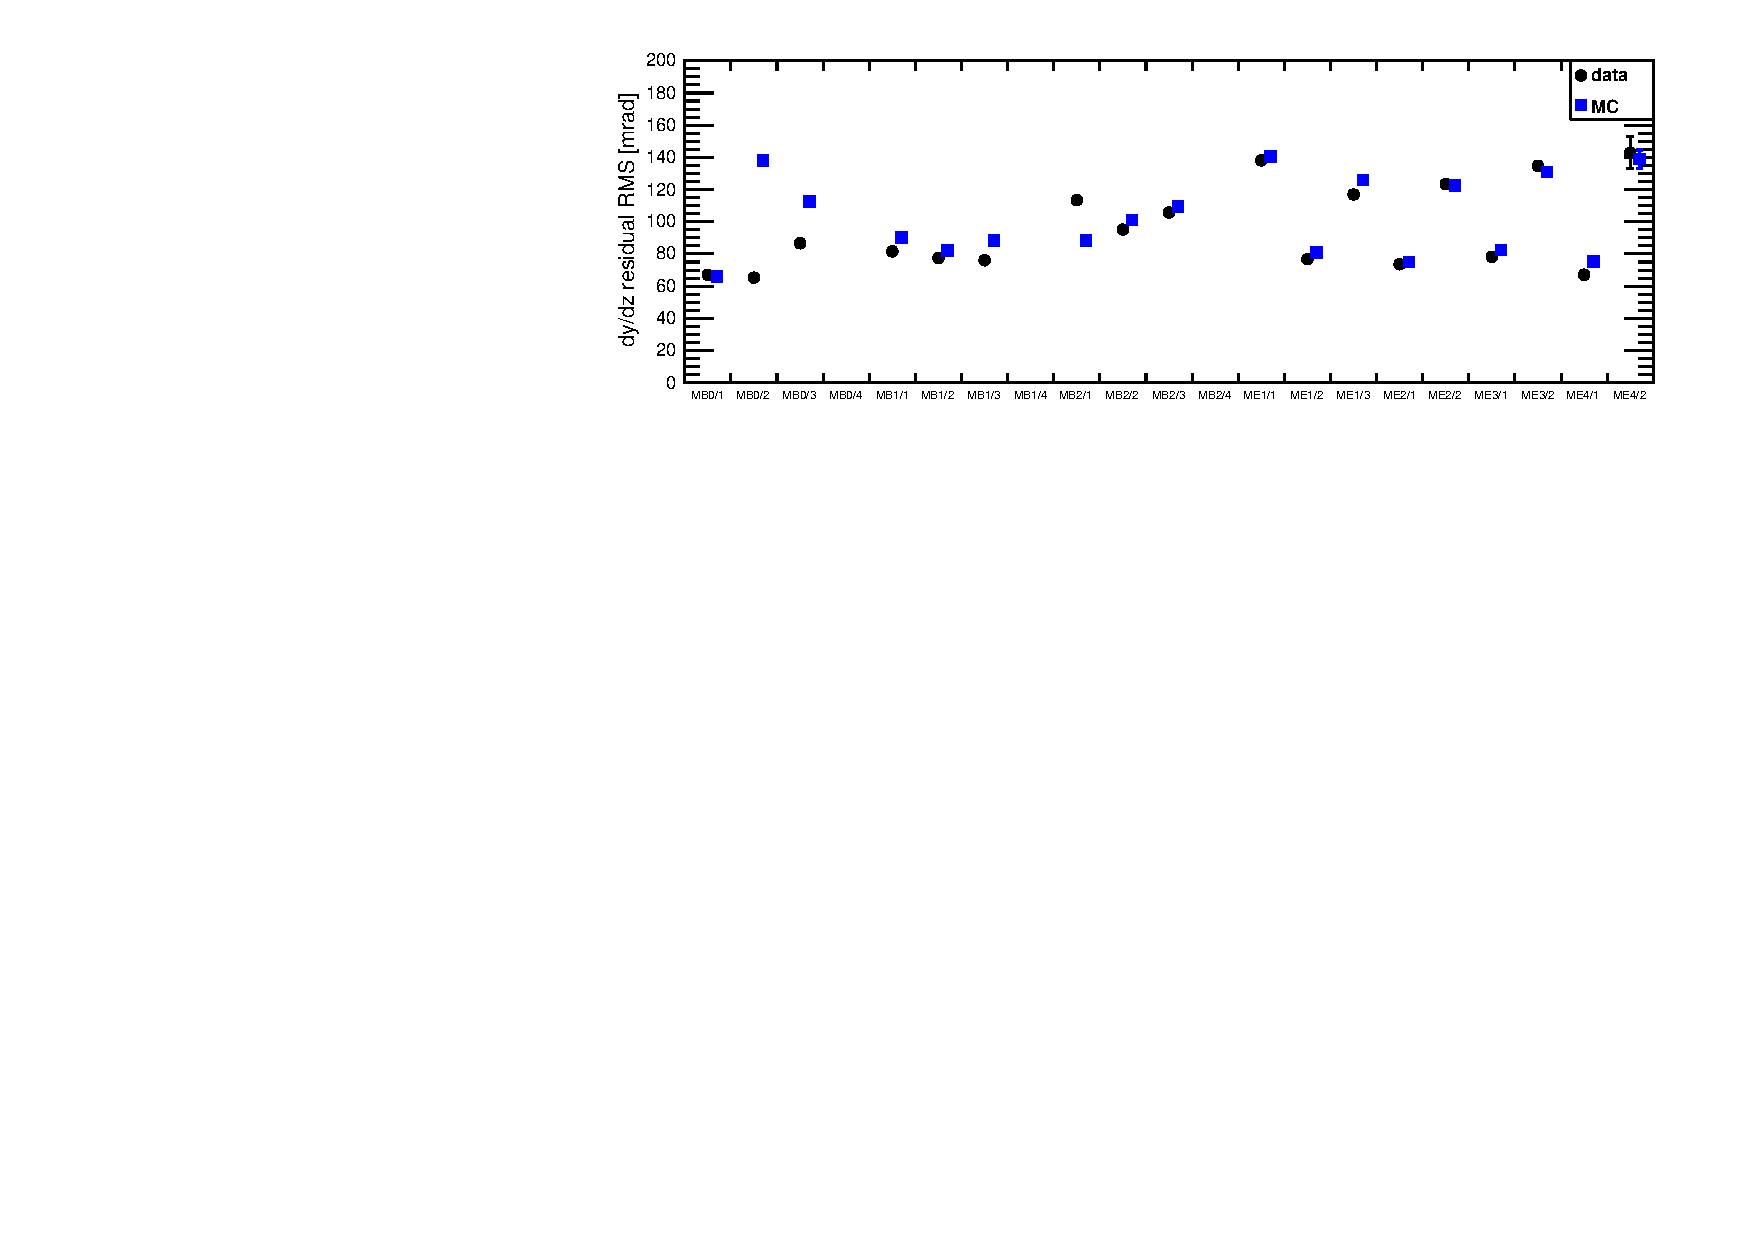
\includegraphics[width=\linewidth]{summarydYdZ.pdf}

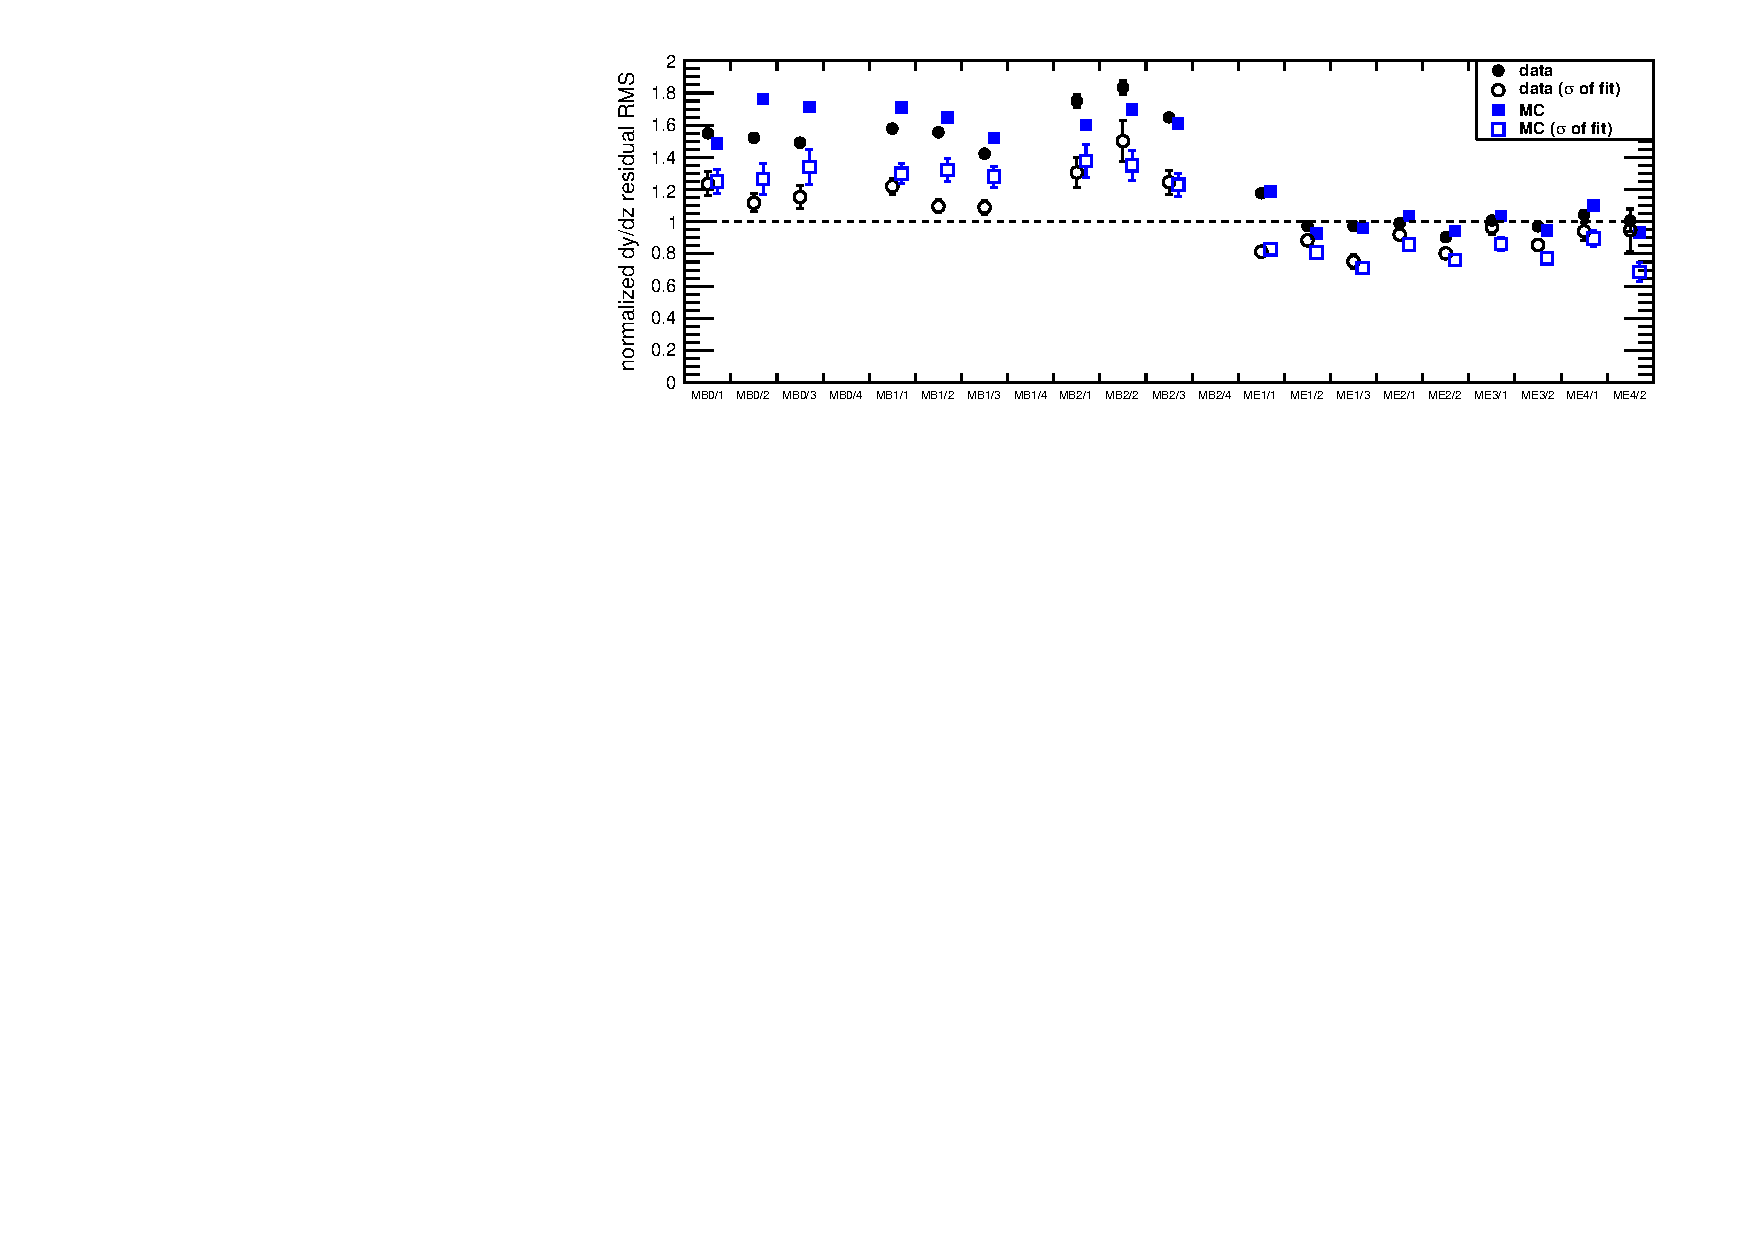
\includegraphics[width=\linewidth]{summarydYdZnorm.pdf}

\column{0.2\linewidth}

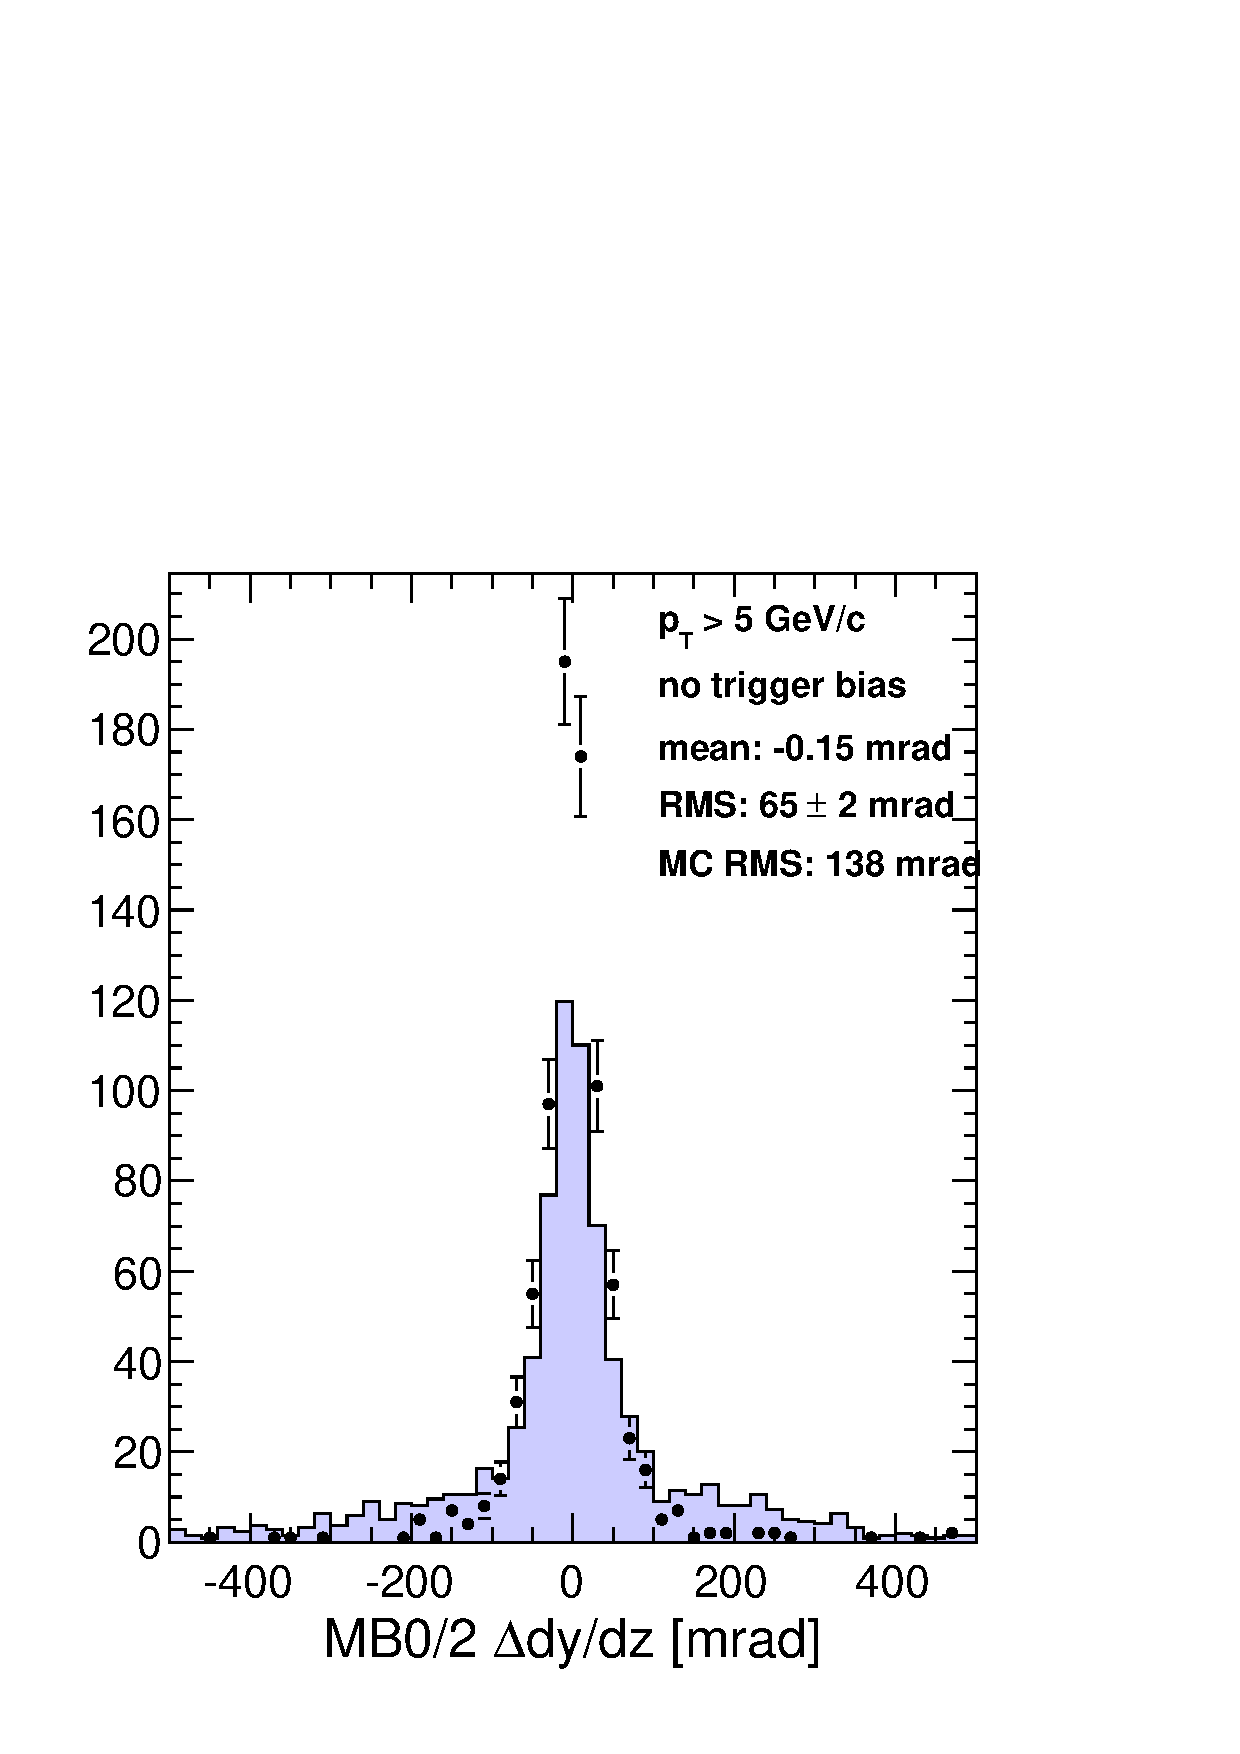
\includegraphics[width=\linewidth]{mb02_dYdZ.pdf}

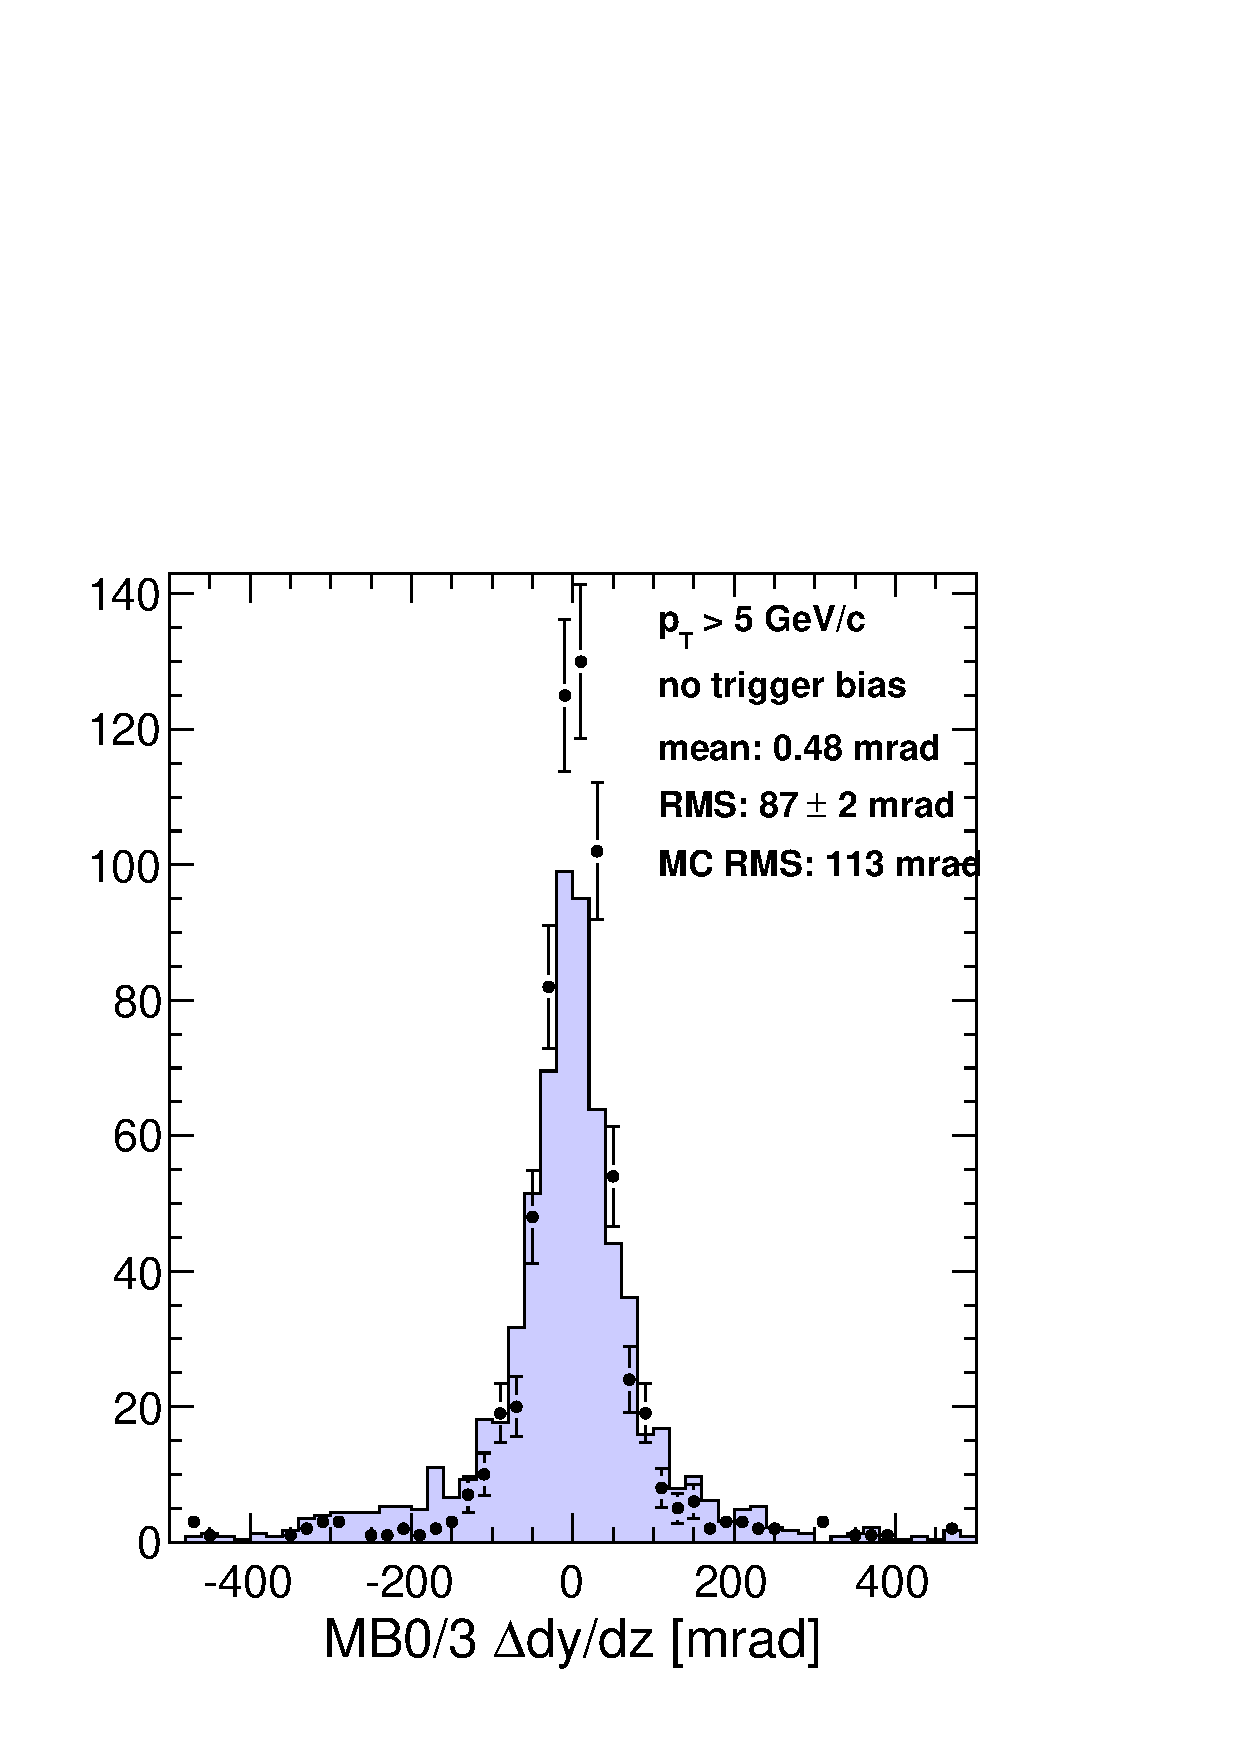
\includegraphics[width=\linewidth]{mb03_dYdZ.pdf}
\end{columns}
\end{frame}

\begin{frame}
\frametitle{Summary plots}

\begin{itemize}
\item Oddity in endcap: discrete peaks in $\Delta \frac{dy}{dz}$ residuals, reproduced by Monte Carlo and observed in standard RelVal plots (right)
\item Could be related to granularity of CSC wire-groups?
\item Note: we never use $\Delta y$ or $\Delta \frac{dy}{dz}$ in CSC alignment because of the granularity of wire-groups
\end{itemize}

\vfill
\begin{center}
\mbox{ } \hfill 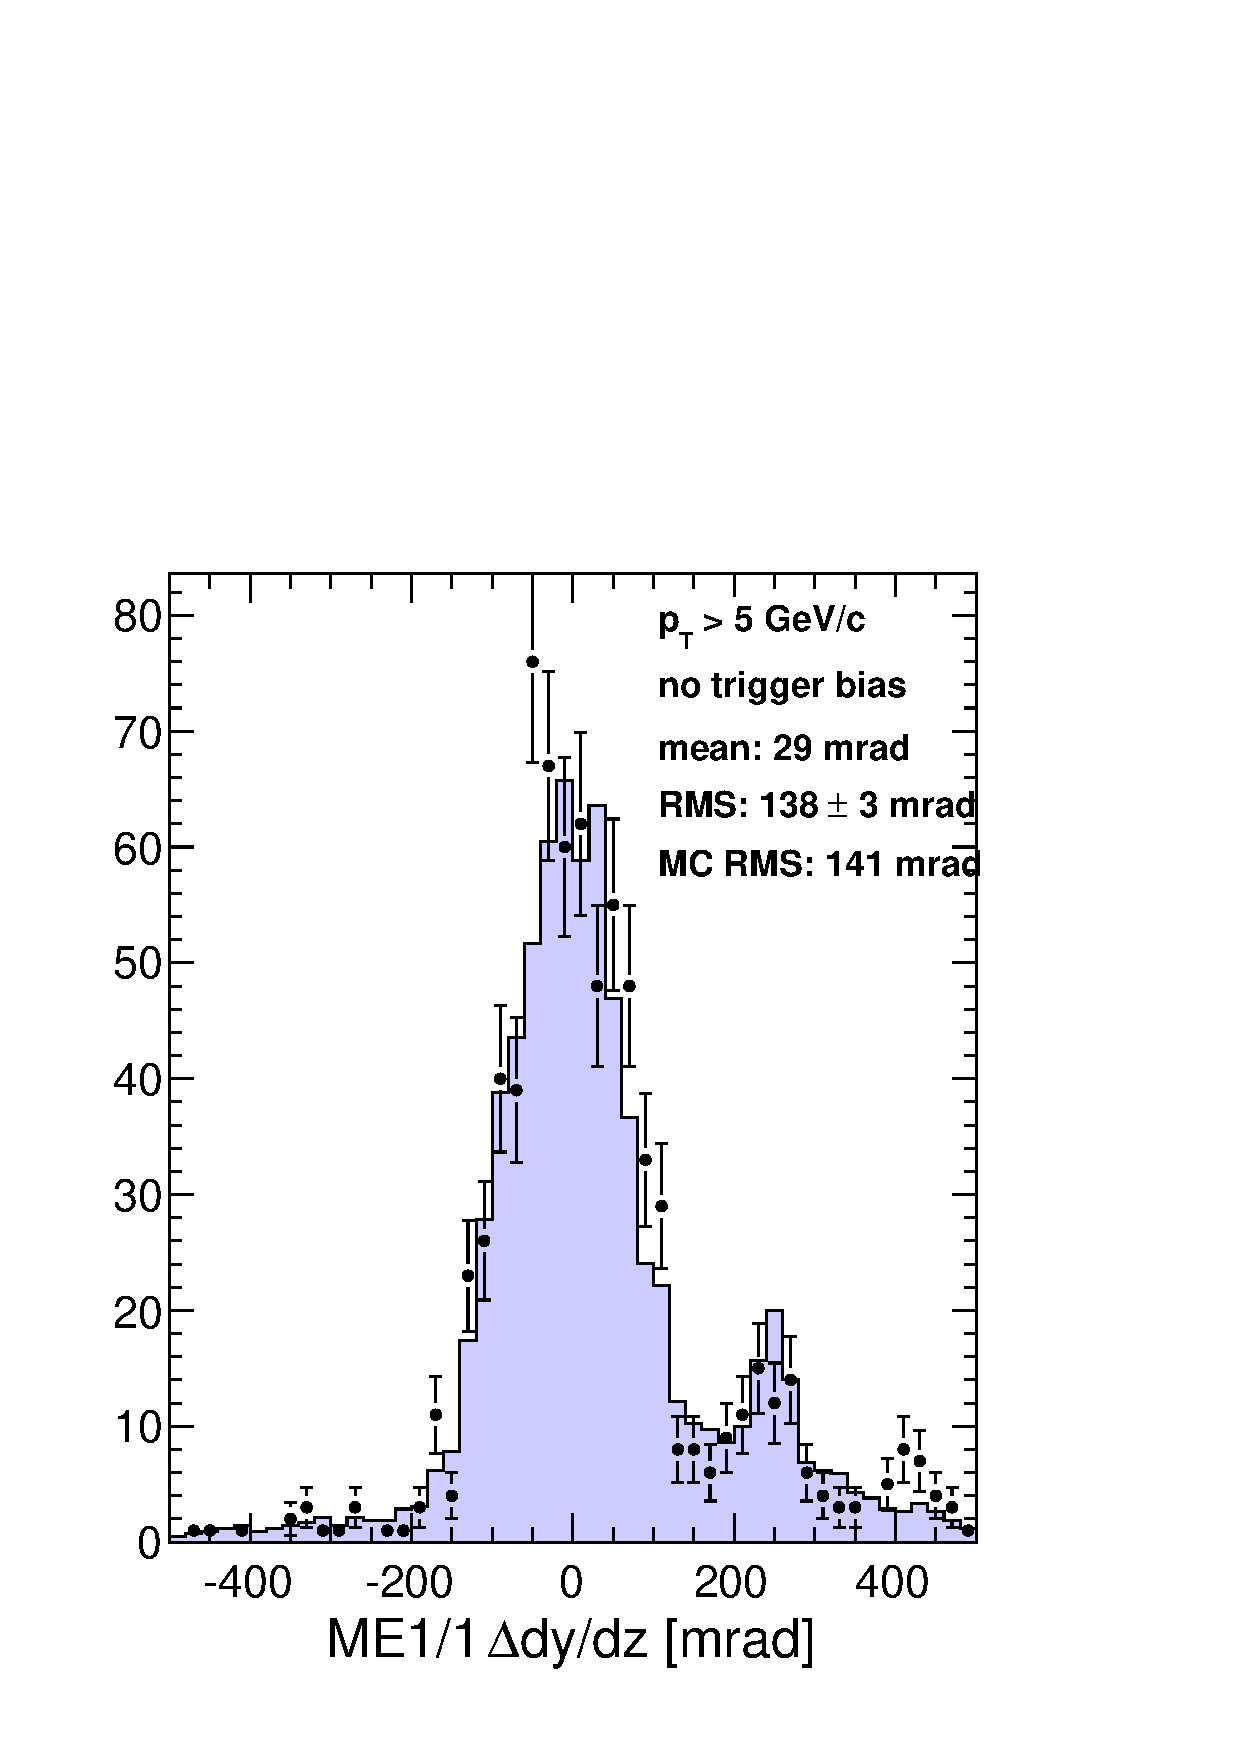
\includegraphics[height=3.2 cm]{me11_dYdZ.pdf} \hfill 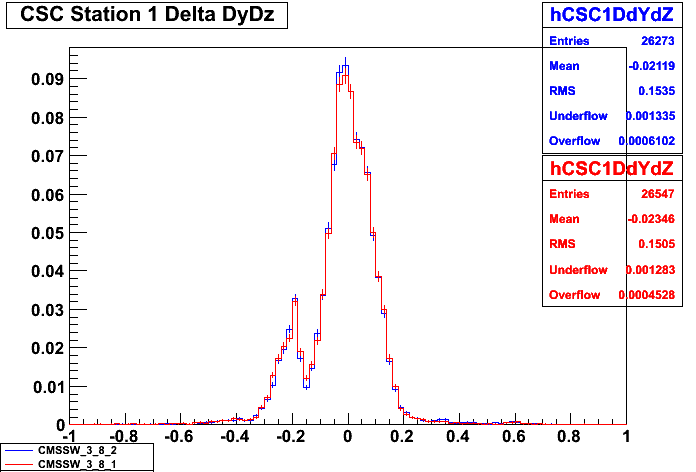
\includegraphics[height=3.2 cm]{me11_dydz_relvals.png} \hfill \mbox{ }
\end{center}

\vfill
\hspace{-0.83 cm} \textcolor{darkblue}{\Large Full set of plots}
\begin{itemize}
\item All of the individual residuals plots with data/MC overlays are in the backups
\end{itemize}
\end{frame}

\begin{frame}
\frametitle{Dependence on momentum}

\begin{columns}
\column{0.4\linewidth}
\begin{itemize}
\item Plot $\phi = x/R$ residuals from MB3 and ME2

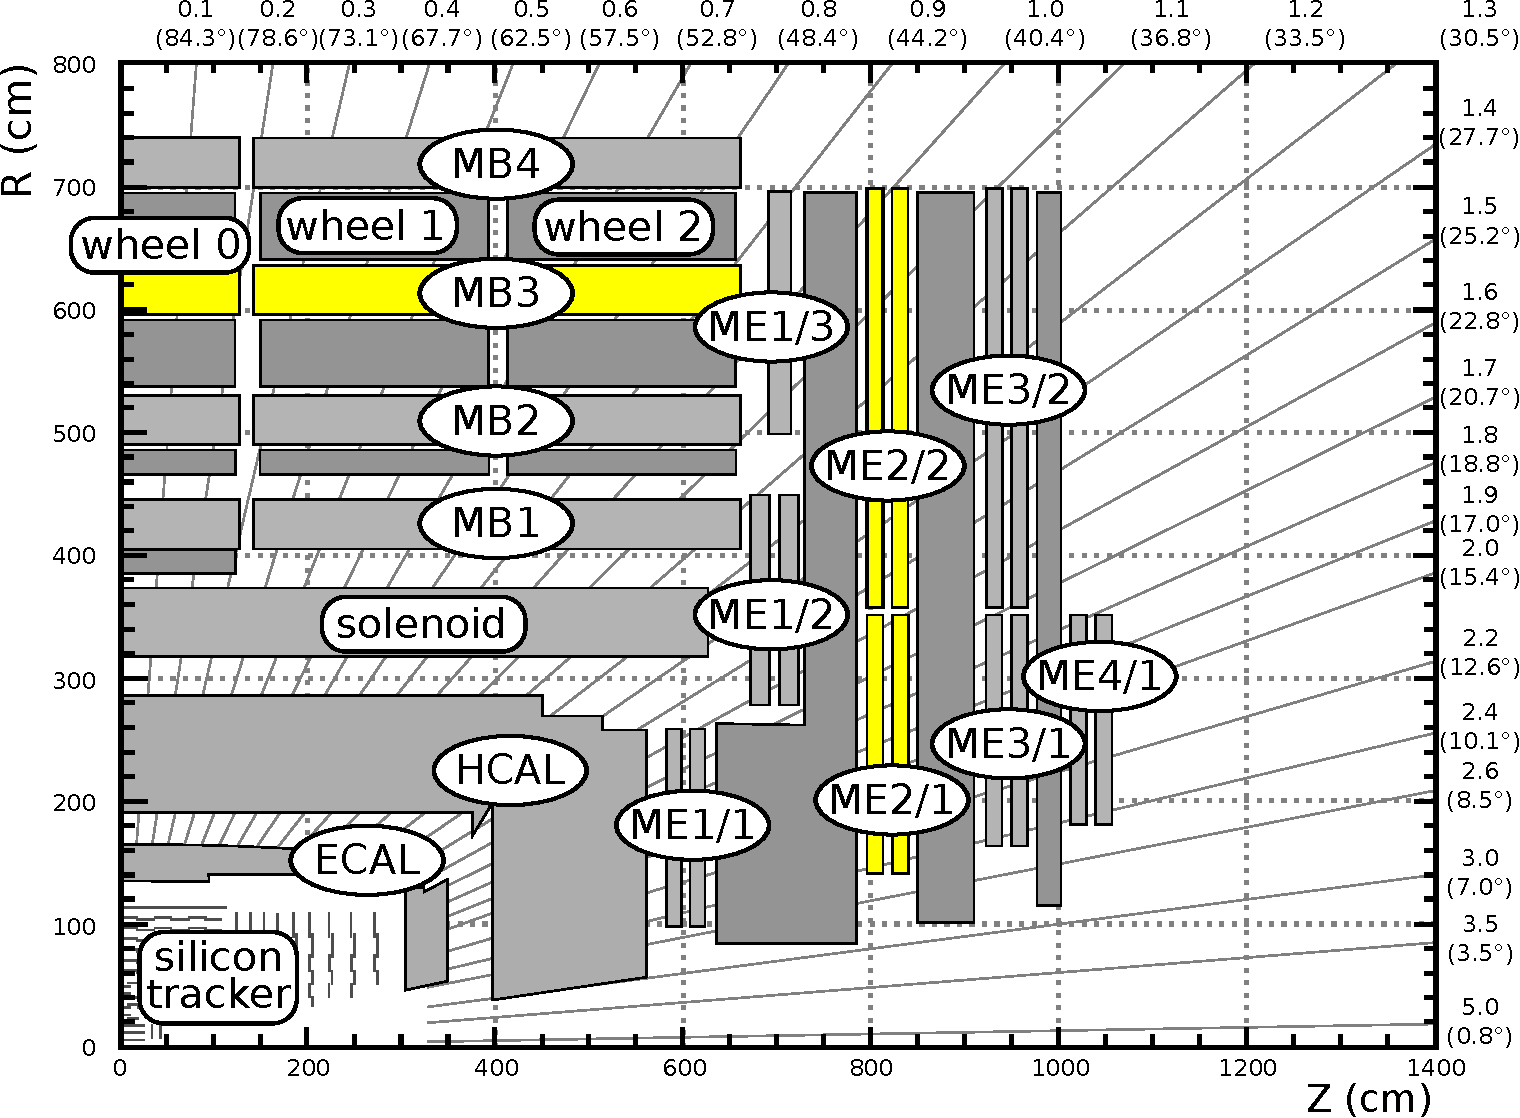
\includegraphics[width=\linewidth]{muon_system_labeled_mb3-me2.pdf}

(one representative residual per track)

\item Width of residuals distribution scales roughly as $1/|p|$, cut at $1/p_T < 0.2$~$c$/GeV

\item Any biases in the mean are much smaller than the width of
  \mbox{the distribution\hspace{-1 cm}}
\end{itemize}

\column{0.6\linewidth}
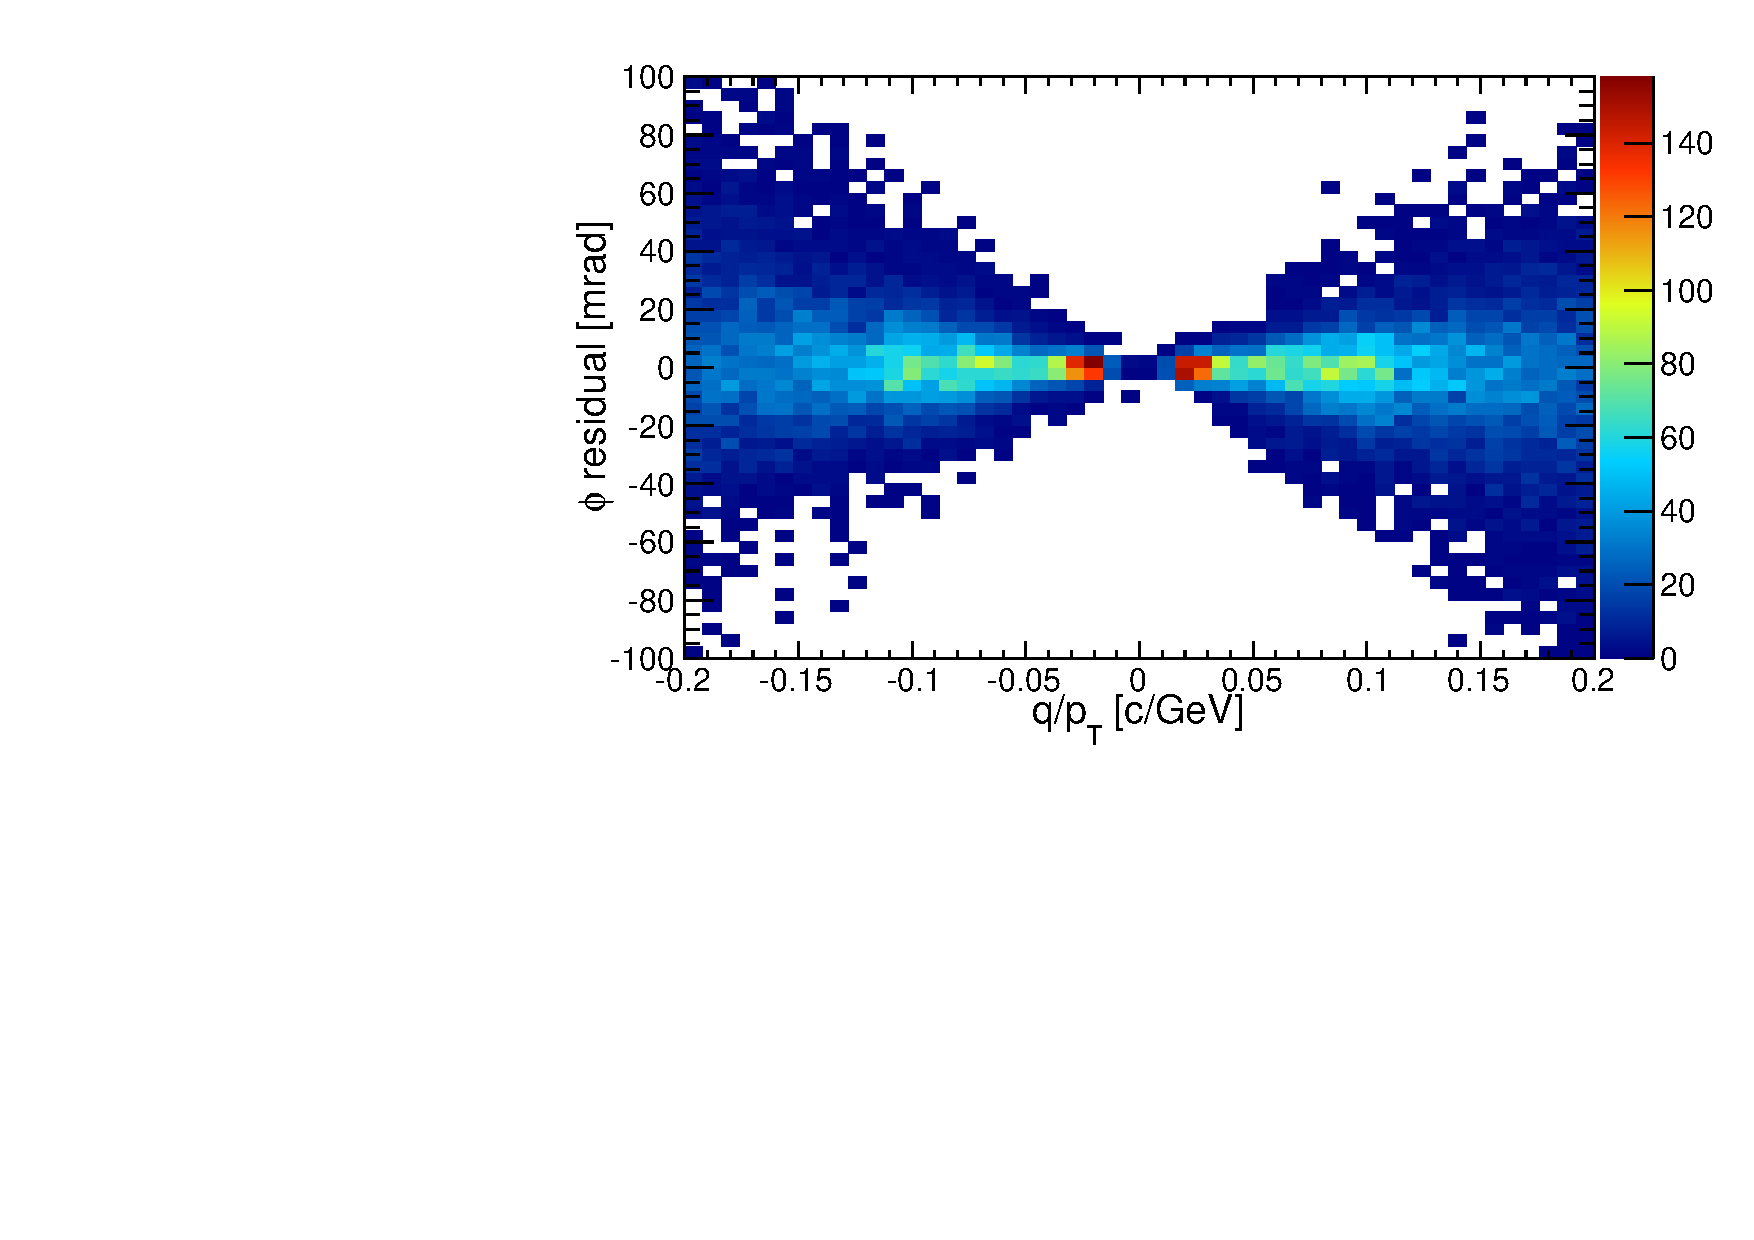
\includegraphics[width=\linewidth]{simple2d_qoverpt.pdf}

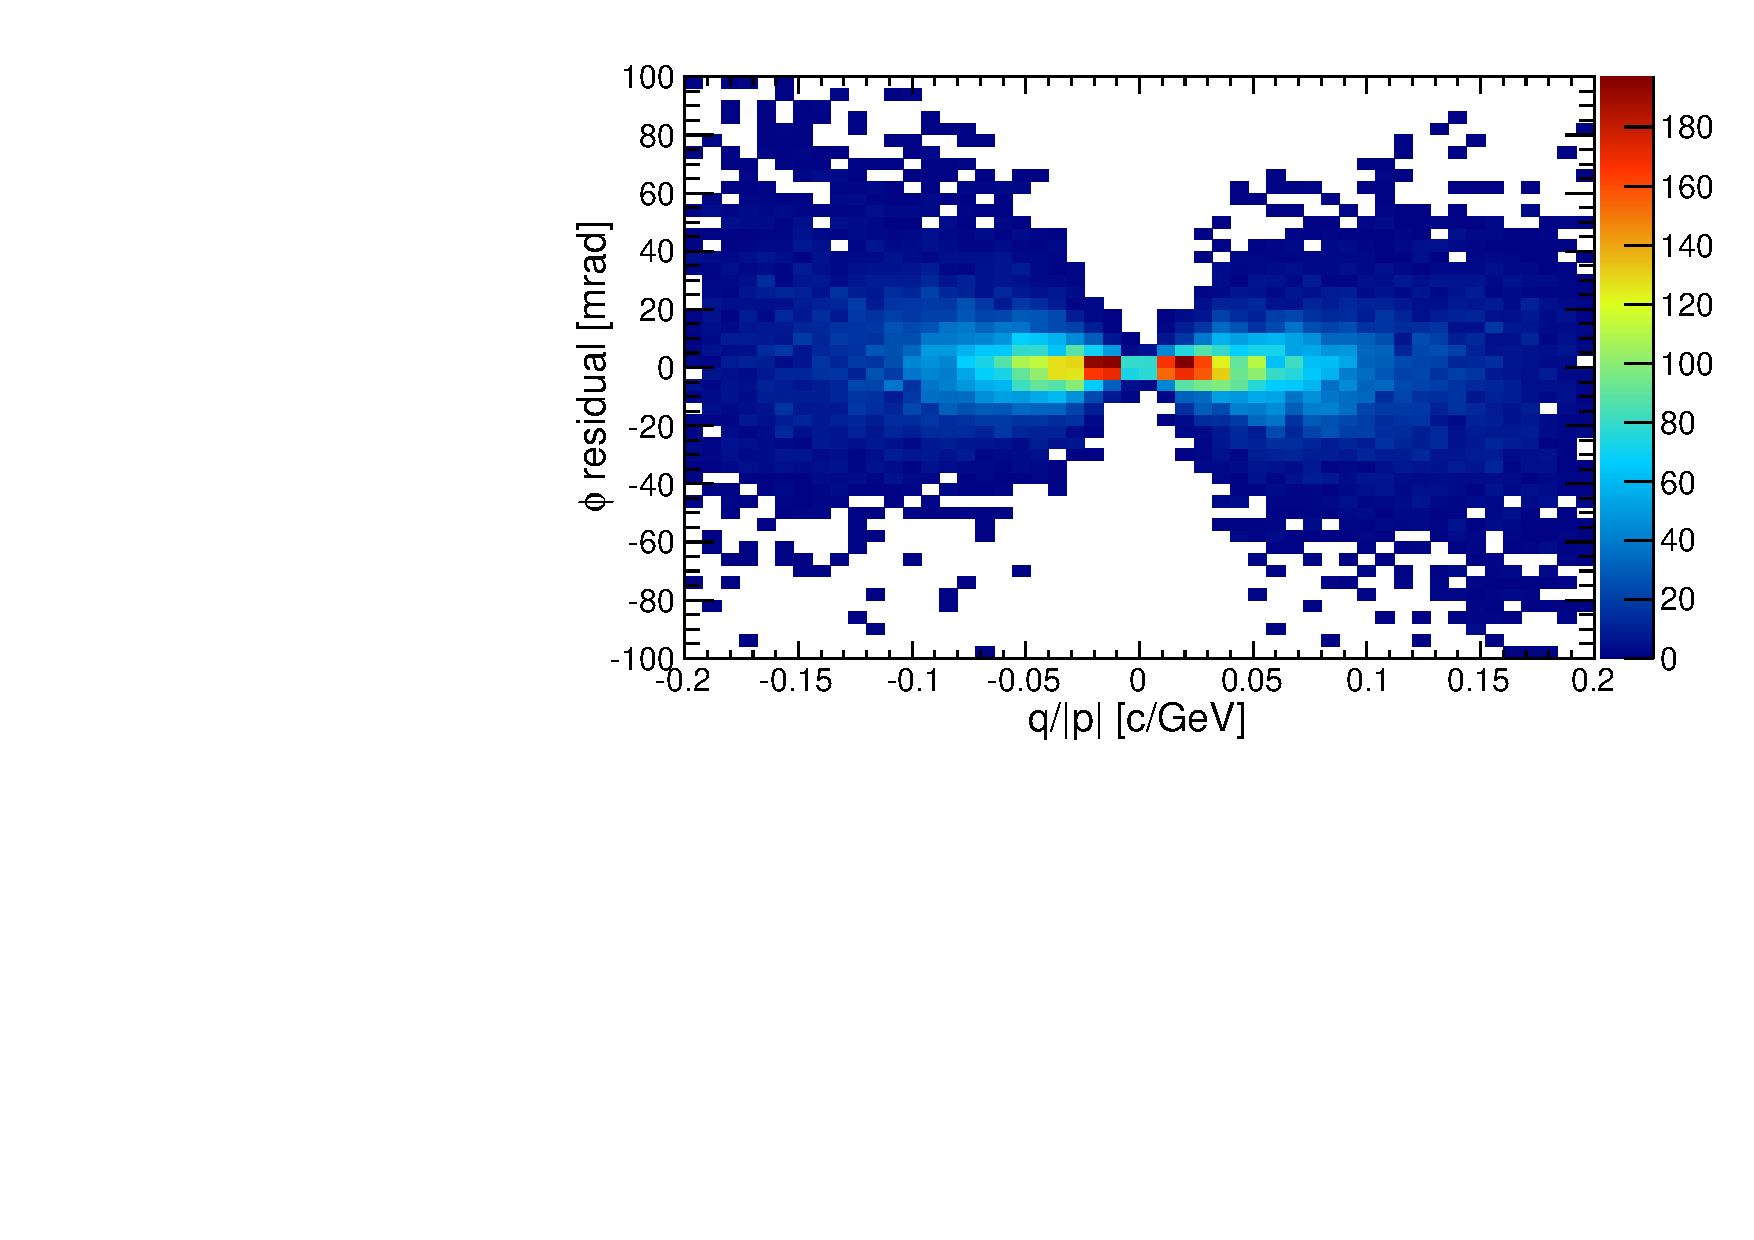
\includegraphics[width=\linewidth]{simple2d_qoverpmag.pdf}
\end{columns}
\end{frame}

\begin{frame}
\frametitle{Dependence on momentum}

\vspace{-1.8 cm}
\begin{itemize}
\item To quantify bias in the Gaussian part of the residuals peak (not
  the tails), fit distributions in momentum bins to
\[ p(x) = \left\{ \begin{array}{c c}
A \exp\left(-(x - x_0)^2/(2\sigma^2)\right) & |x - x_0| < m \\
B/|x|^{p_1} & (x - x_0) > m_1 \\
C/|x|^{p_2} & -(x - x_0) < -m_2 \\
\end{array} \right. \]

where $A$, $B$, $C$, $m_1$, and $m_2$ are chosen to make the function
continuous and differentiable (like alignment fit)
\end{itemize}

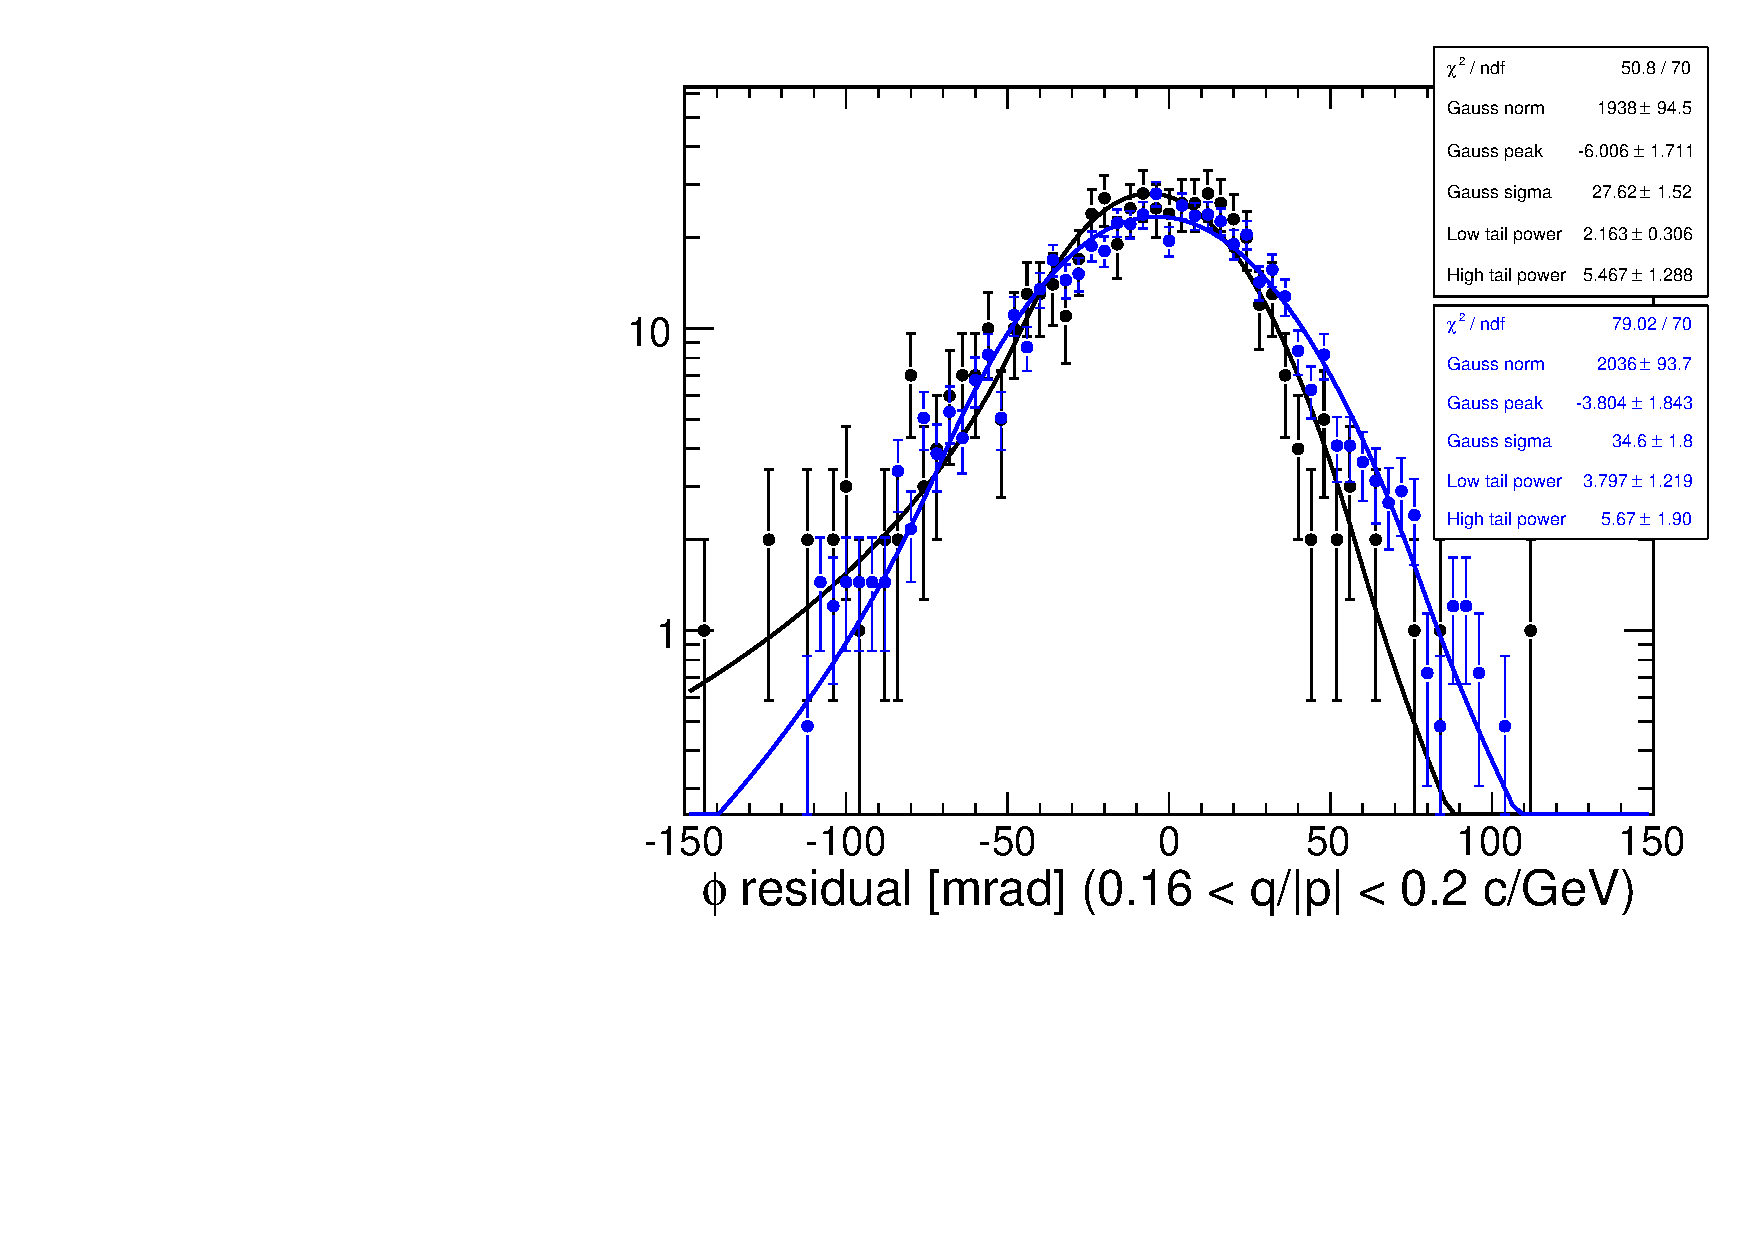
\includegraphics[width=0.49\linewidth]{example_lowmomentum.pdf}
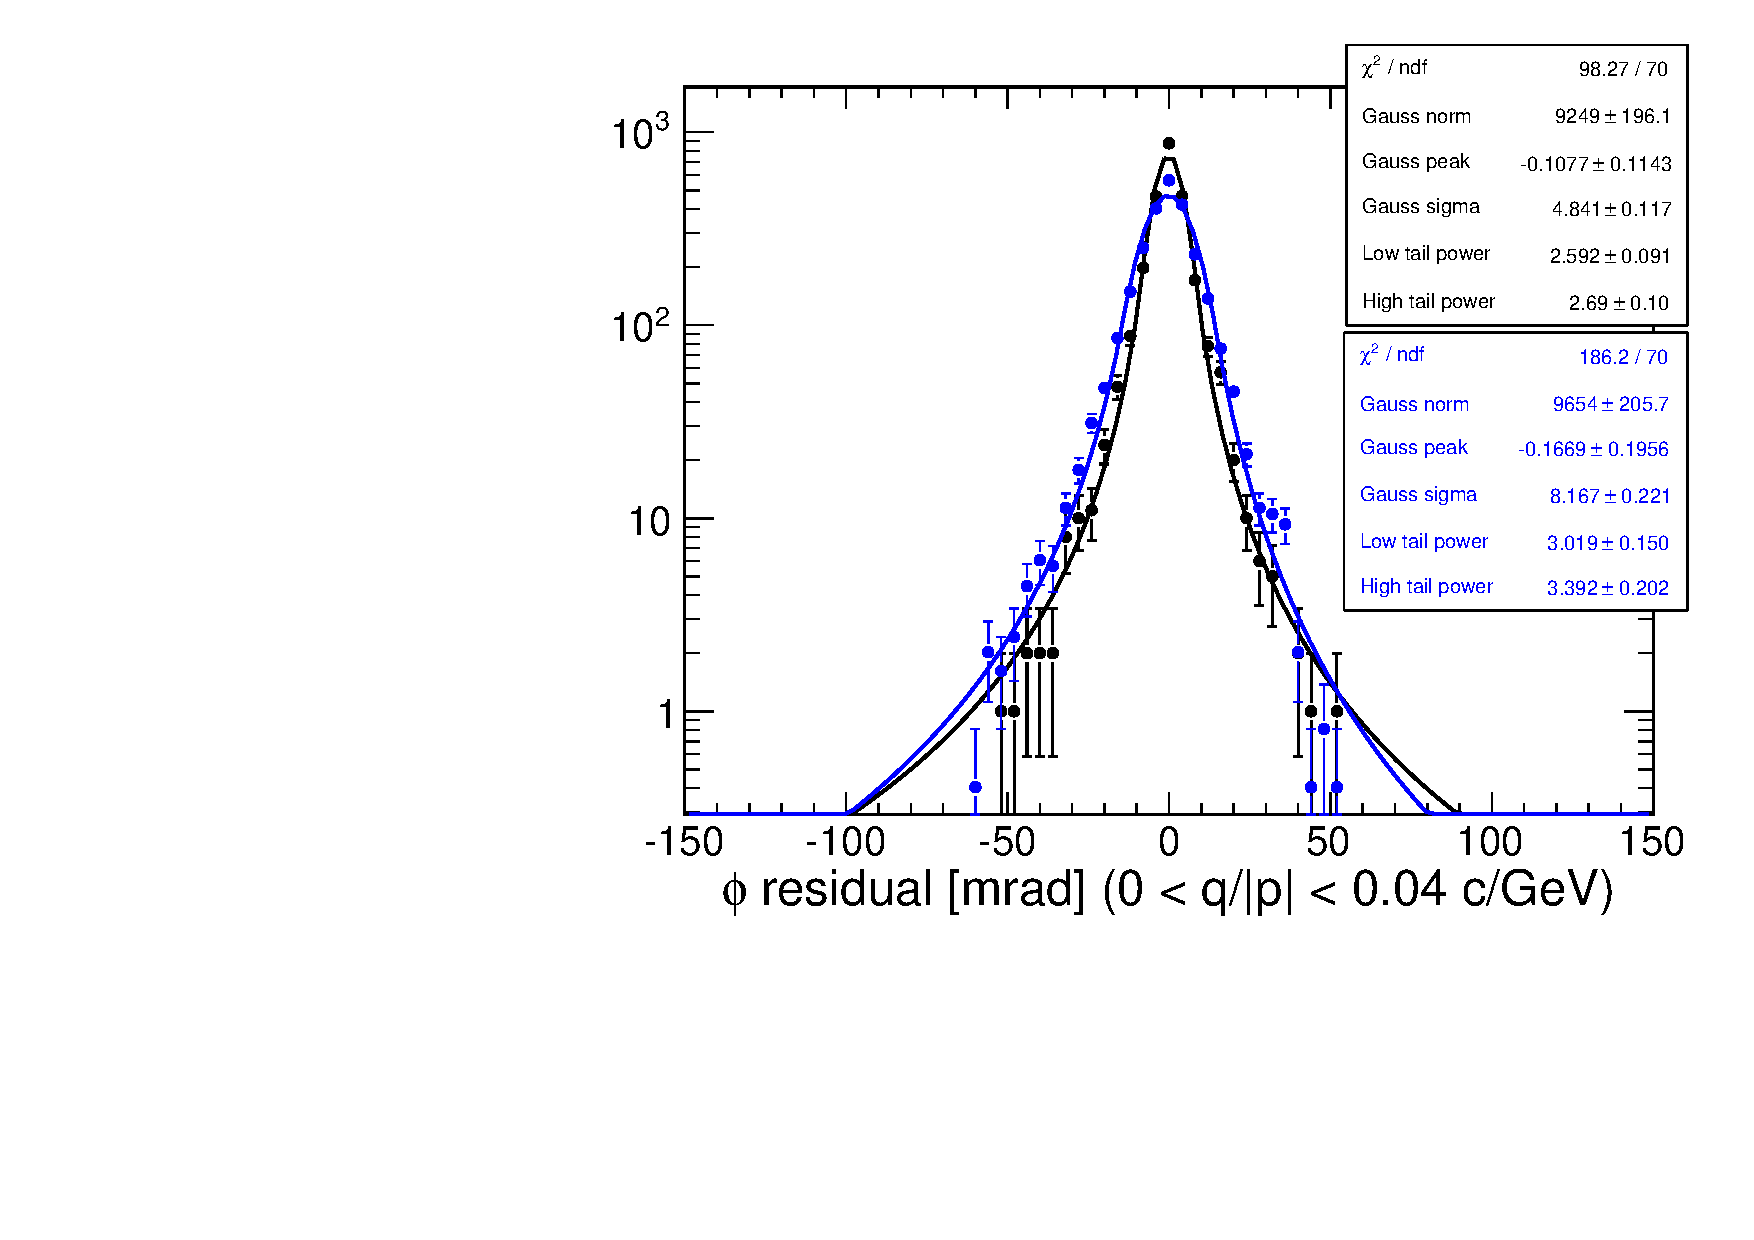
\includegraphics[width=0.49\linewidth]{example_highmomentum.pdf}

\vspace{-3.6 cm}
\hspace{6.3 cm}\textcolor{black}{data: black}

\hspace{6.3 cm}\textcolor{blue}{MC: blue}
\end{frame}

\begin{frame}
\frametitle{Dependence on momentum}
\begin{itemize}
\item There is a trend in residuals vs.\ inverse momentum that is
  partly in the tails, partly in the Gaussian peak of the distribution
\item \textcolor{black}{Black: data}, \textcolor{blue}{blue: Monte Carlo}

\begin{columns}
\column{0.5\linewidth}
\begin{center}
Mean of each bin vs.\ $q/|p|$
\end{center}
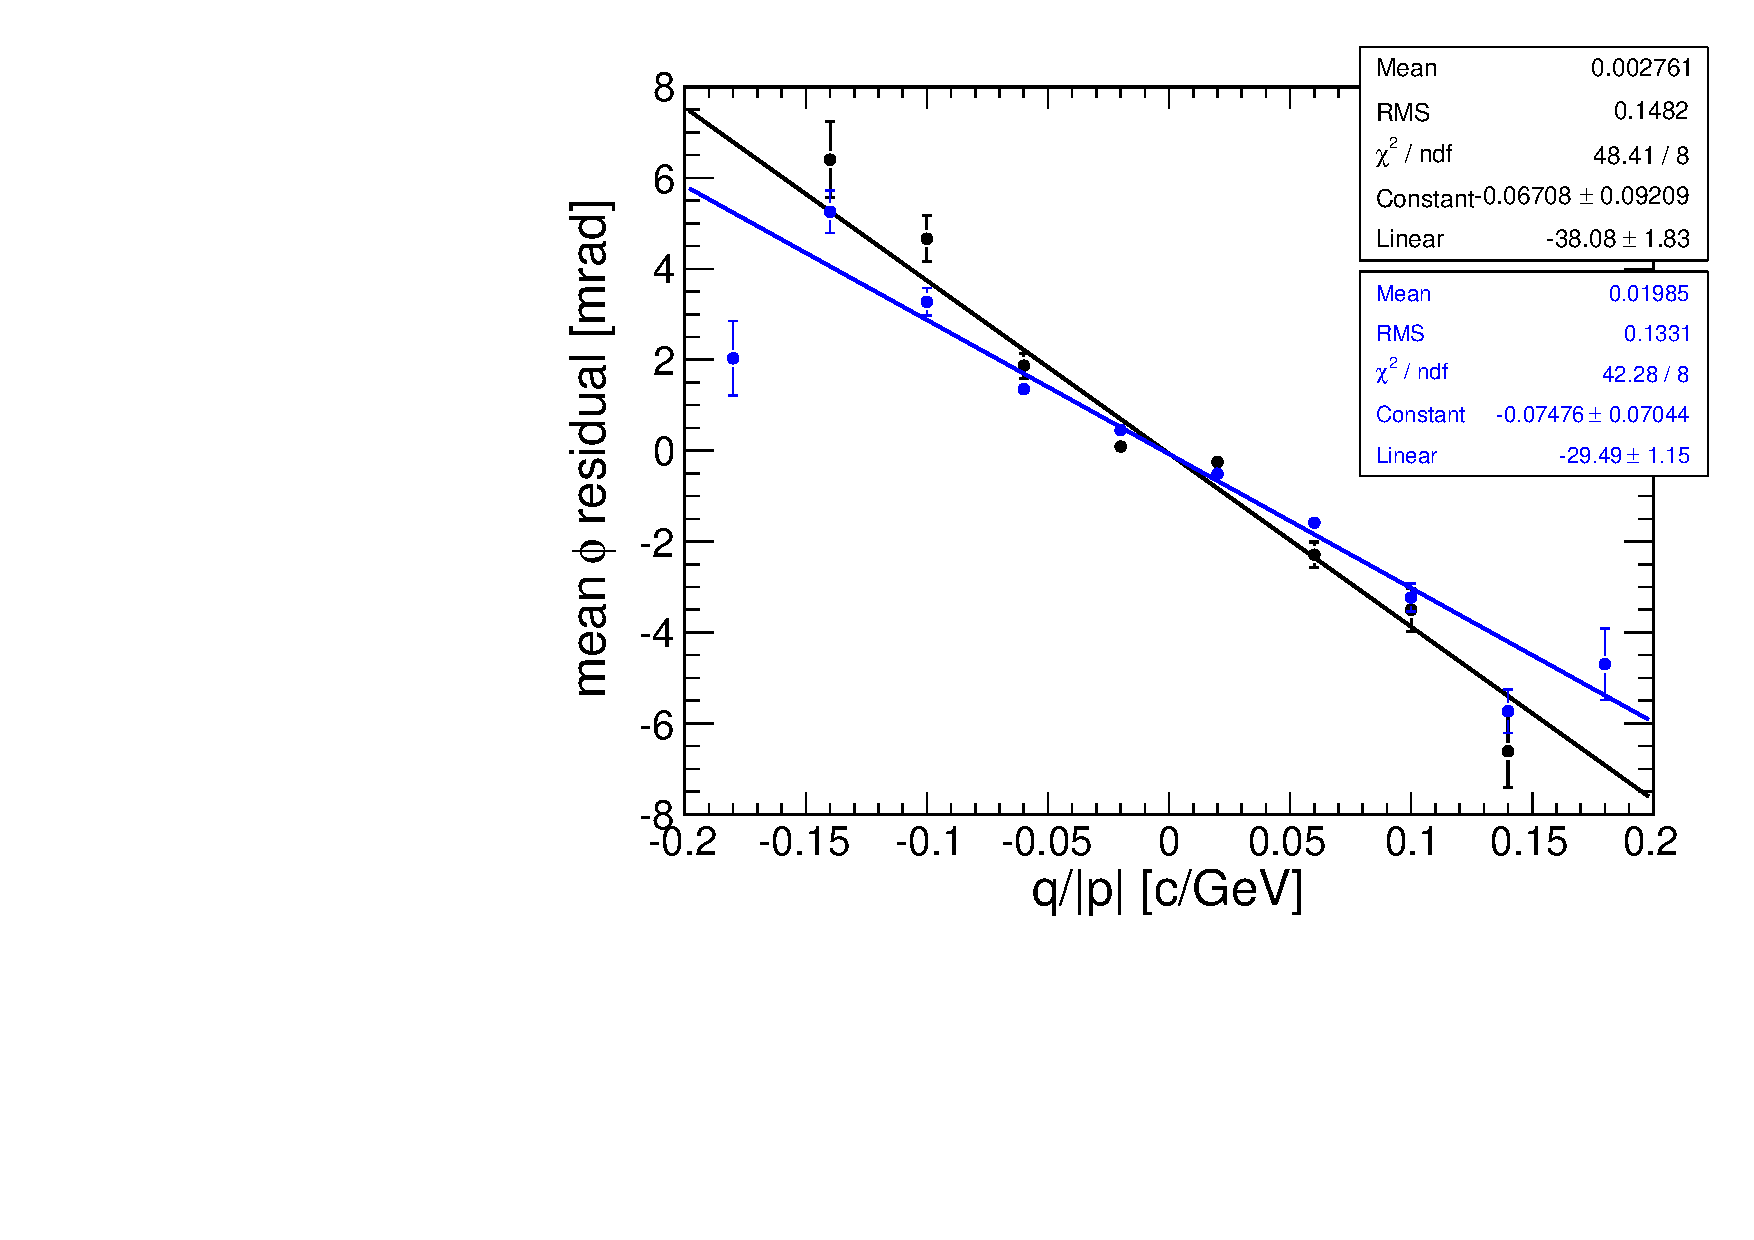
\includegraphics[width=\linewidth]{nocuts_means.pdf}

\column{0.5\linewidth}
\begin{center}
Fitted peak of each bin vs.\ $q/|p|$
\end{center}
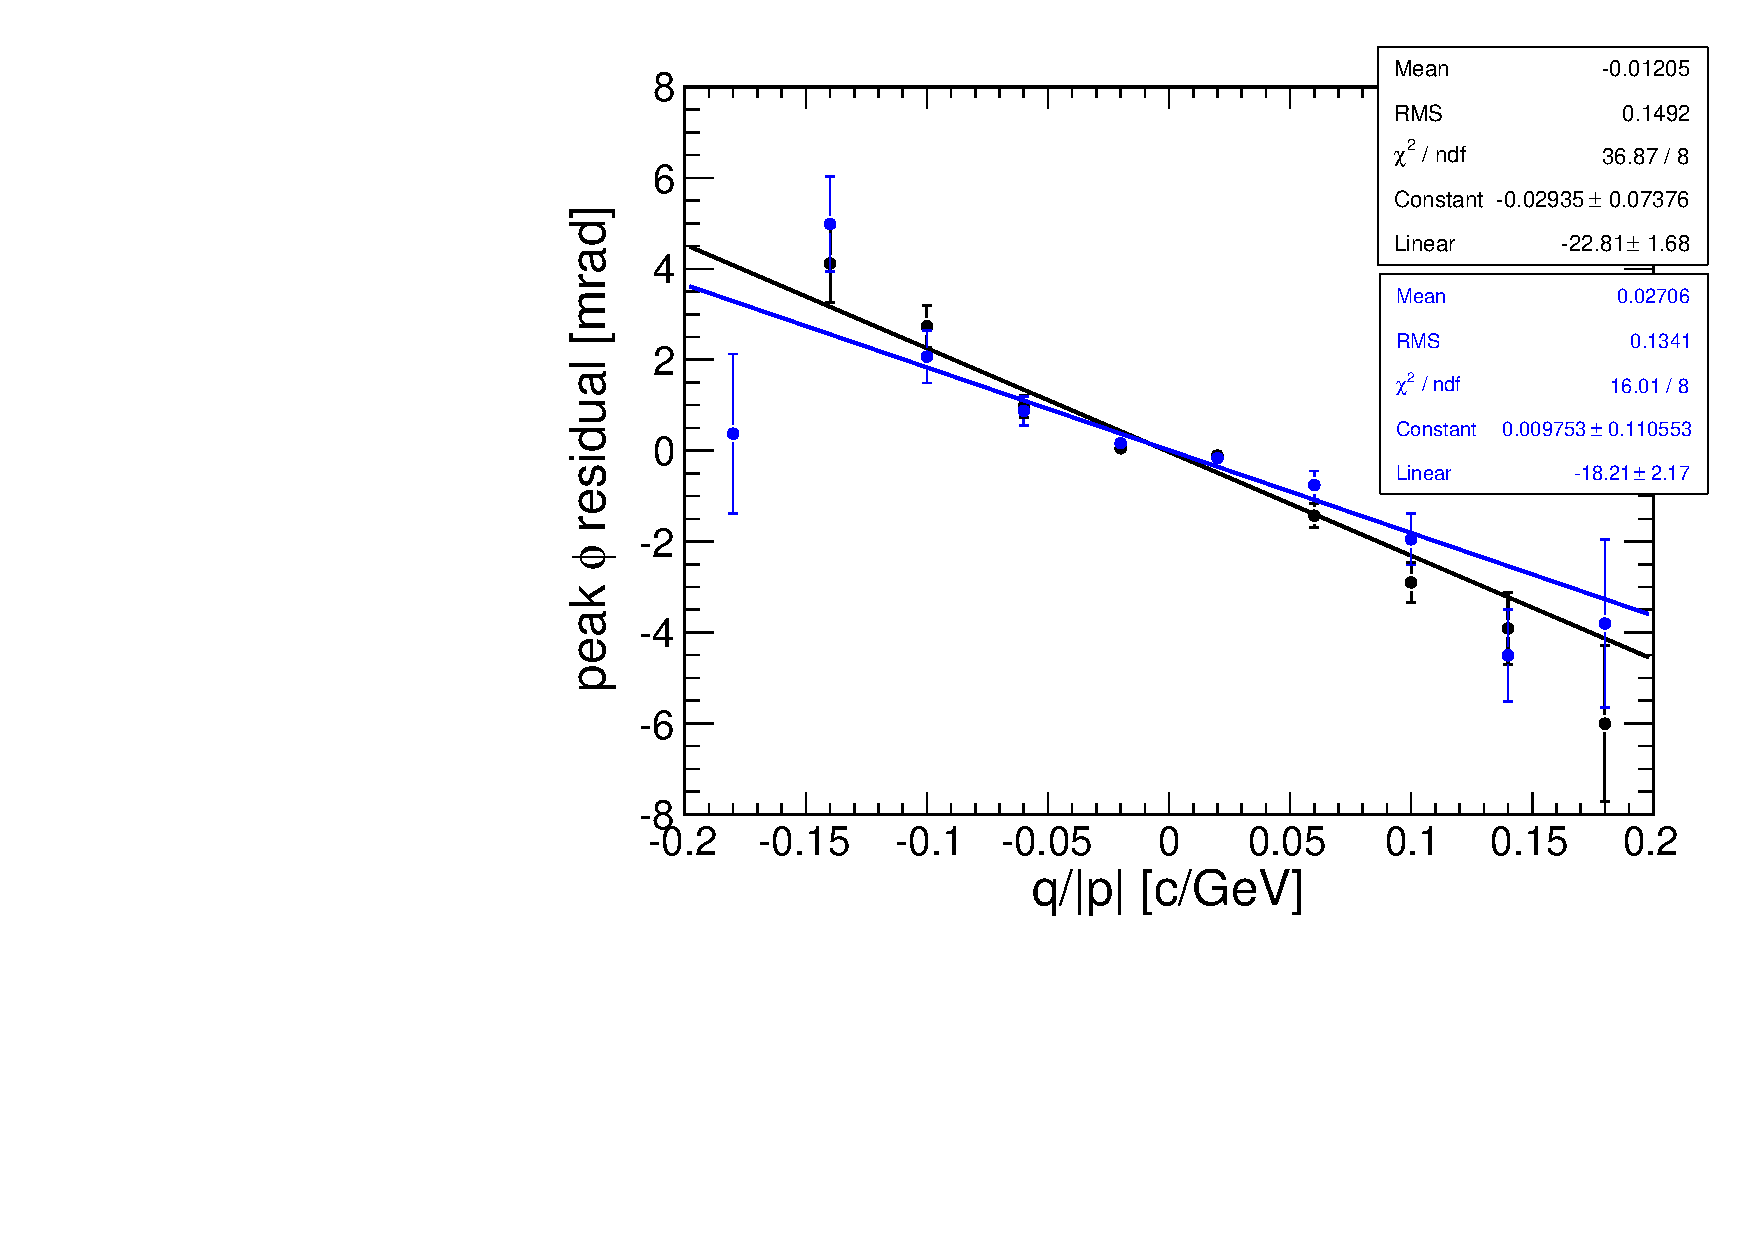
\includegraphics[width=\linewidth]{nocuts_gausspeak.pdf}
\end{columns}
\end{itemize}
\end{frame}

\begin{frame}
\frametitle{Dependence on momentum}
\begin{itemize}
\item However, decays-in-flight can bias the residuals distribution in exactly this way
\item In Monte Carlo, we can ask that none of the muons come from a
  $\pi^\pm$ or $K^\pm$ decay
\item \textcolor{blue}{Blue: the MC you saw on the previous page},
  \textcolor{red}{red: same with no decays-in-flight}

\begin{center}
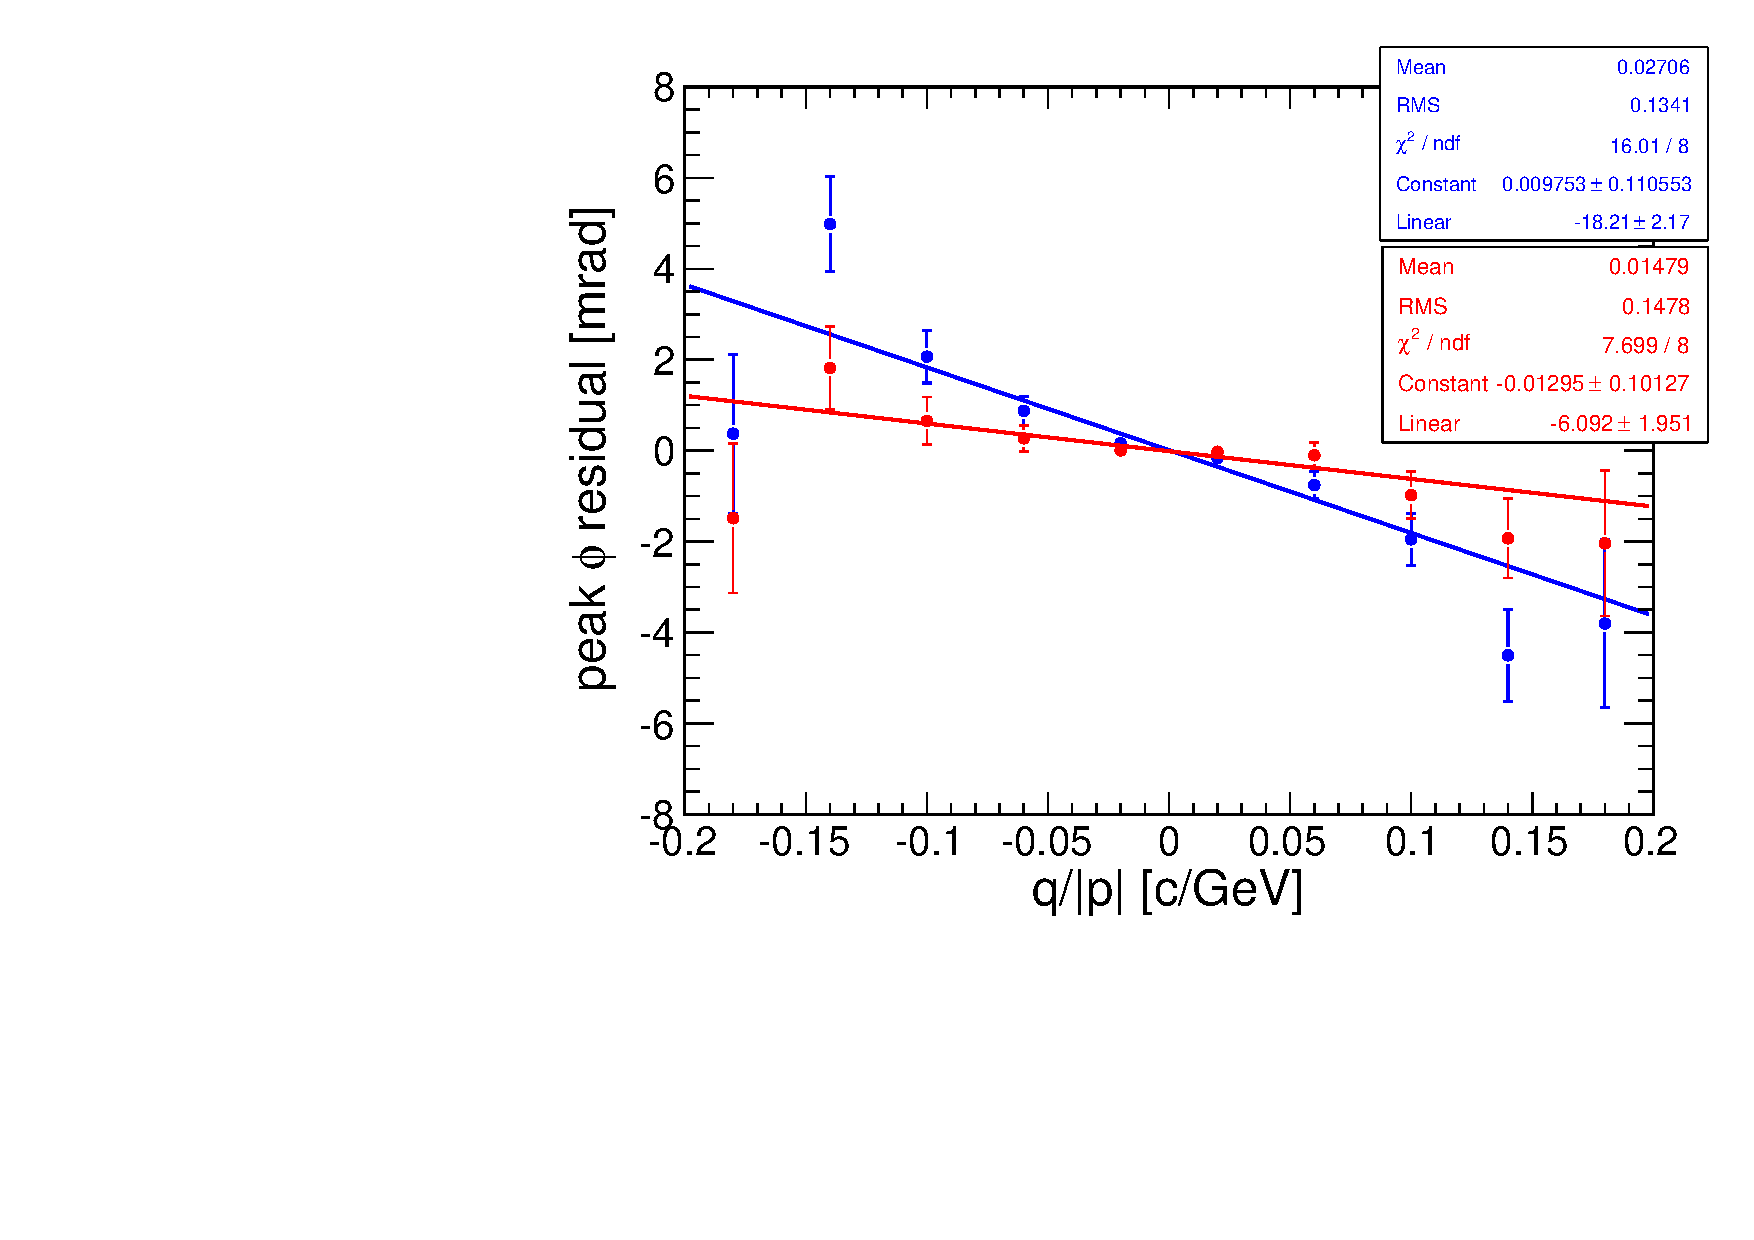
\includegraphics[width=0.5\linewidth]{nocuts_decayinflight.pdf}
\end{center}
\end{itemize}
\end{frame}

\begin{frame}
\frametitle{Dependence on momentum}
\begin{columns}
\column{0.8\linewidth}
\begin{itemize}
\item To suppress decays-in-flight in data, we require muons to come
  from a $J/\psi$ ($\pm 0.2$~GeV/$c^2$; right)
\item We are left with a bias in data but not Monte
  Carlo: about 15\% of the width of the 5~GeV/$c$ distribution
\item Do we see the same in GlobalMuon cosmic rays?
\item \textcolor{black}{Black: data}, \textcolor{blue}{blue: Monte Carlo}
\end{itemize}

\column{0.2\linewidth}
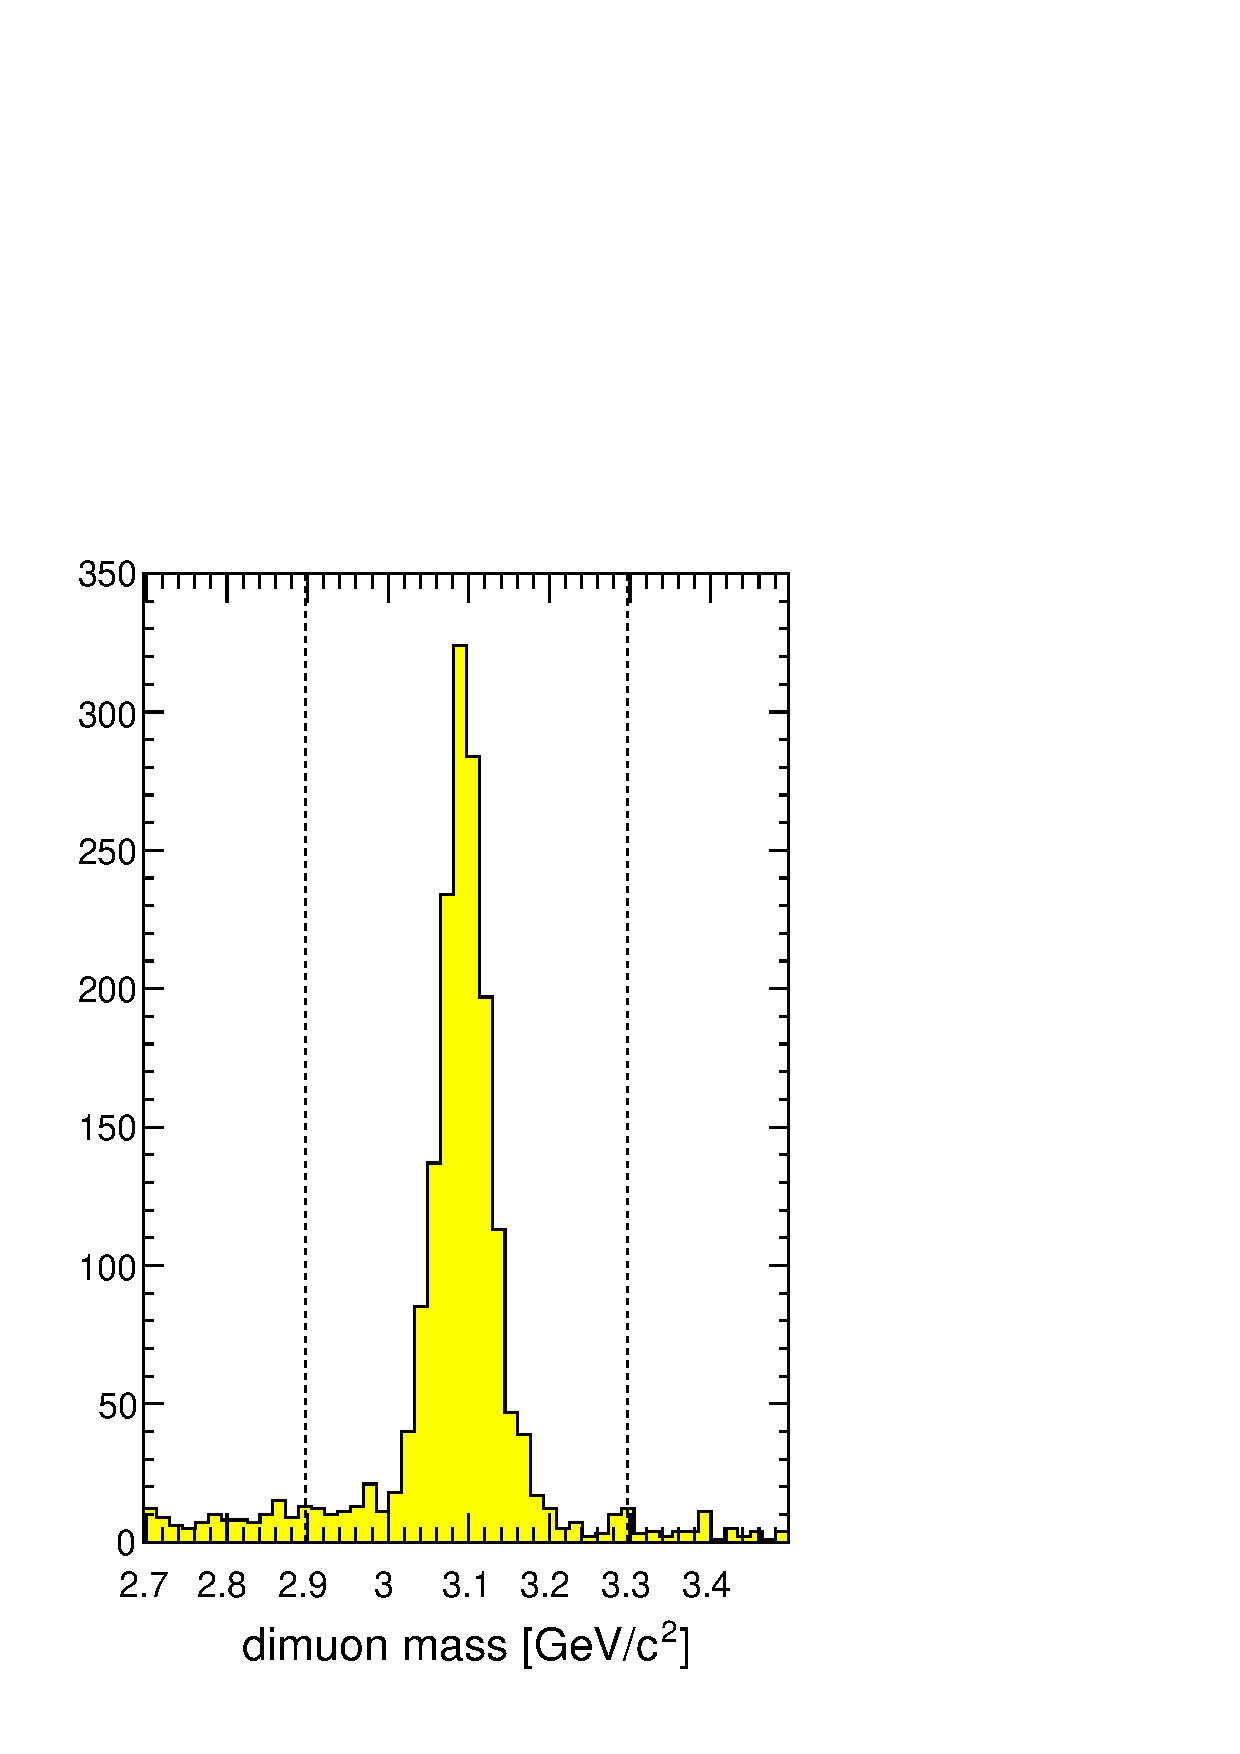
\includegraphics[width=\linewidth]{nocuts_jpsi_mass.pdf}
\end{columns}

\vfill
\begin{columns}
\column{0.5\linewidth}
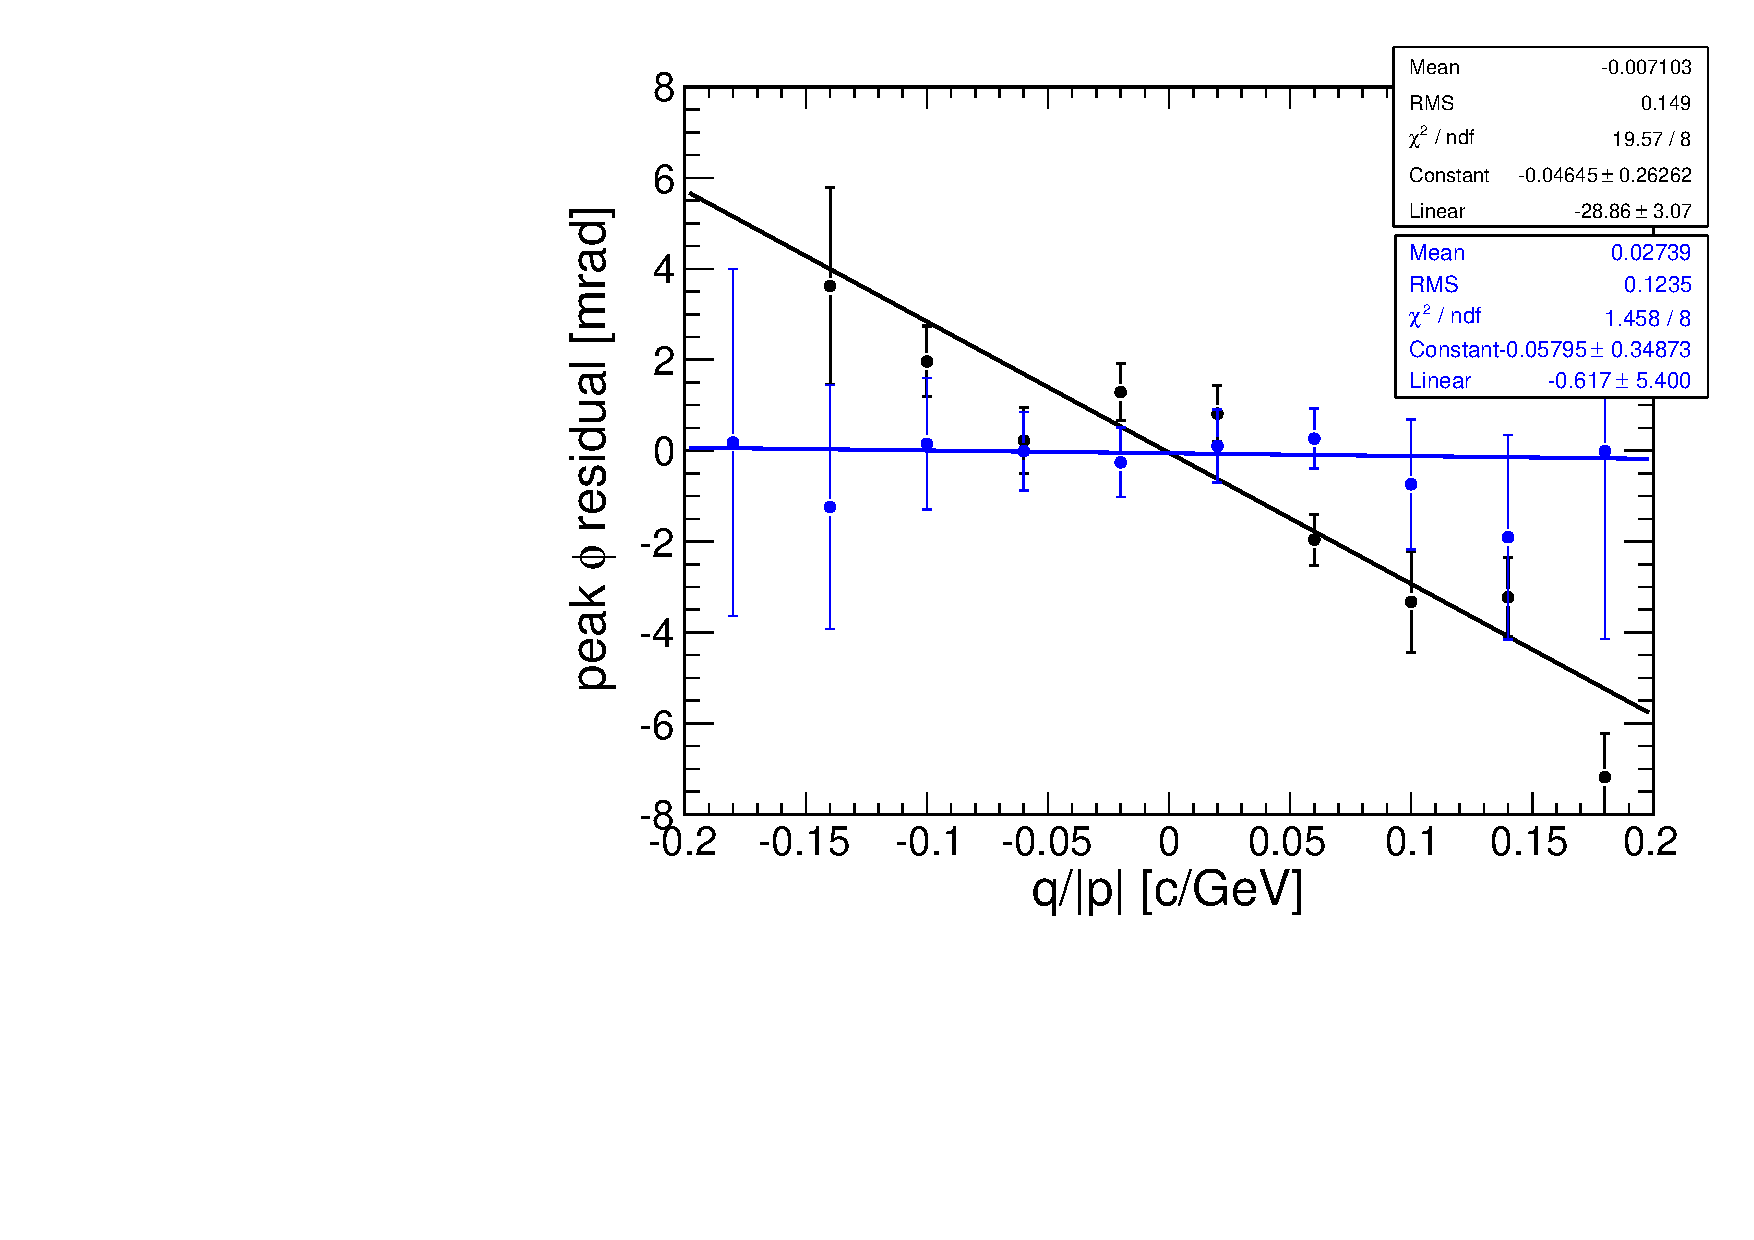
\includegraphics[width=\linewidth]{nocuts_jpsi_qoverpmag.pdf}

\column{0.5\linewidth}
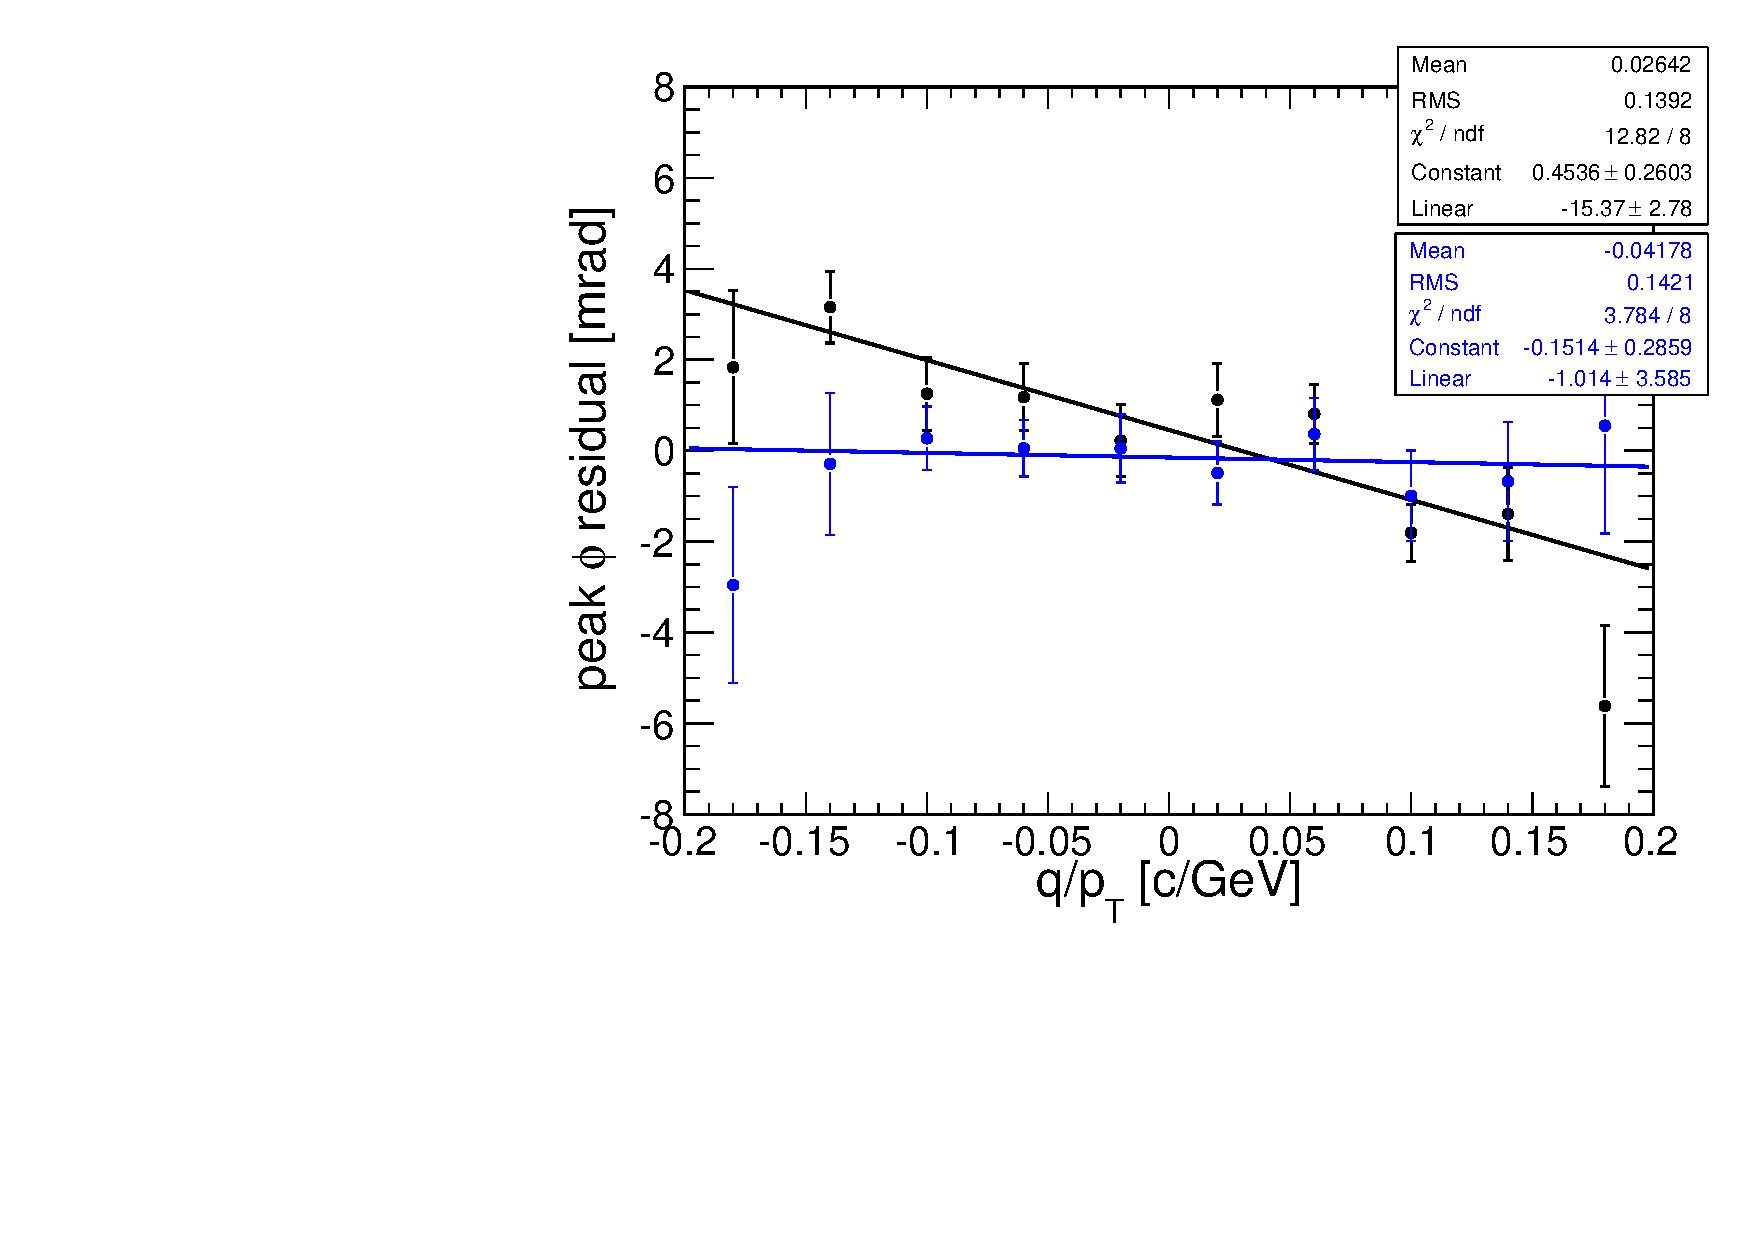
\includegraphics[width=\linewidth]{nocuts_jpsi_qoverpt.pdf}
\end{columns}
\end{frame}

%% \begin{frame}
%% \frametitle{Outline}
%% \begin{itemize}\setlength{\itemsep}{0.75 cm}
%% \item 
%% \end{itemize}
%% %% \hspace{-0.83 cm} \textcolor{darkblue}{\Large Outline2}
%% \end{frame}

% \section*{First section}
\begin{frame}
\begin{center}
\Huge \textcolor{blue}{BACKUP}
\end{center}
\end{frame}

\begin{frame}
\frametitle{MB0/1}

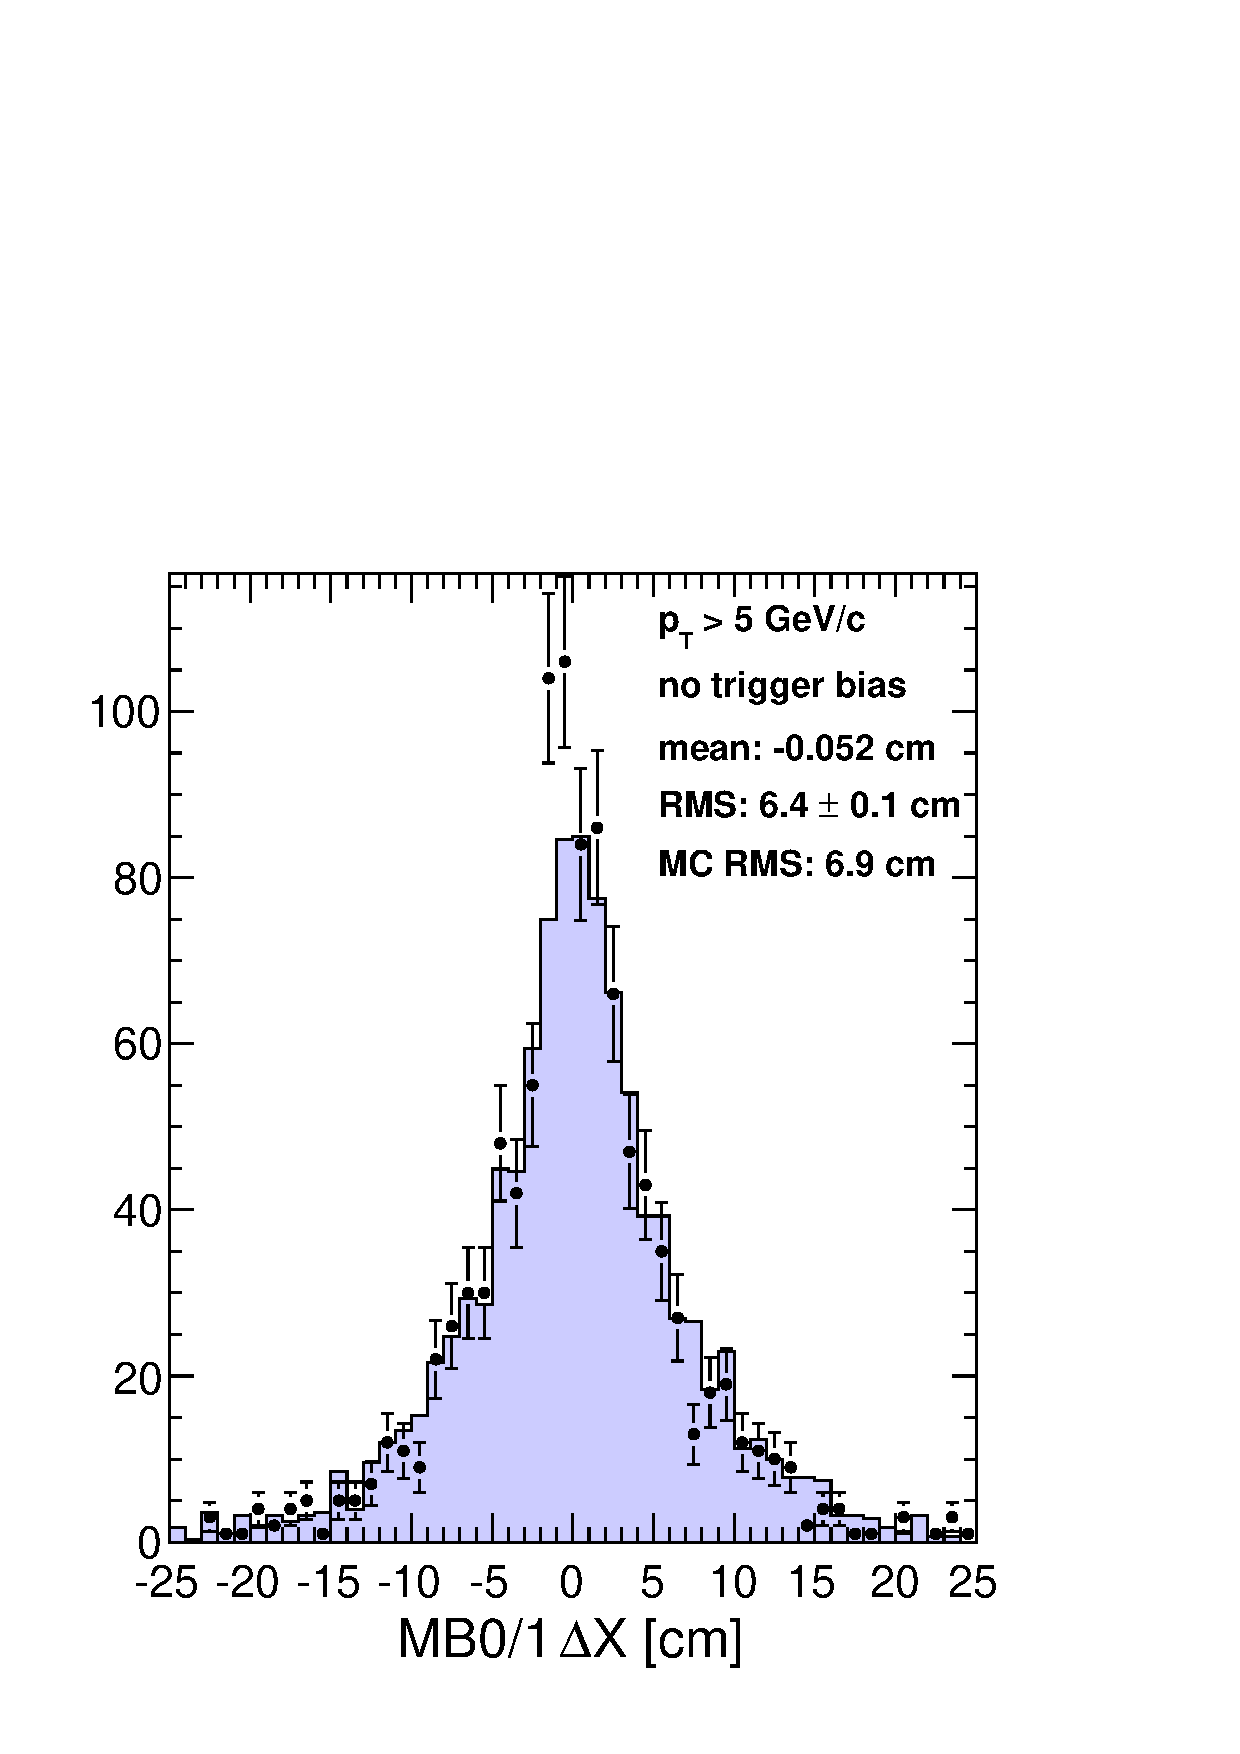
\includegraphics[width=0.24\linewidth]{mb01_X.pdf}
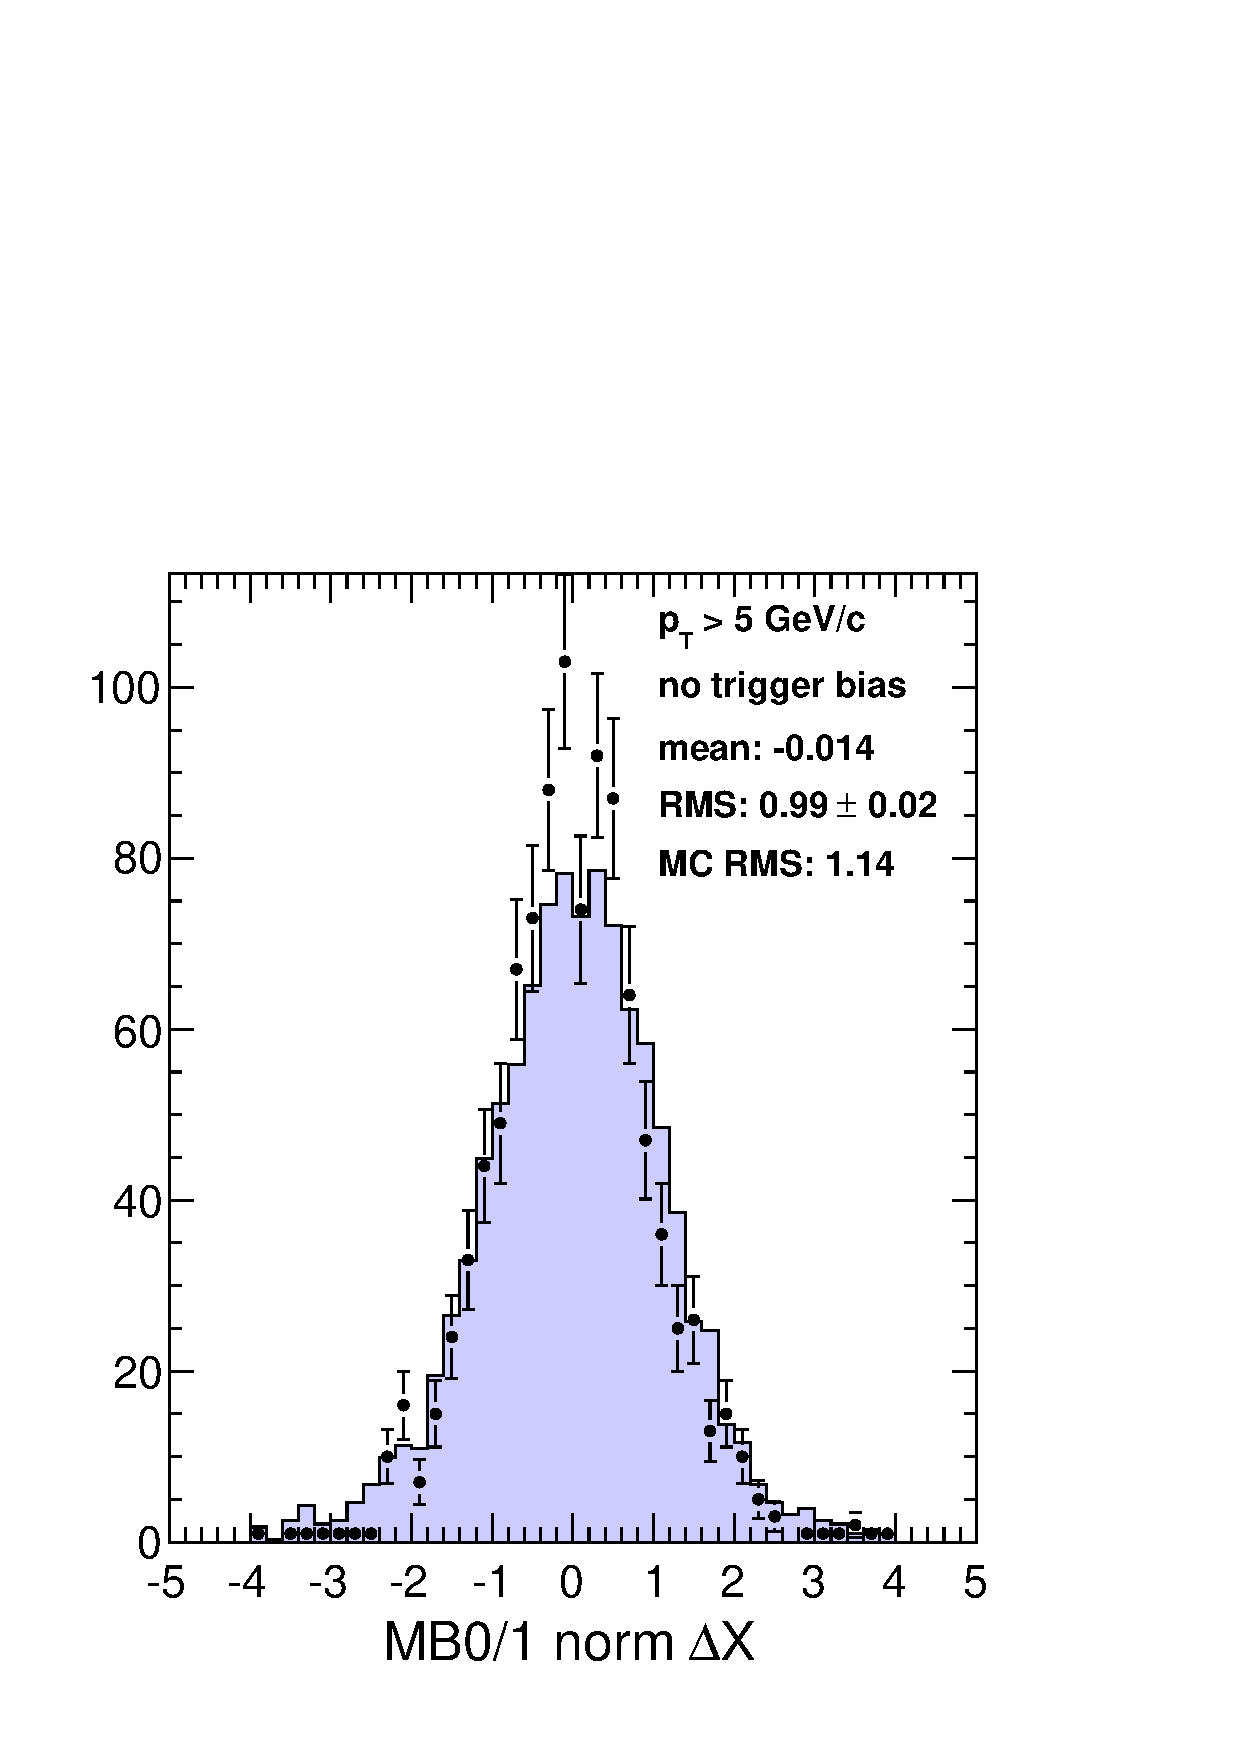
\includegraphics[width=0.24\linewidth]{mb01_Xnorm.pdf}
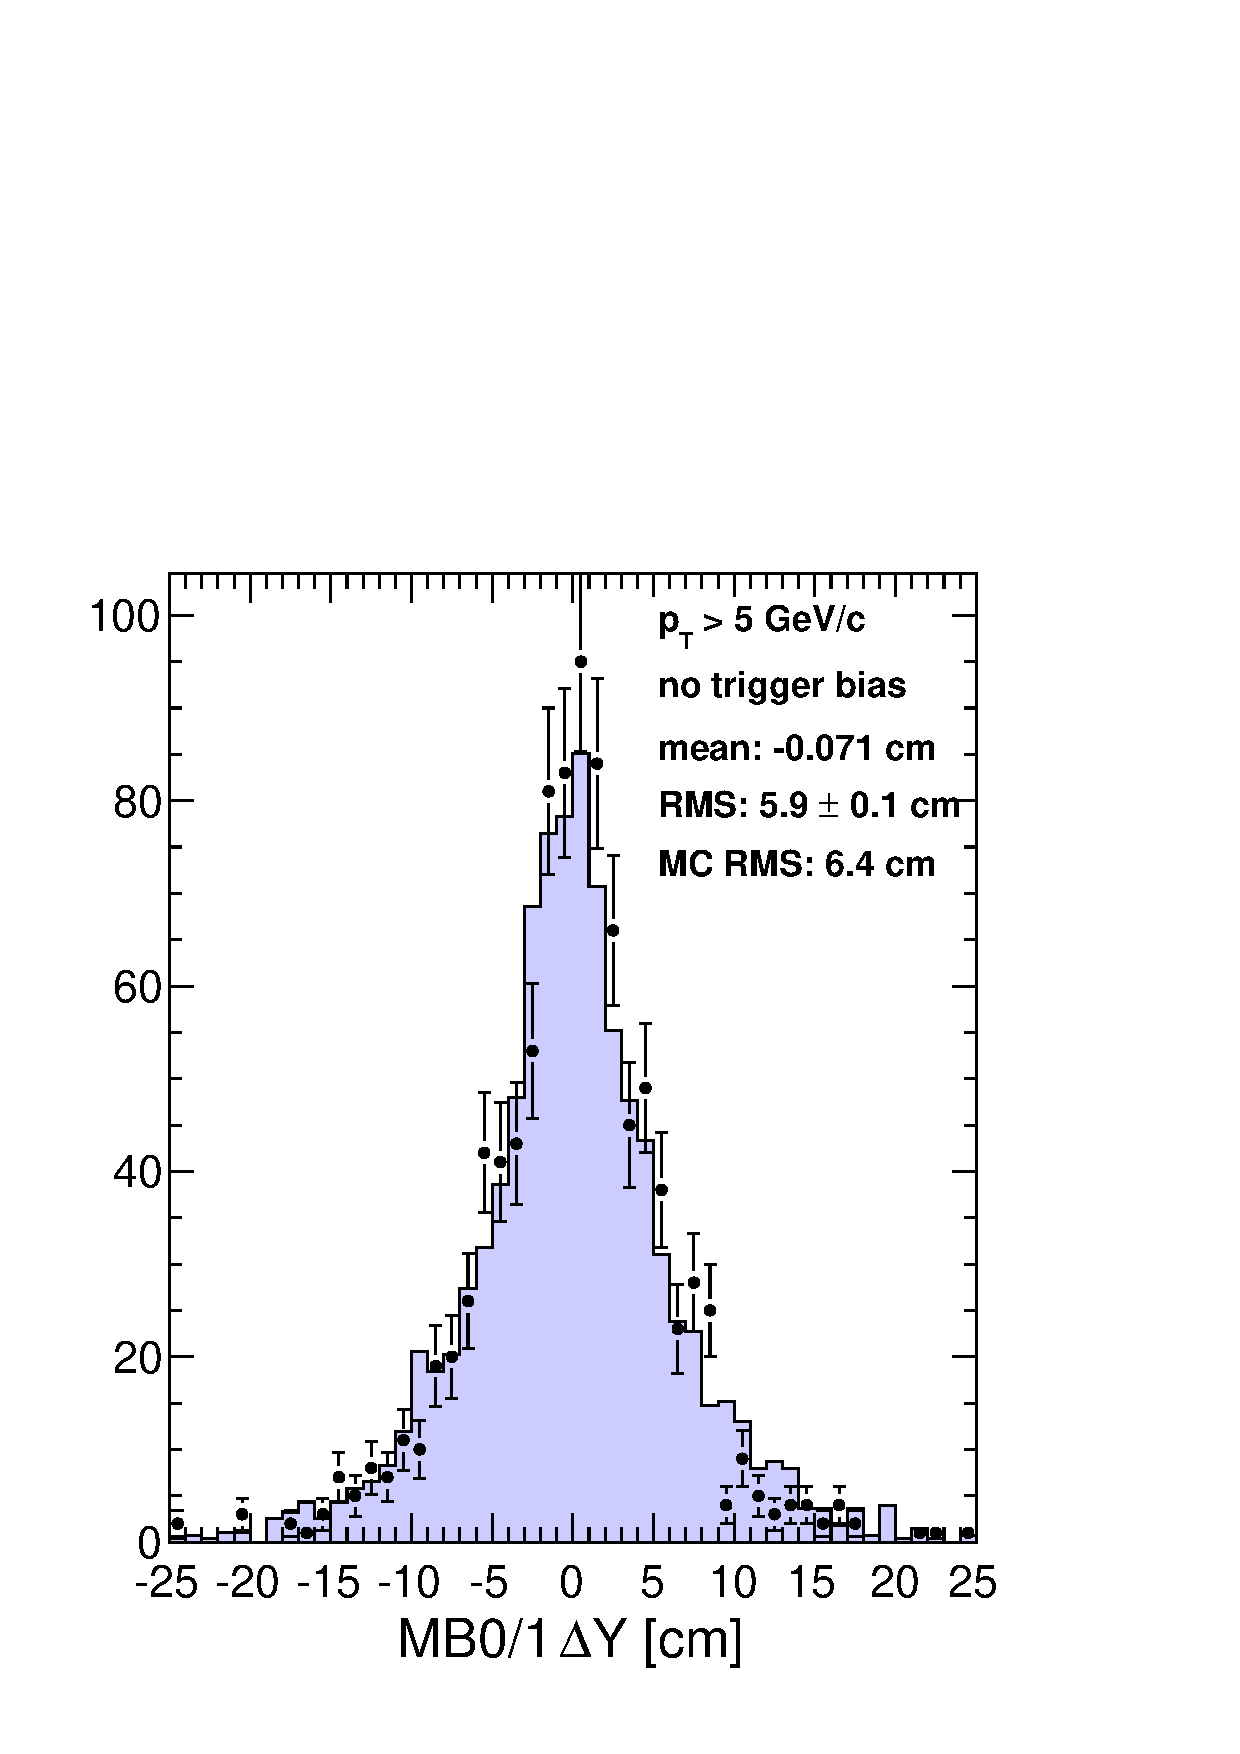
\includegraphics[width=0.24\linewidth]{mb01_Y.pdf}
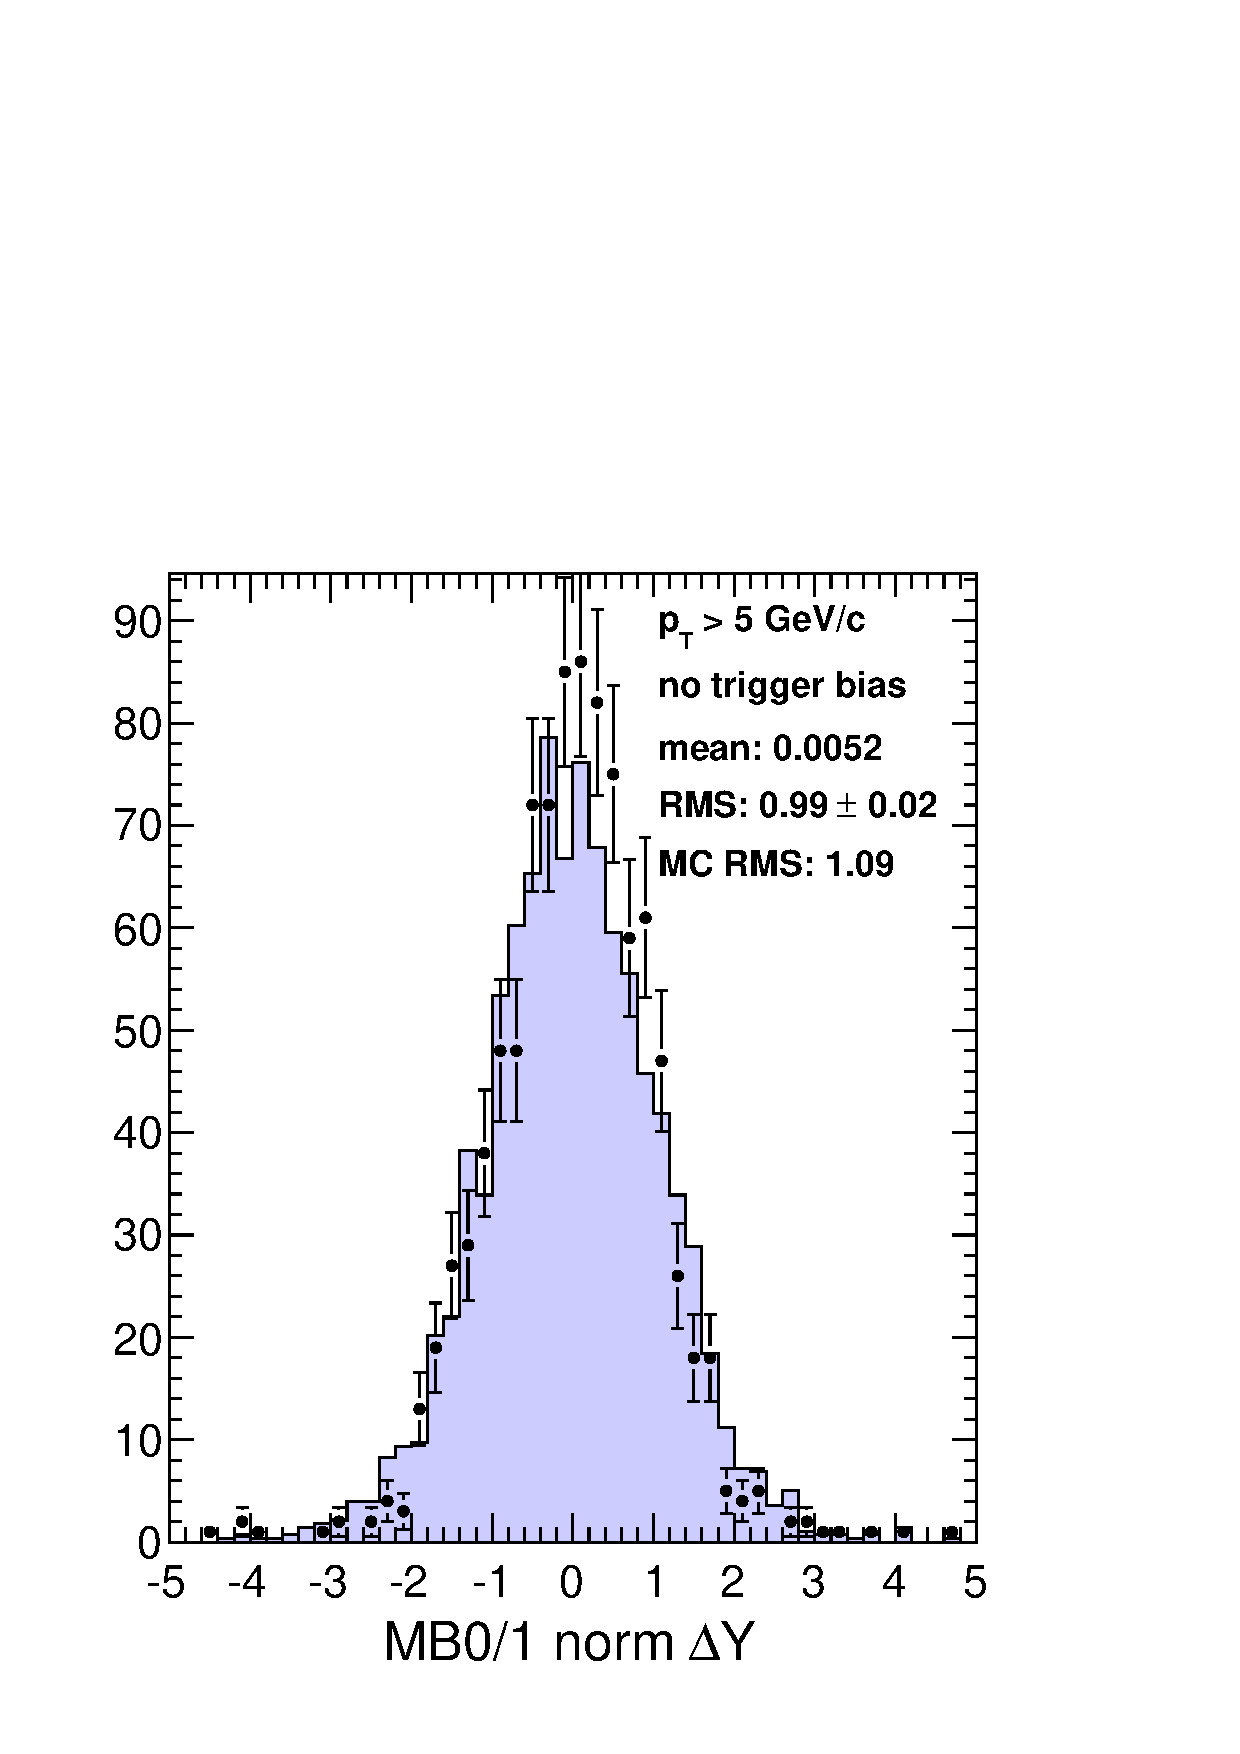
\includegraphics[width=0.24\linewidth]{mb01_Ynorm.pdf}

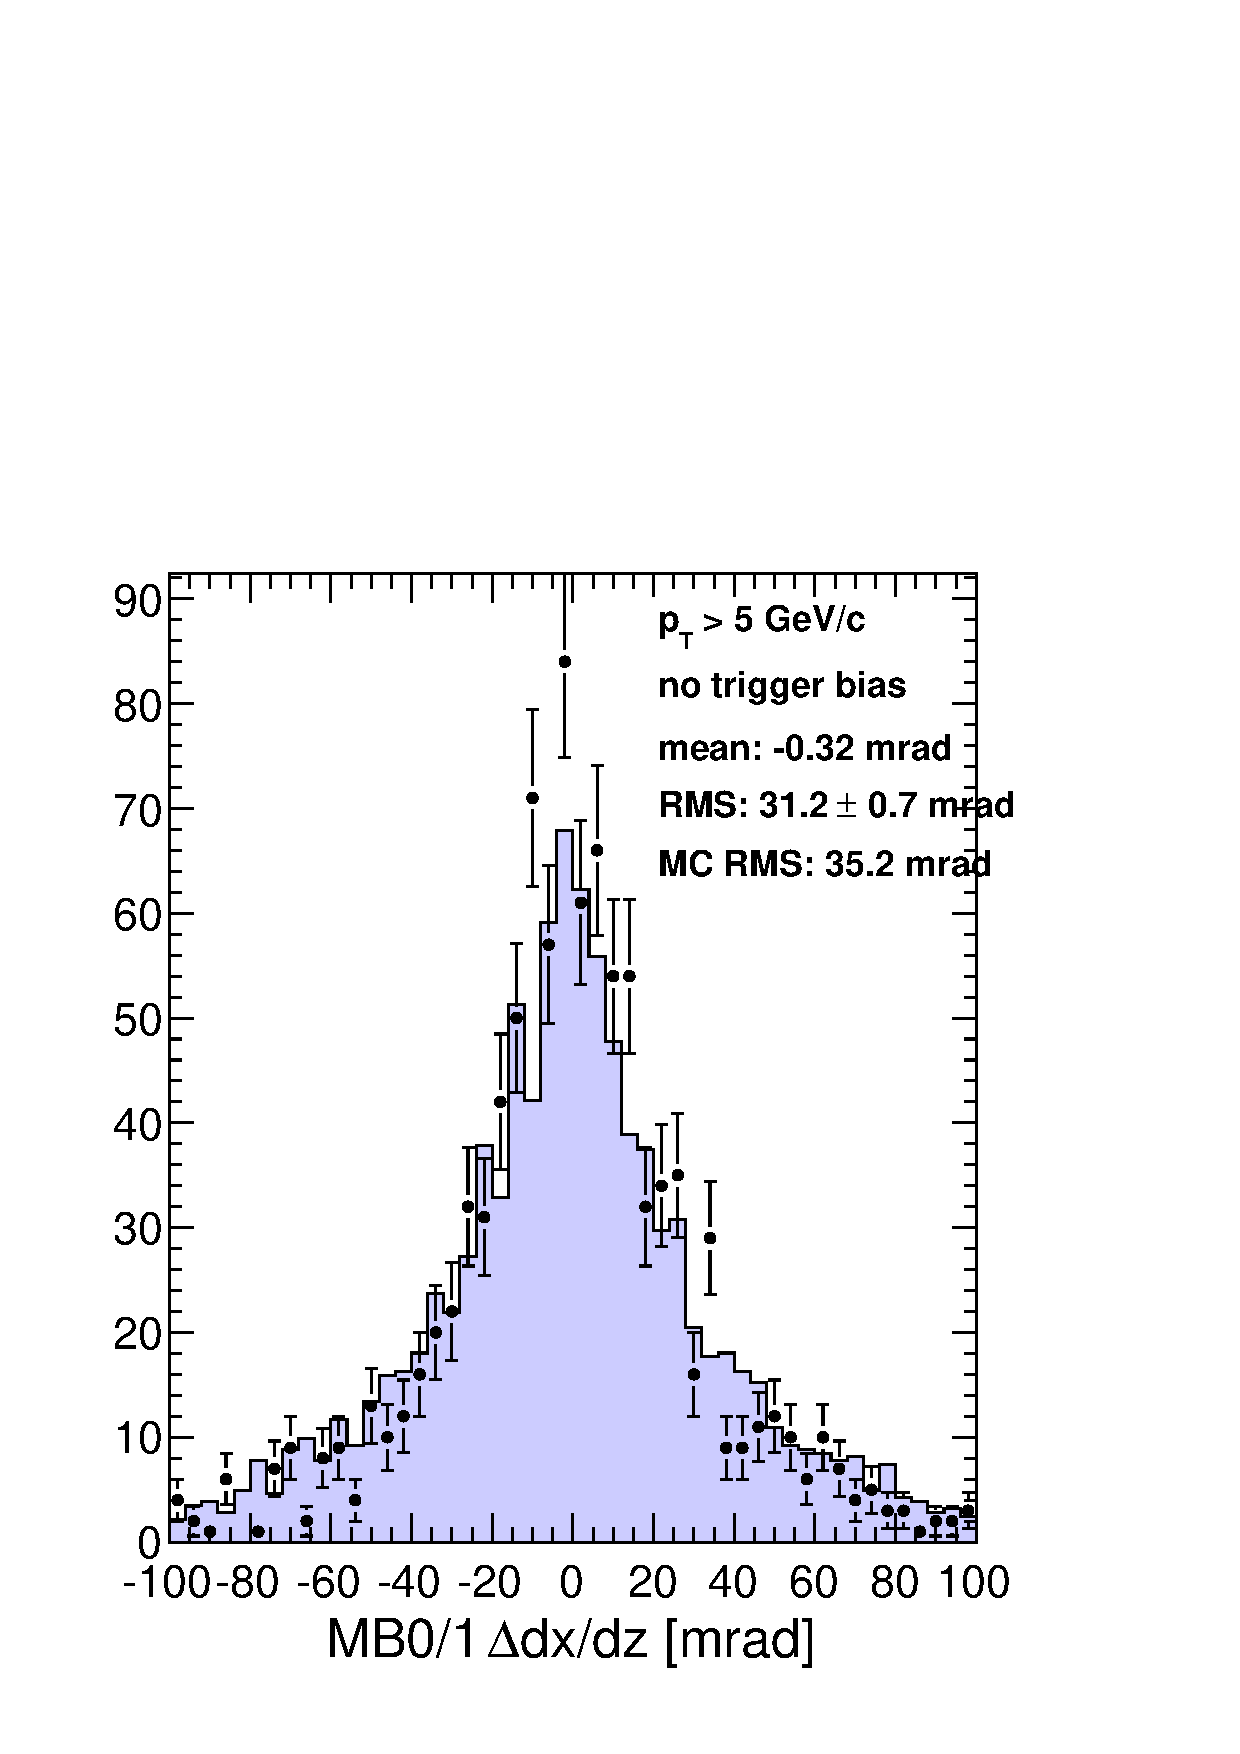
\includegraphics[width=0.24\linewidth]{mb01_dXdZ.pdf}
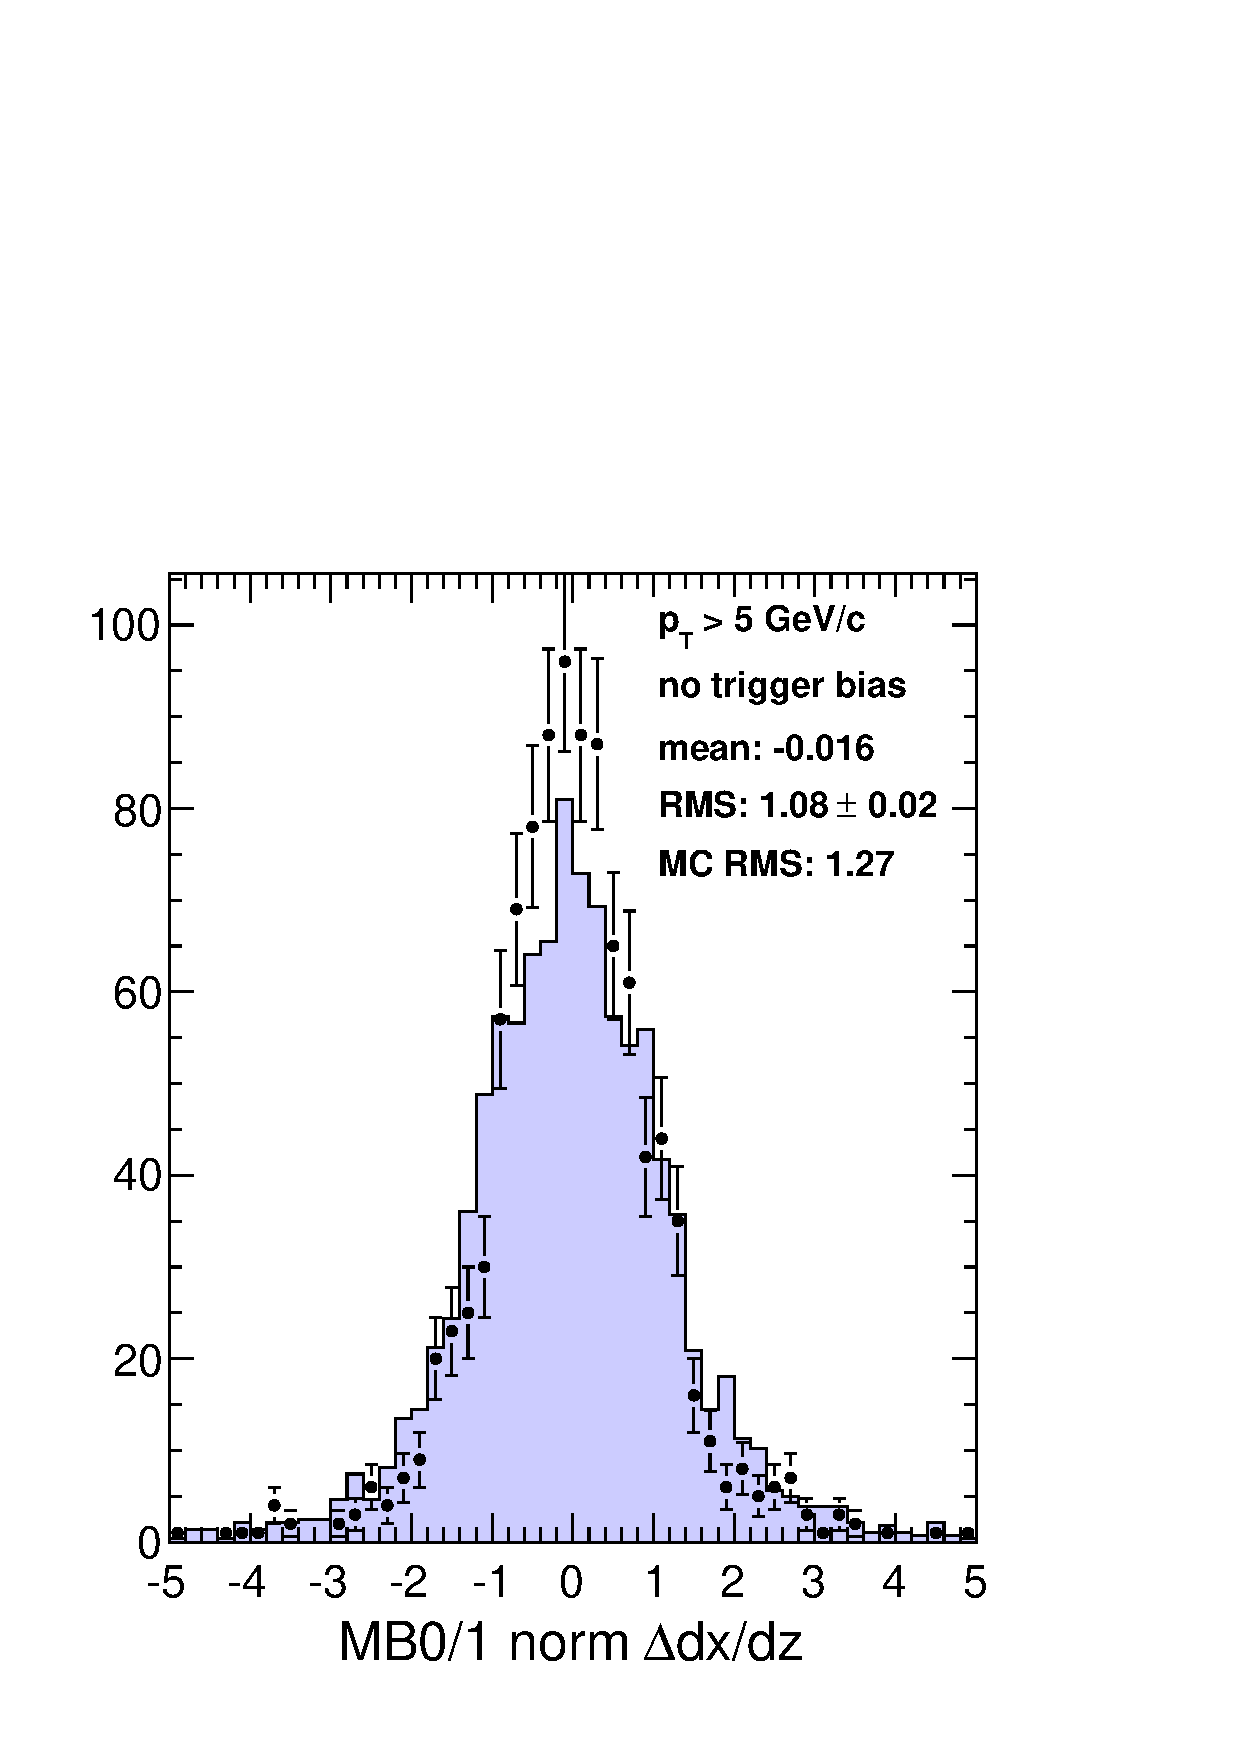
\includegraphics[width=0.24\linewidth]{mb01_dXdZnorm.pdf}
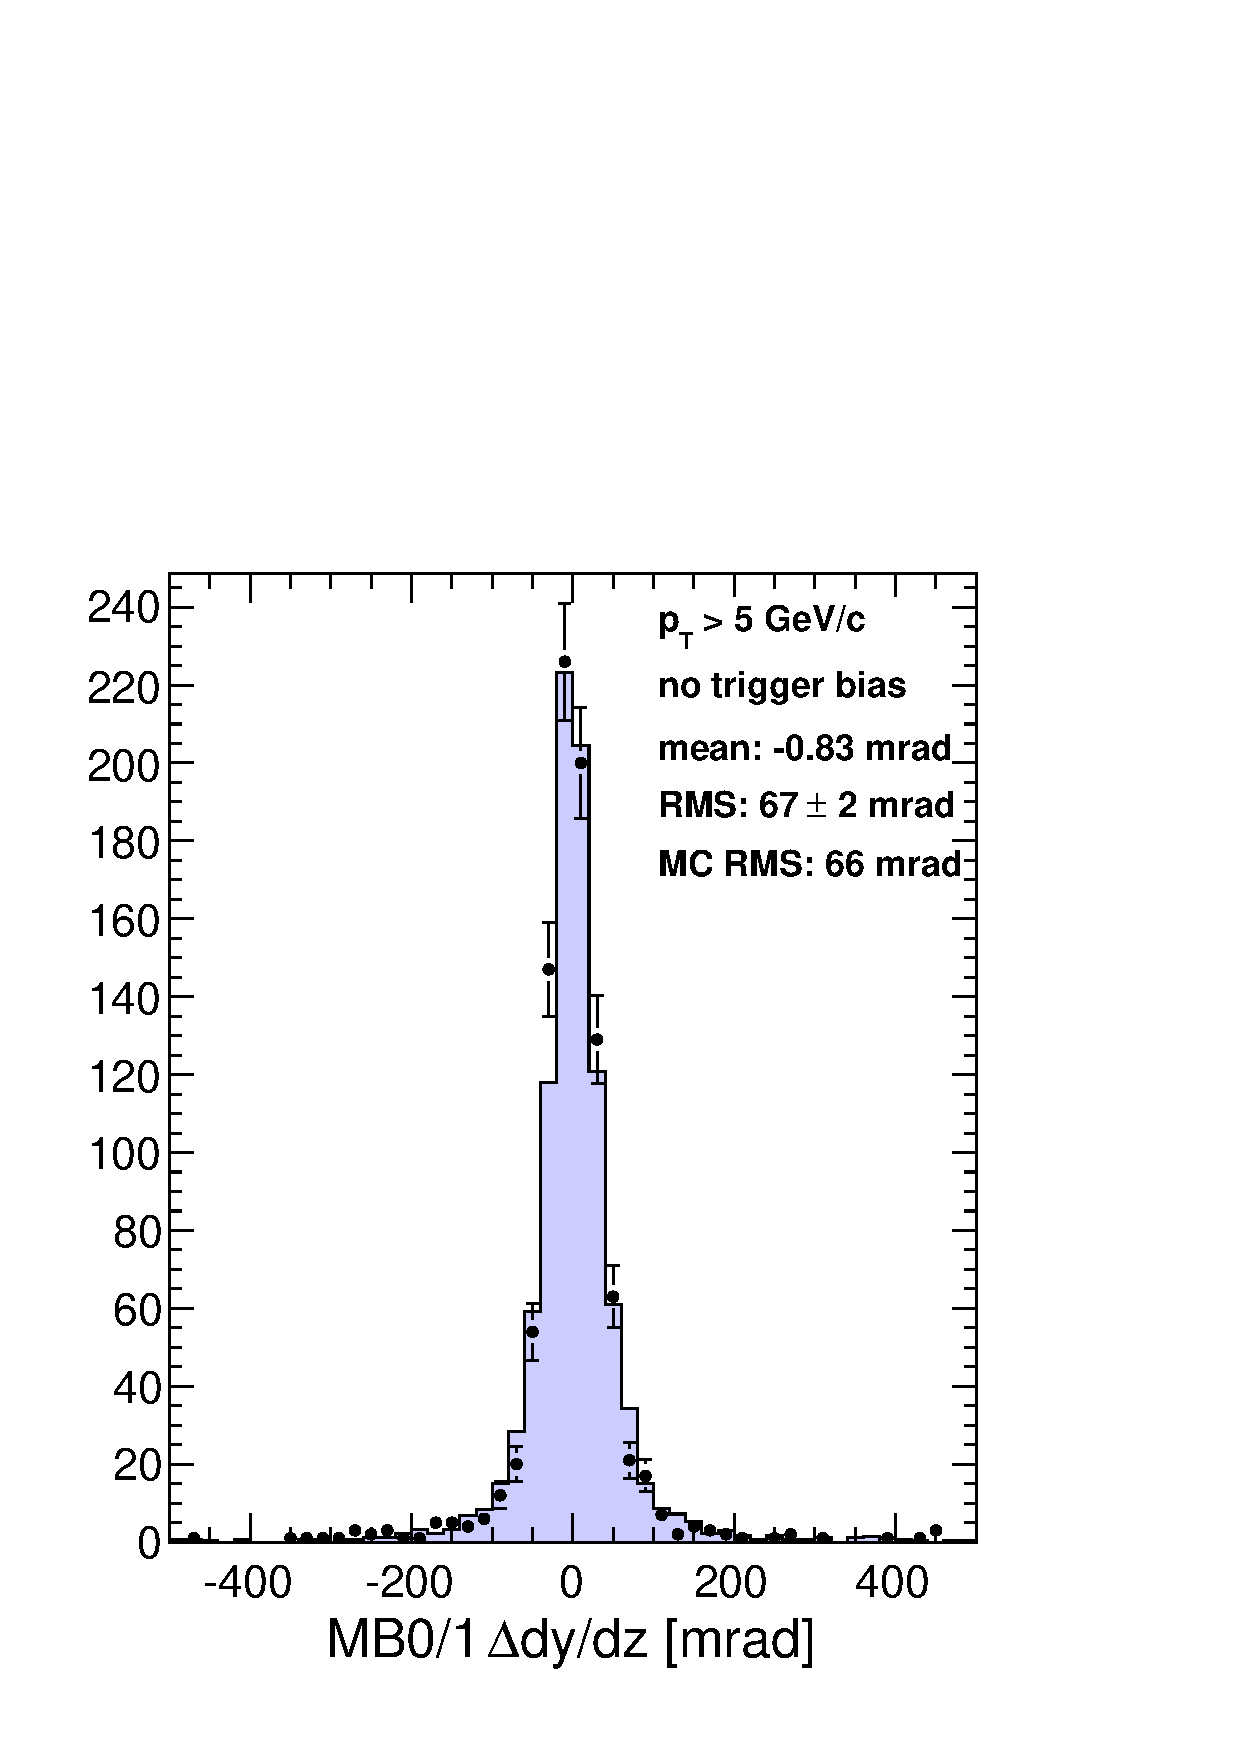
\includegraphics[width=0.24\linewidth]{mb01_dYdZ.pdf}
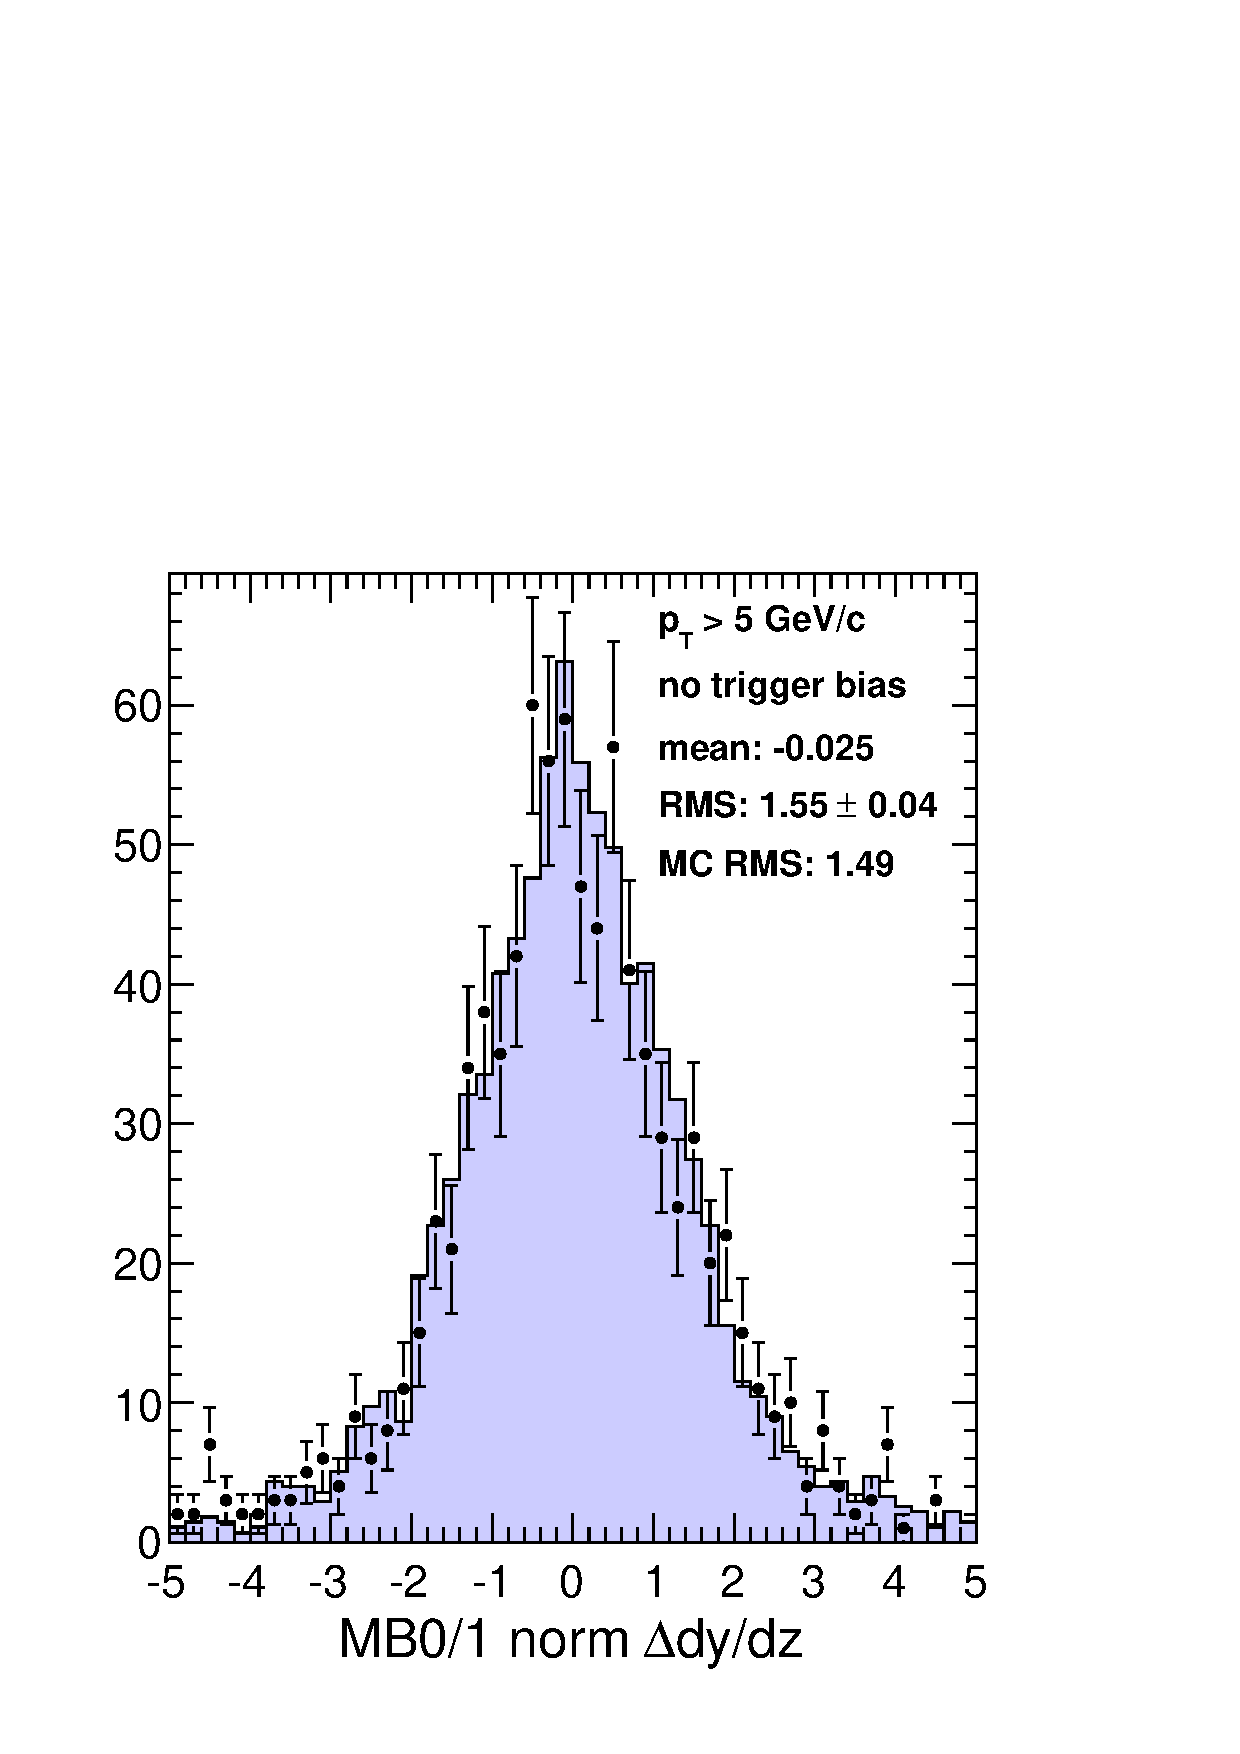
\includegraphics[width=0.24\linewidth]{mb01_dYdZnorm.pdf}
\end{frame}

\begin{frame}
\frametitle{MB0/2}

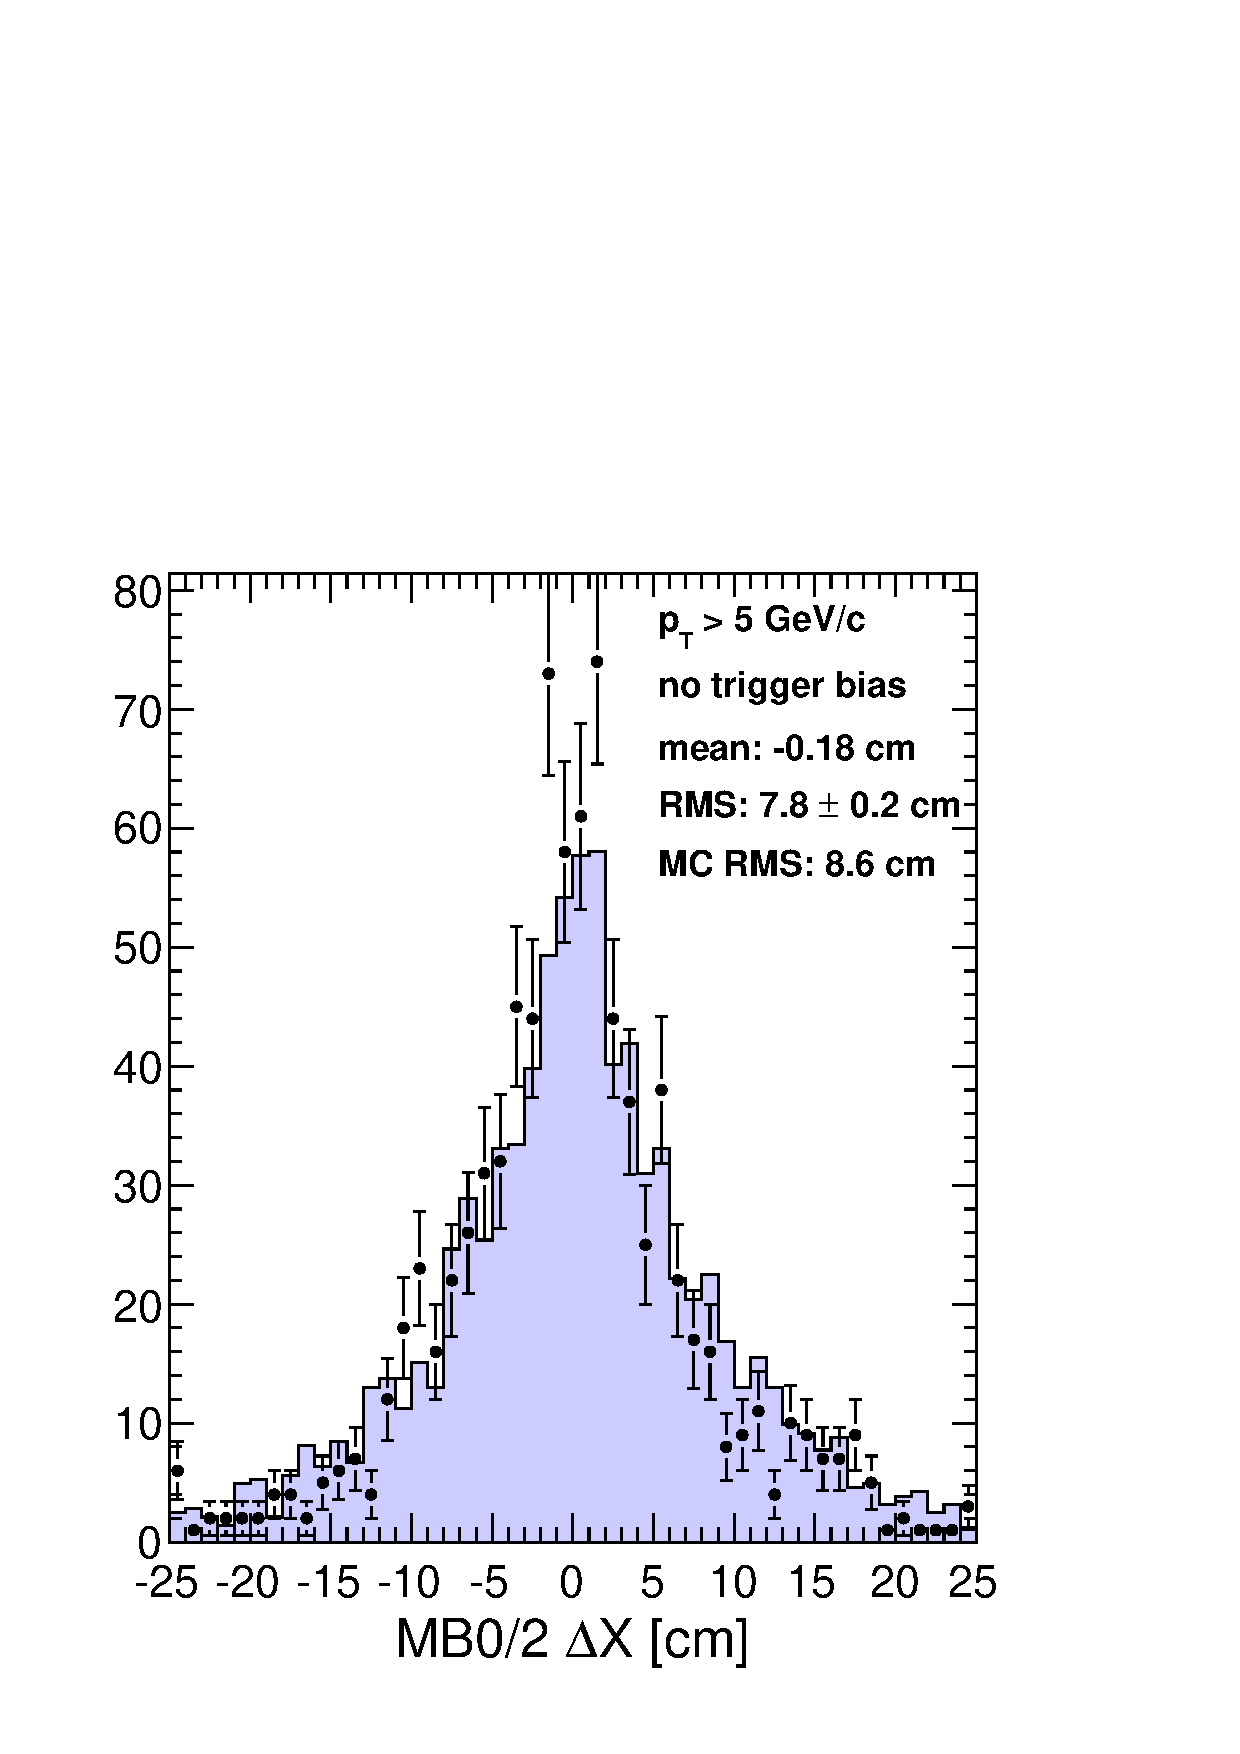
\includegraphics[width=0.24\linewidth]{mb02_X.pdf}
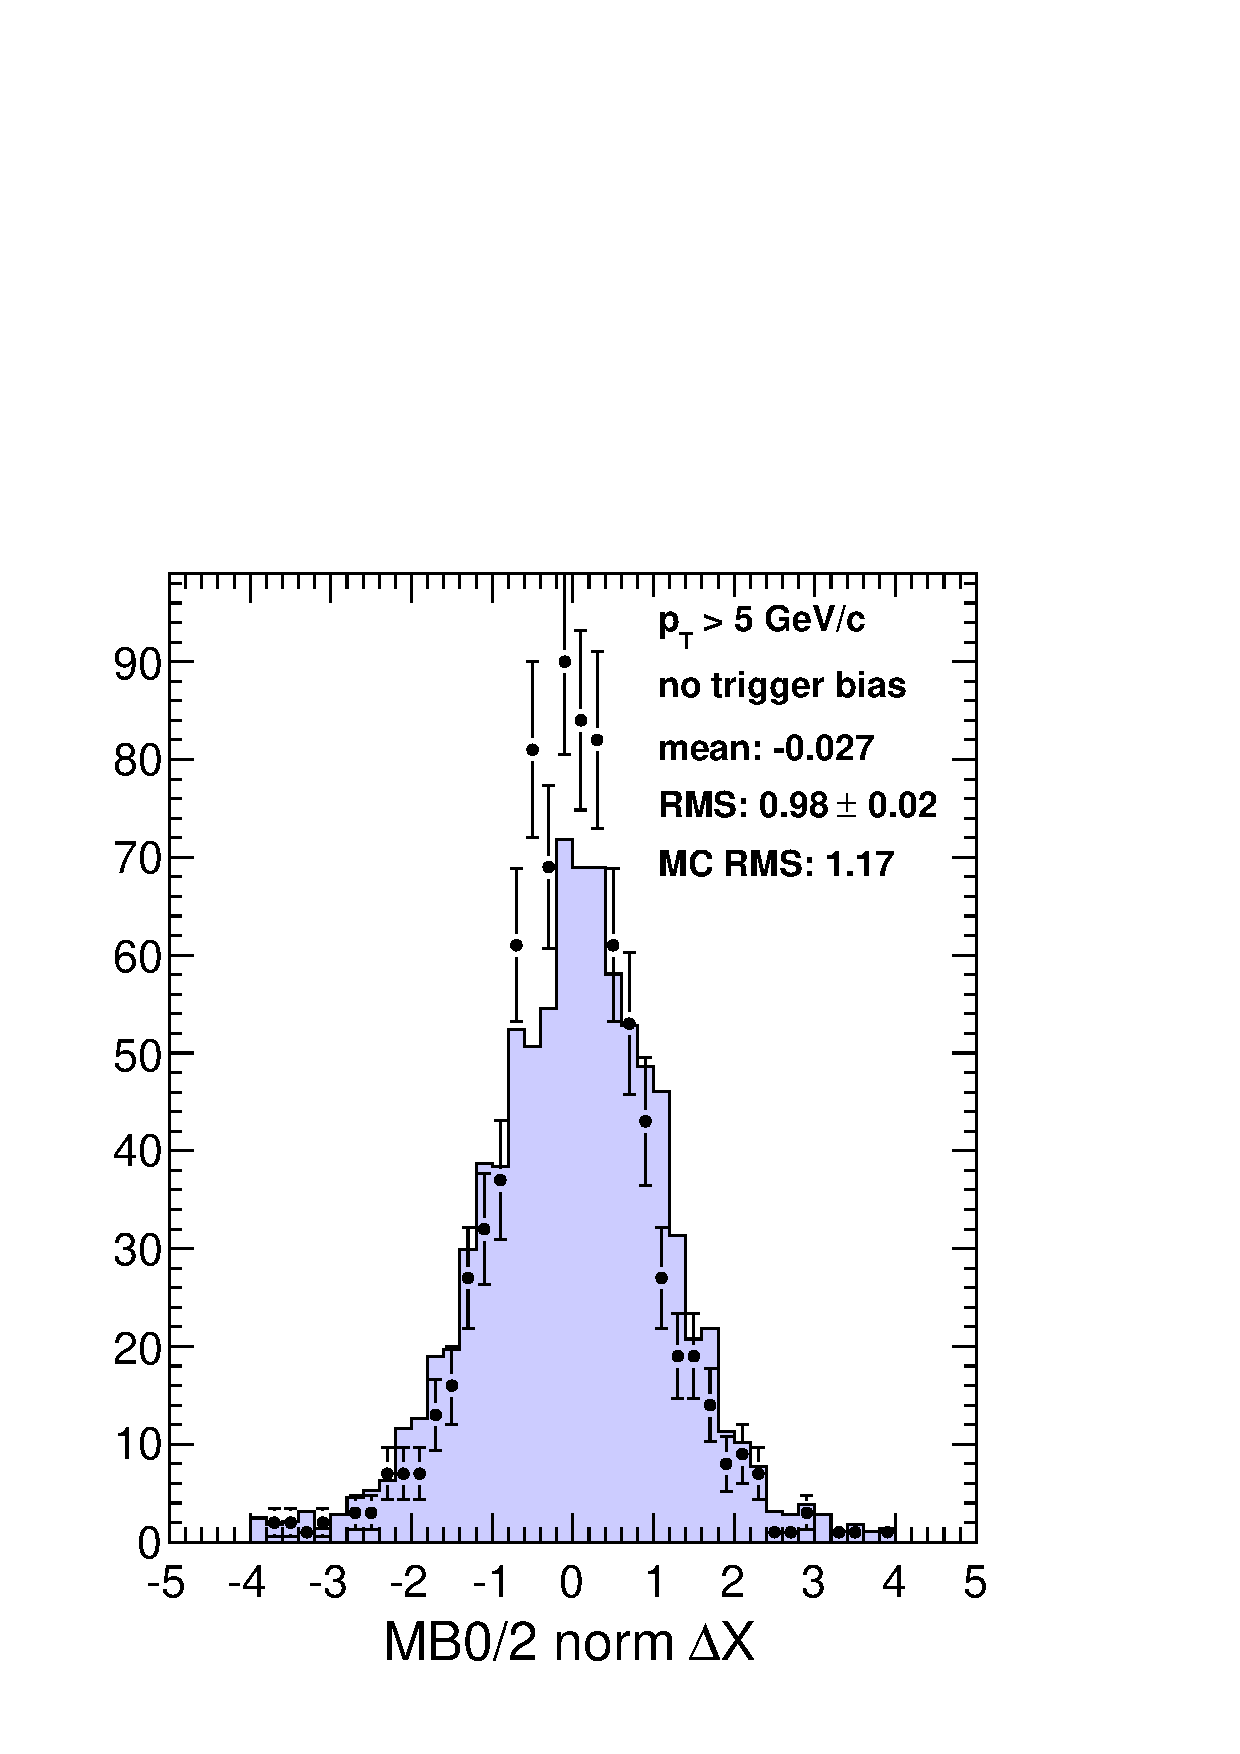
\includegraphics[width=0.24\linewidth]{mb02_Xnorm.pdf}
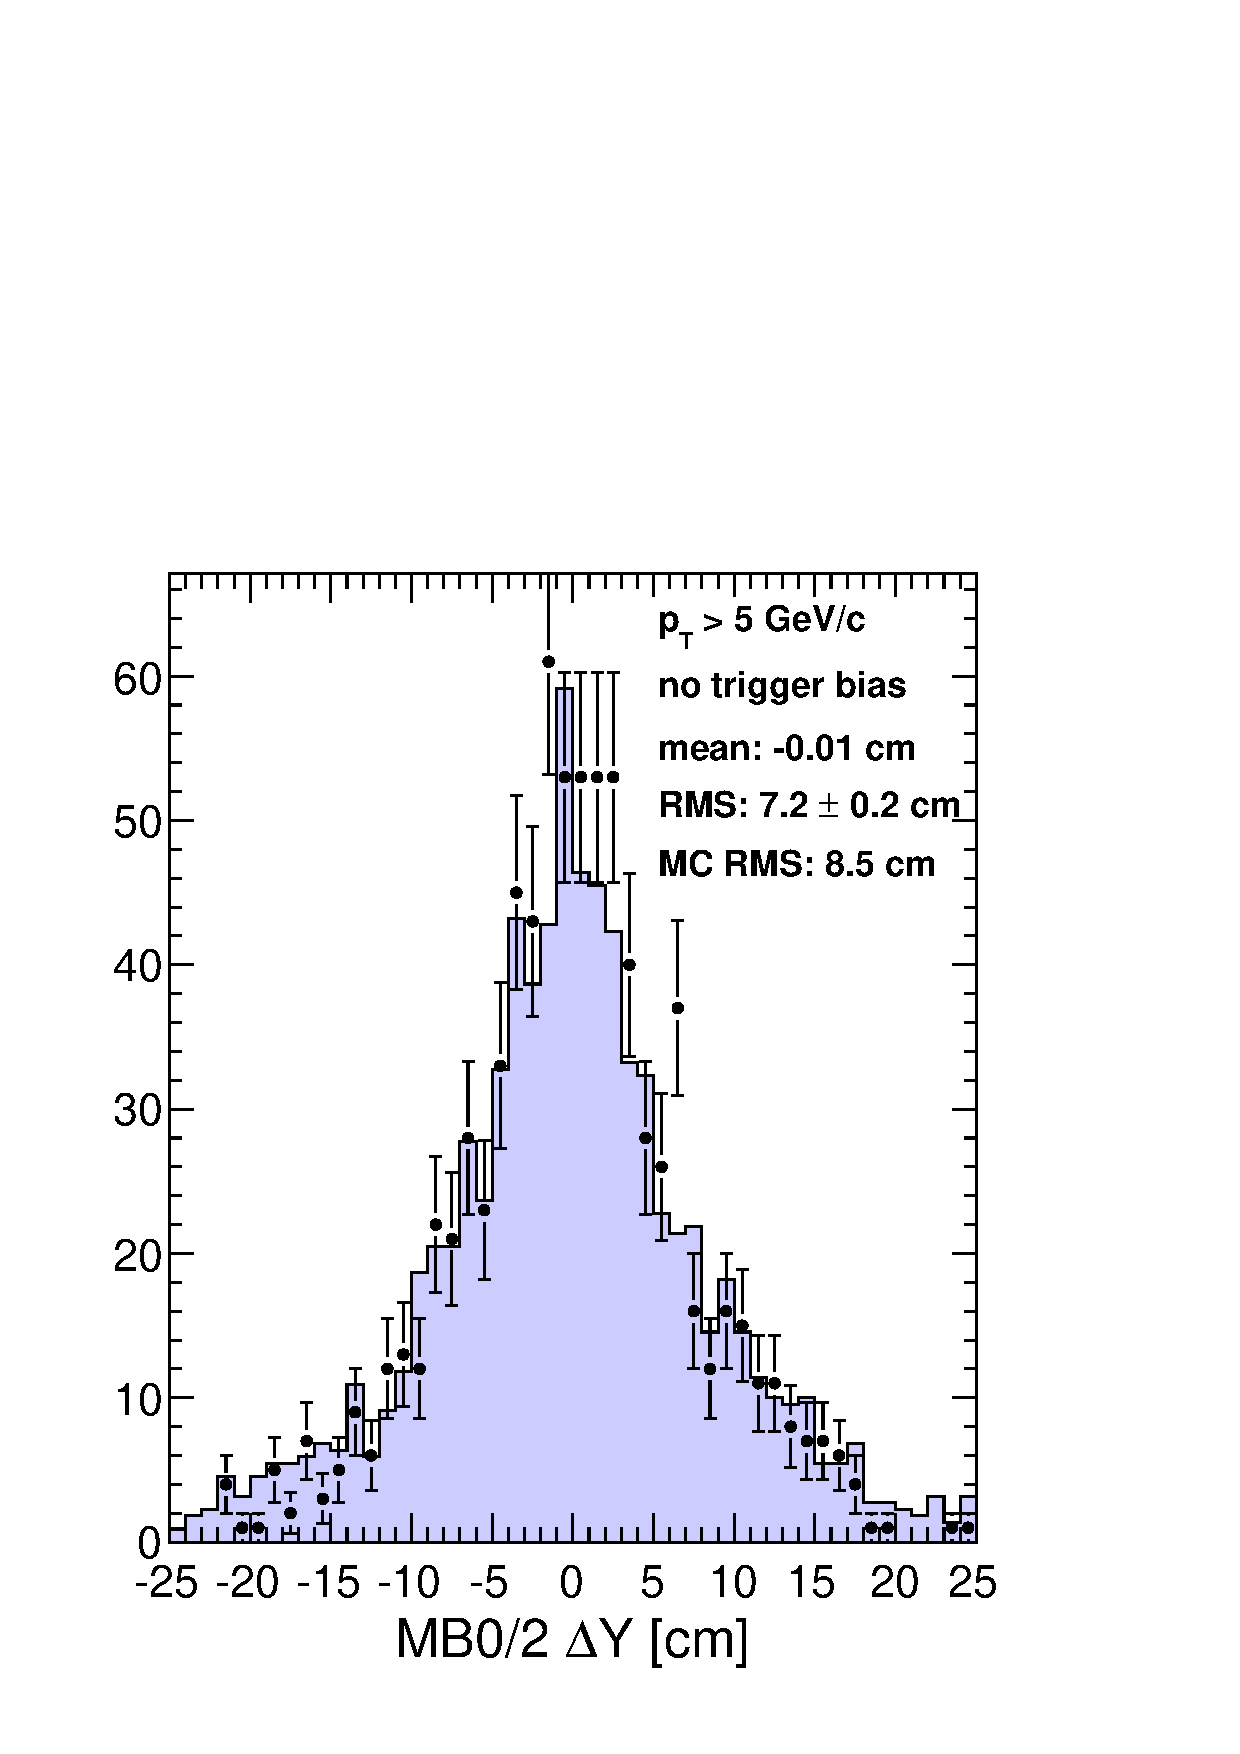
\includegraphics[width=0.24\linewidth]{mb02_Y.pdf}
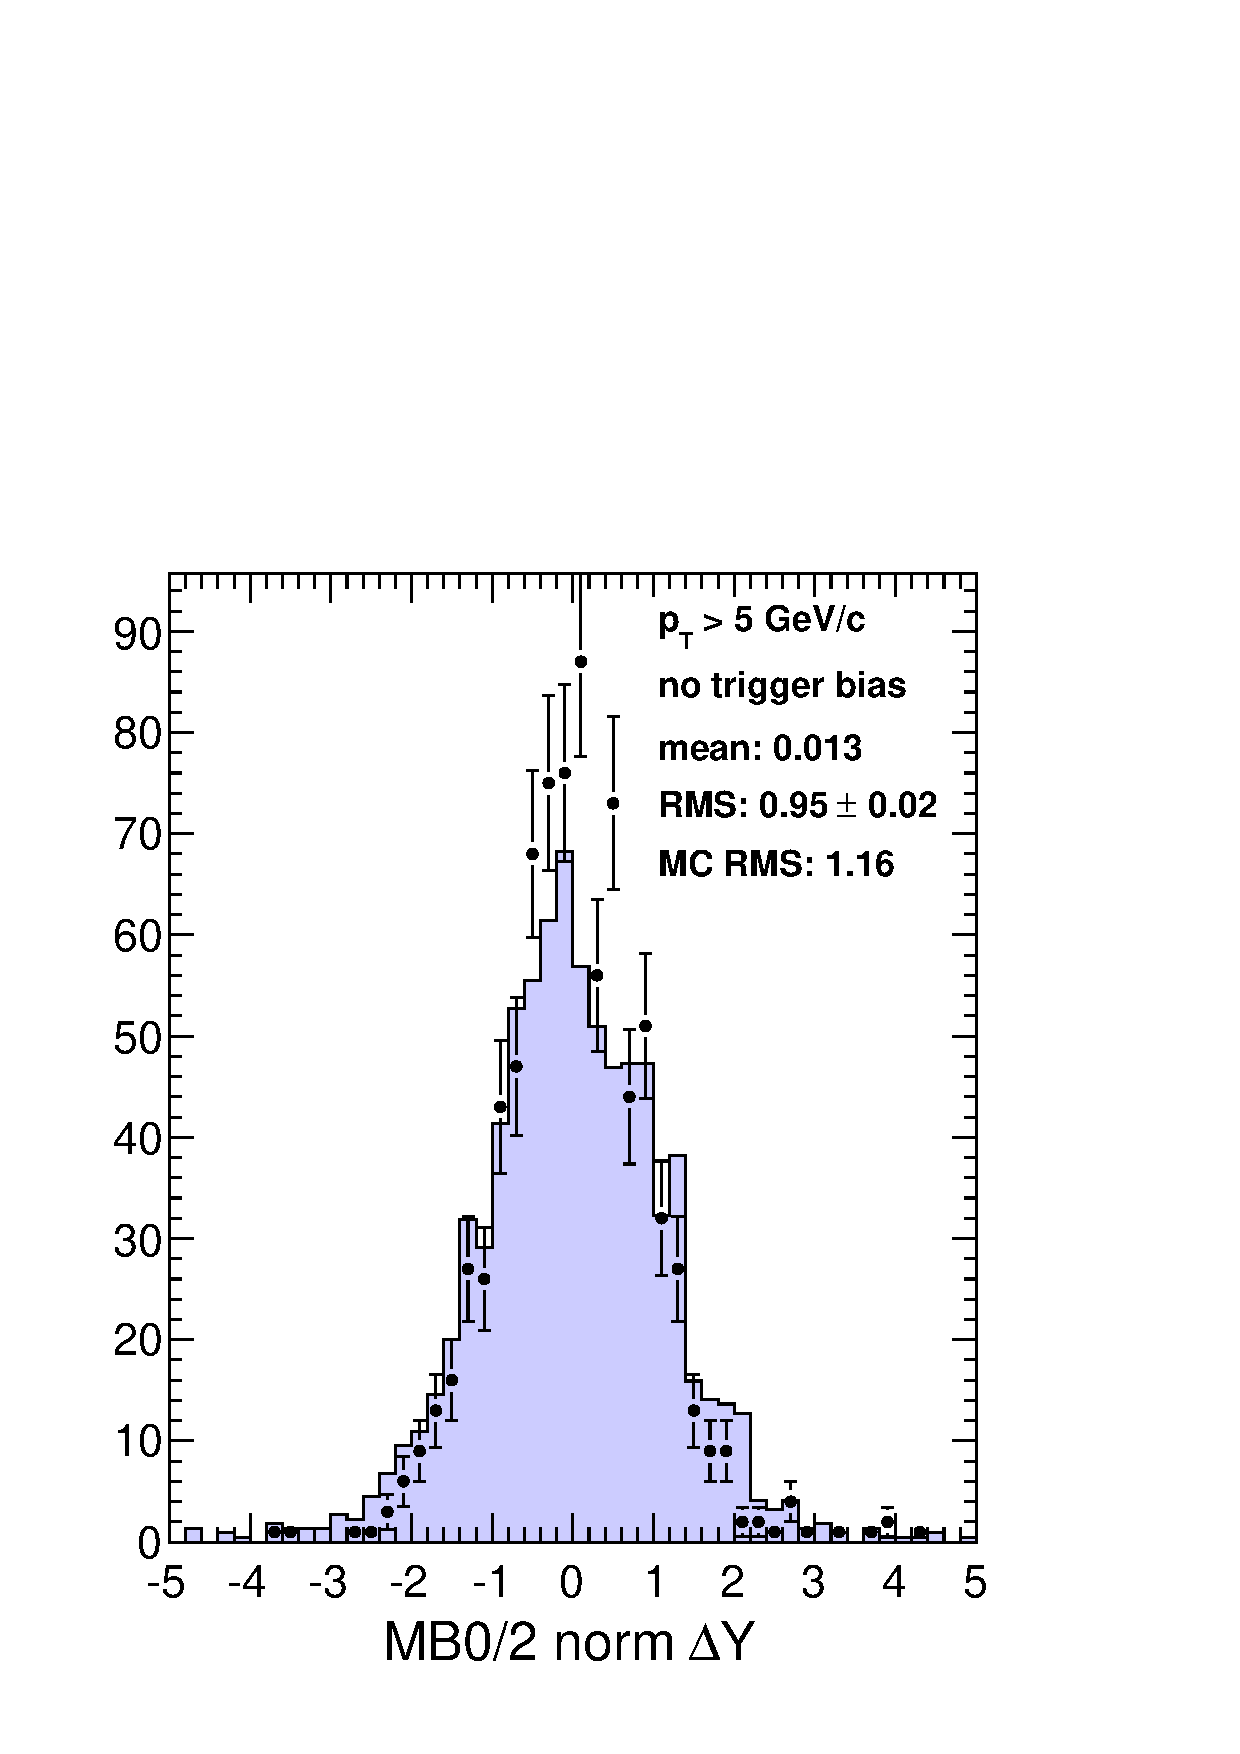
\includegraphics[width=0.24\linewidth]{mb02_Ynorm.pdf}

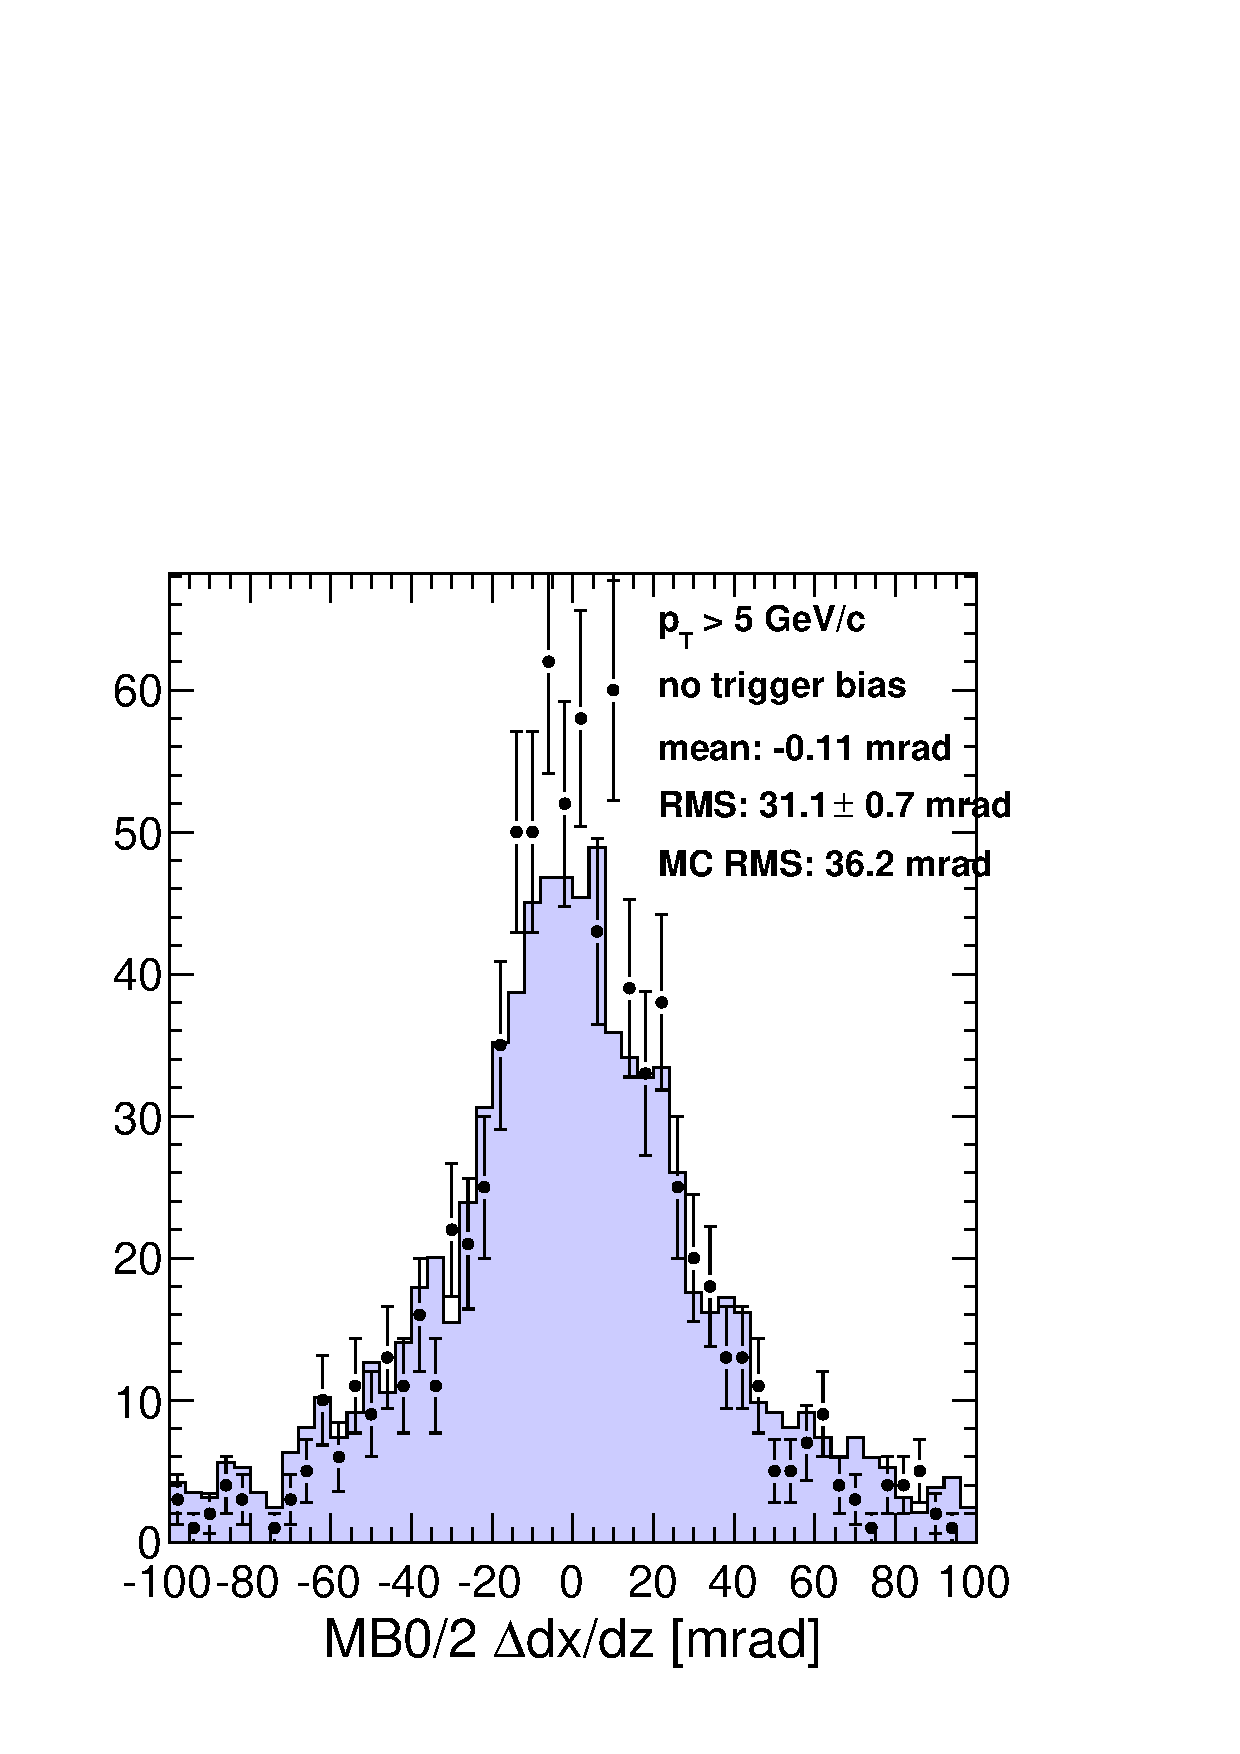
\includegraphics[width=0.24\linewidth]{mb02_dXdZ.pdf}
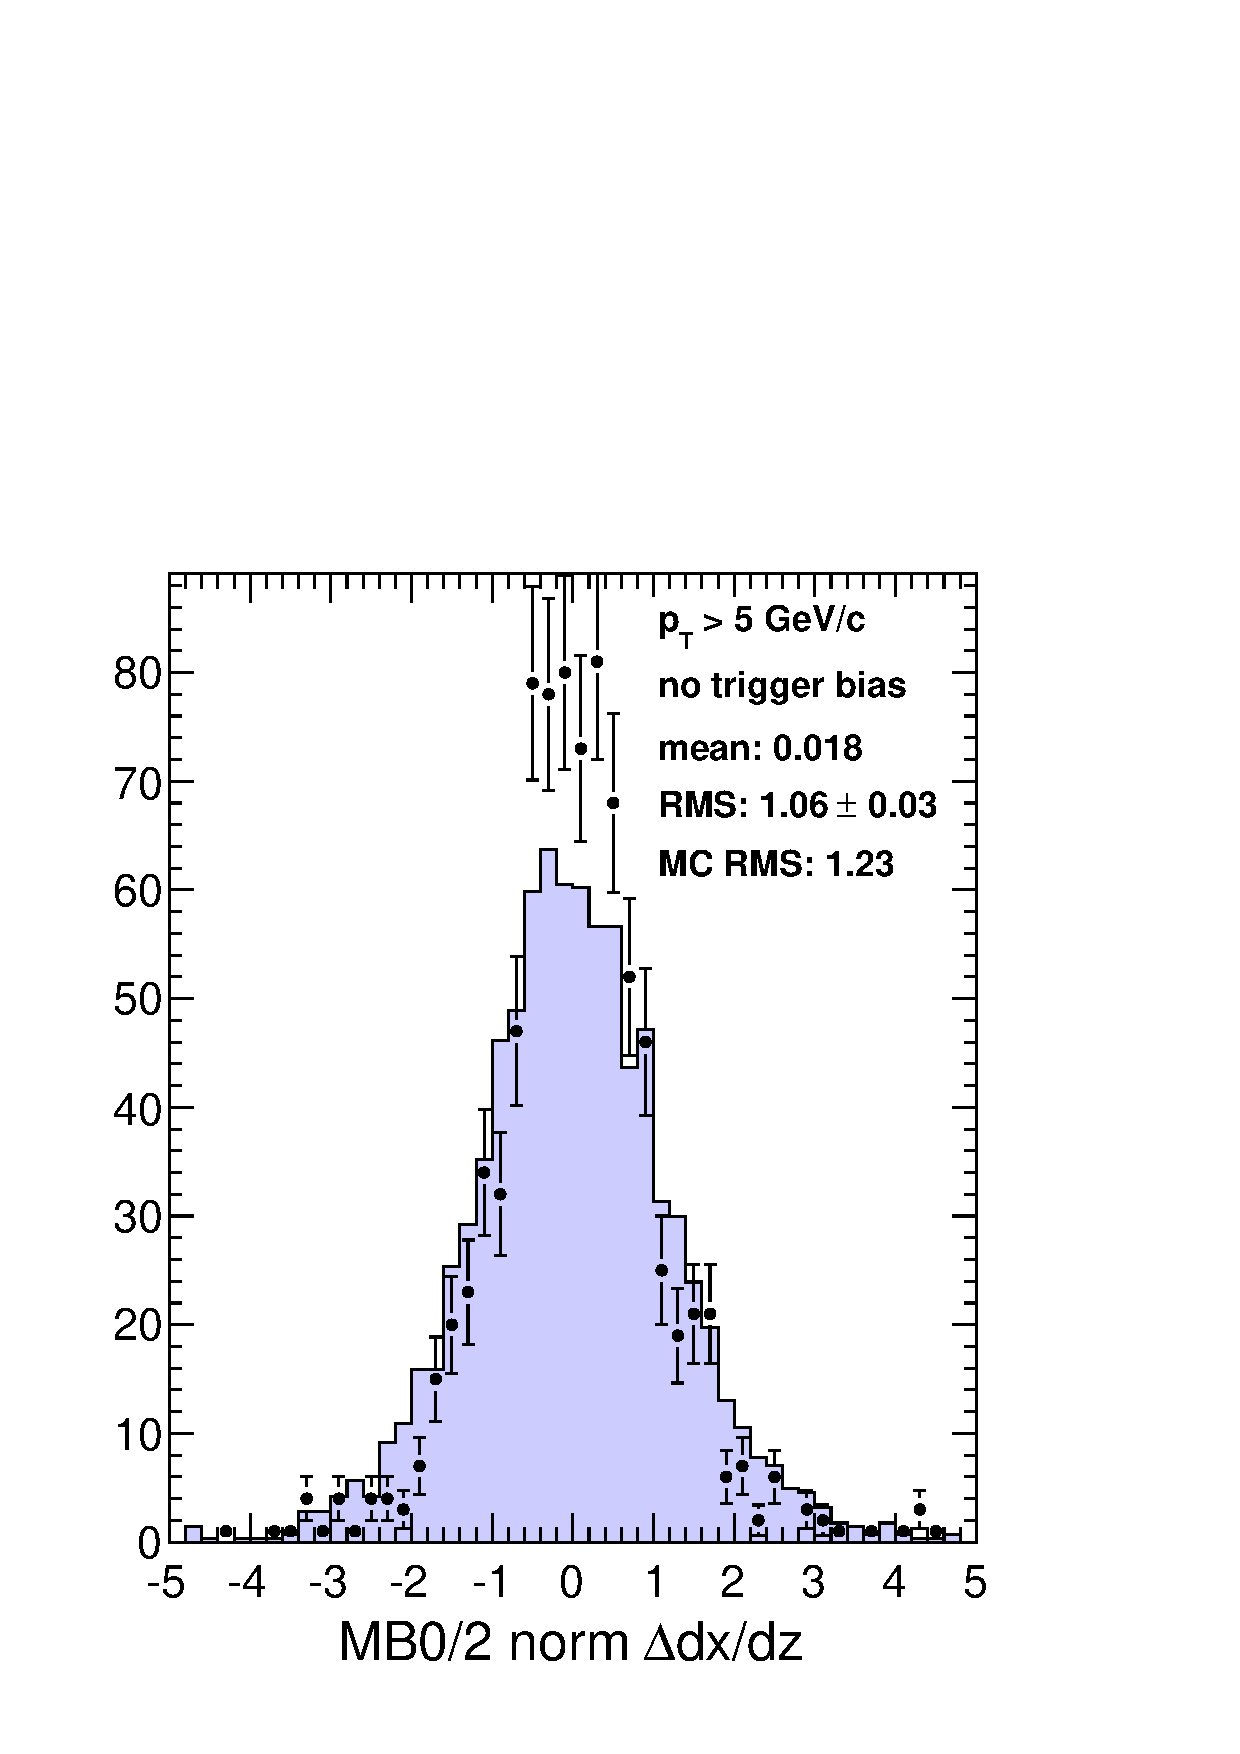
\includegraphics[width=0.24\linewidth]{mb02_dXdZnorm.pdf}
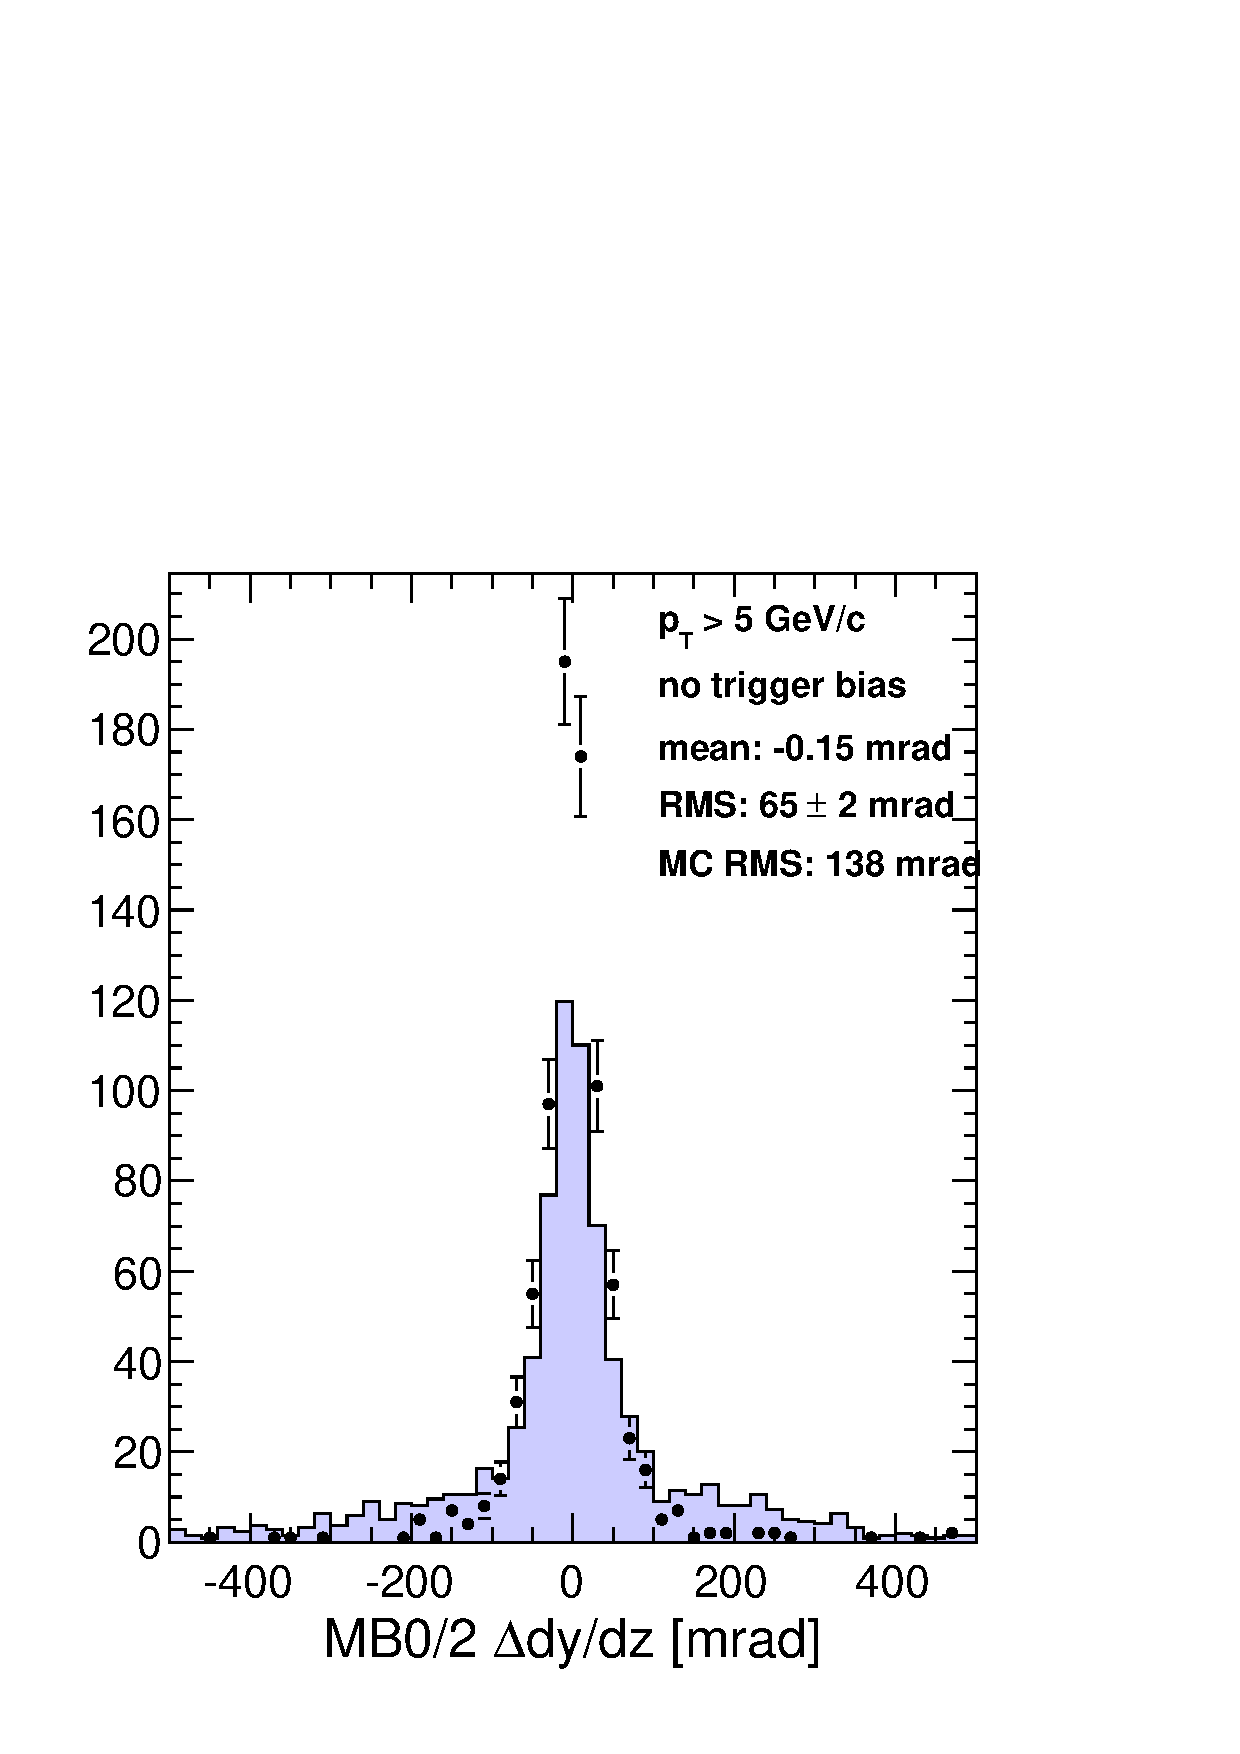
\includegraphics[width=0.24\linewidth]{mb02_dYdZ.pdf}
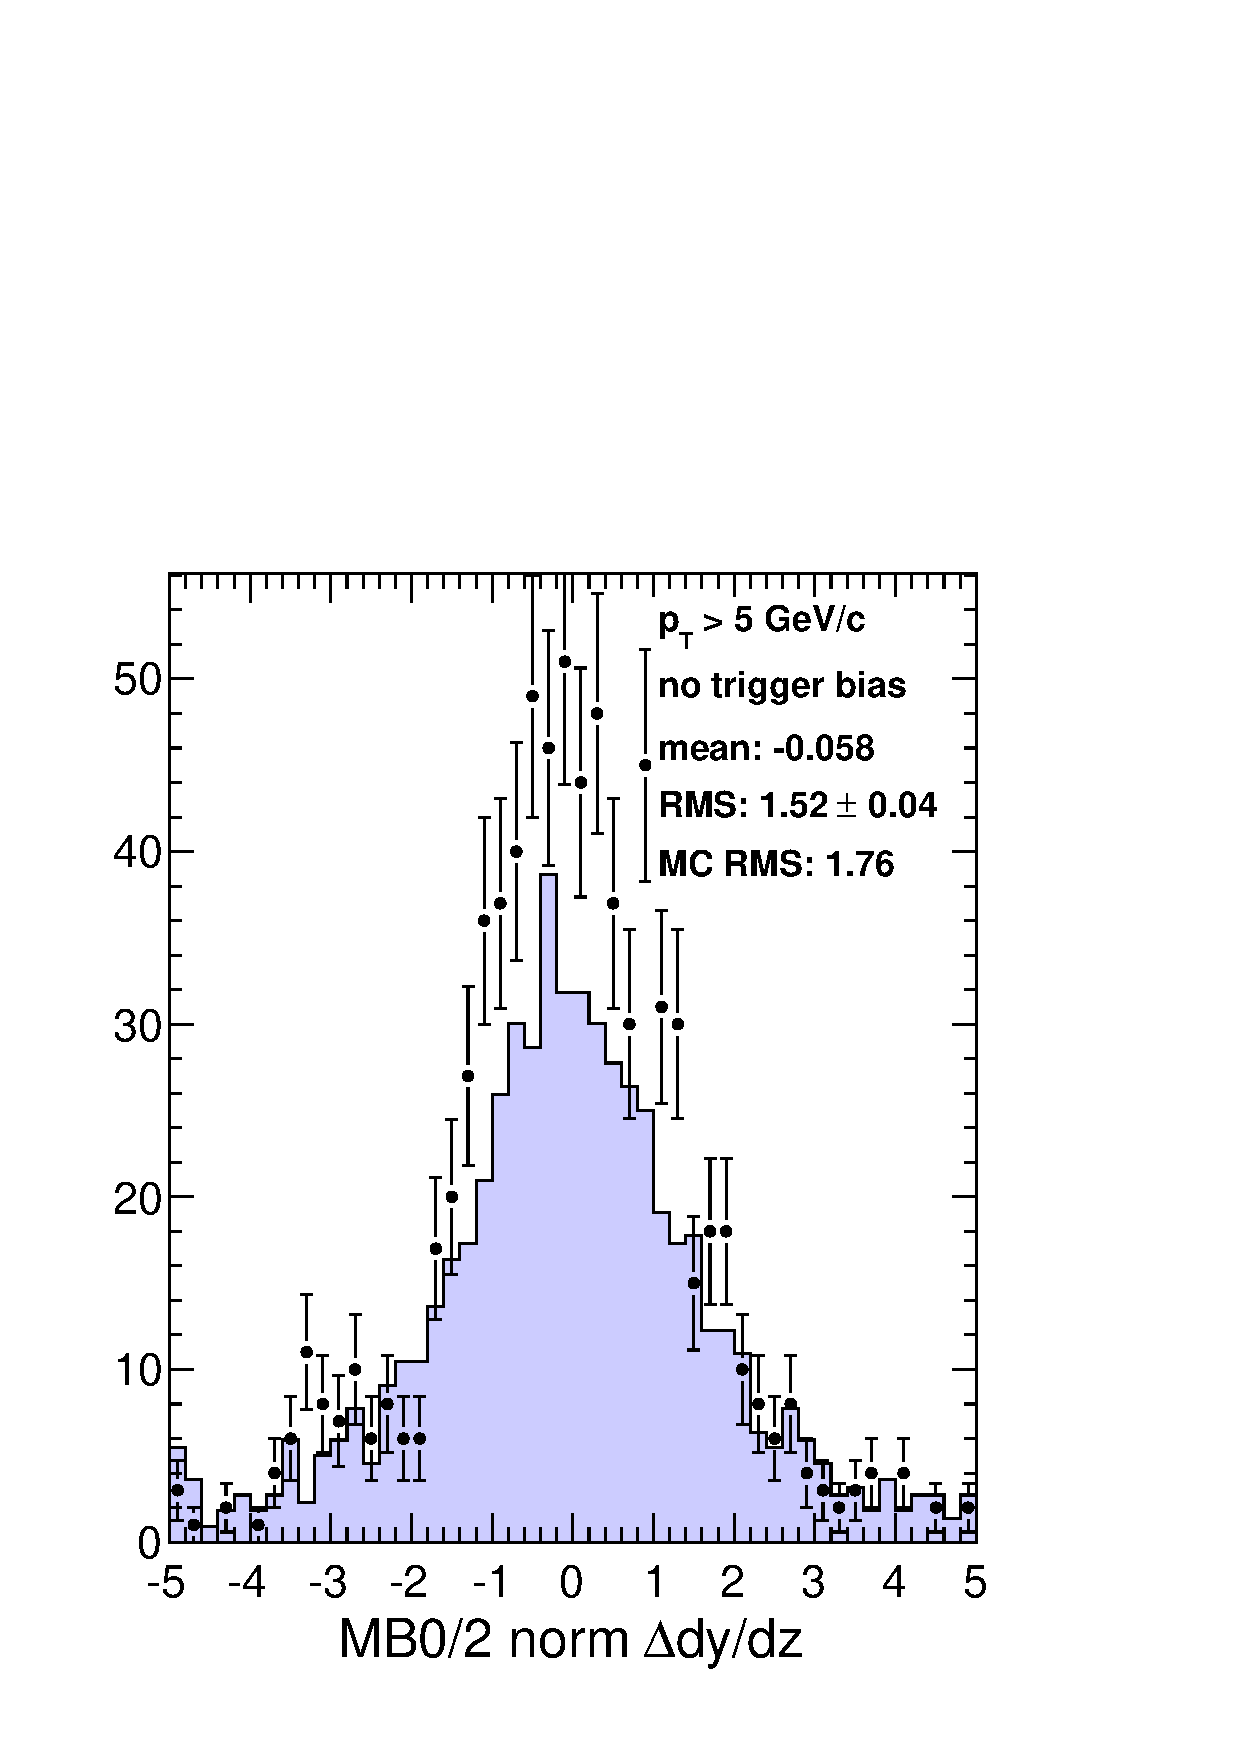
\includegraphics[width=0.24\linewidth]{mb02_dYdZnorm.pdf}
\end{frame}

\begin{frame}
\frametitle{MB0/3}

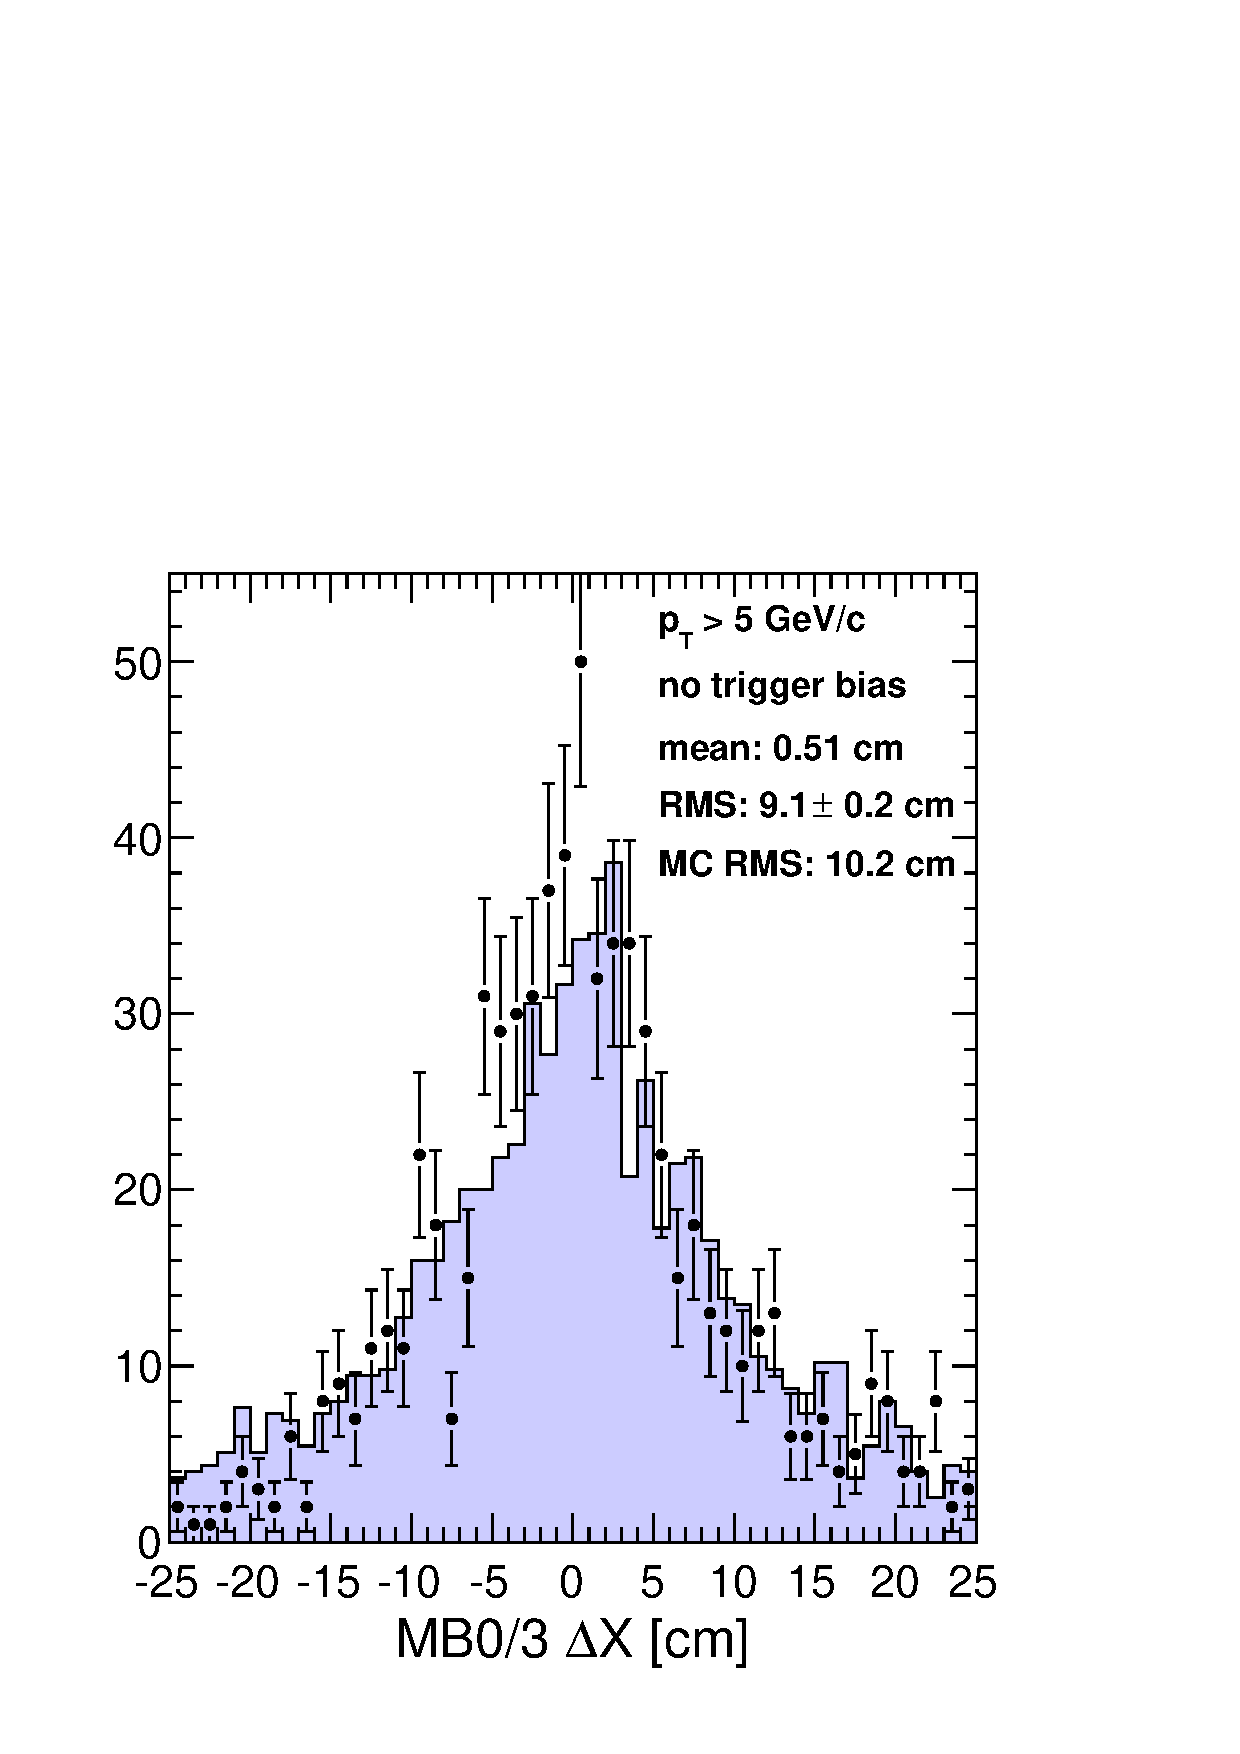
\includegraphics[width=0.24\linewidth]{mb03_X.pdf}
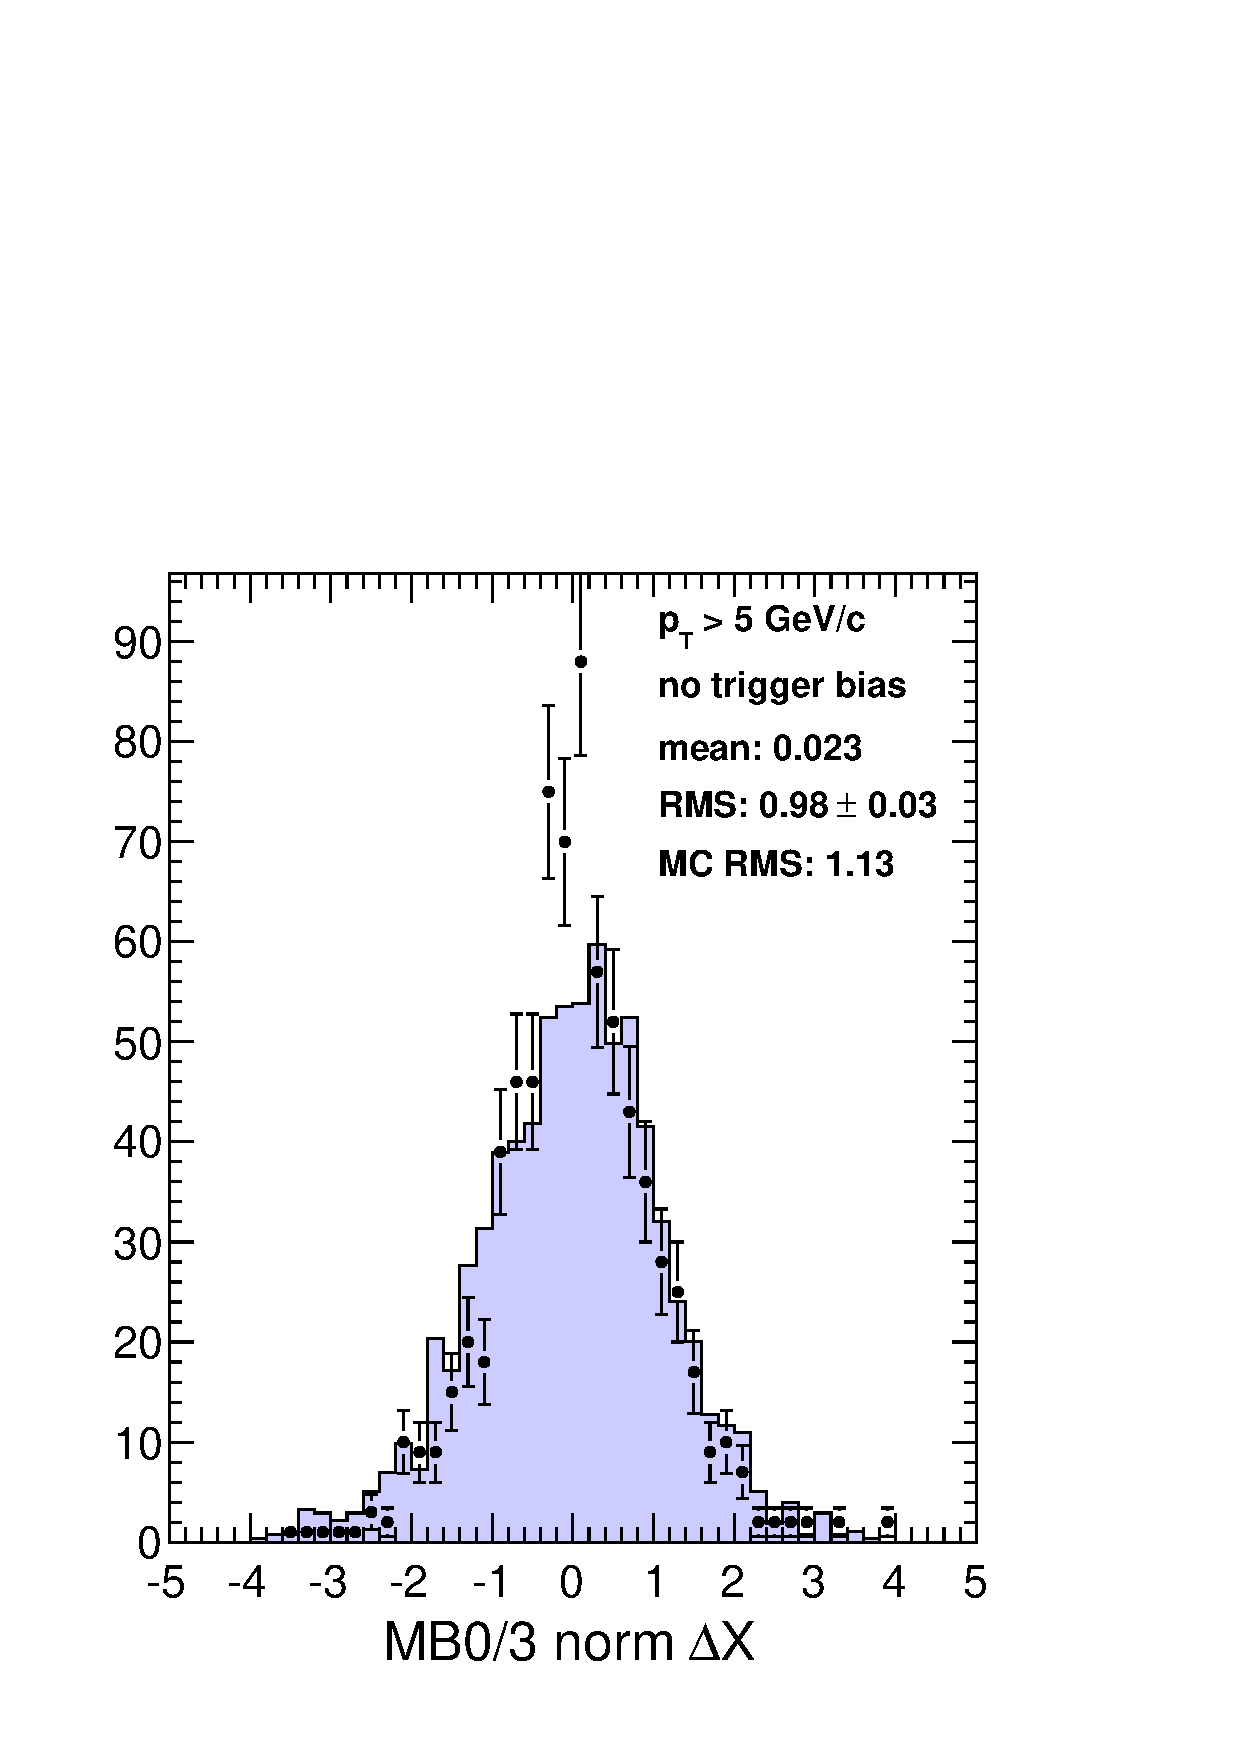
\includegraphics[width=0.24\linewidth]{mb03_Xnorm.pdf}
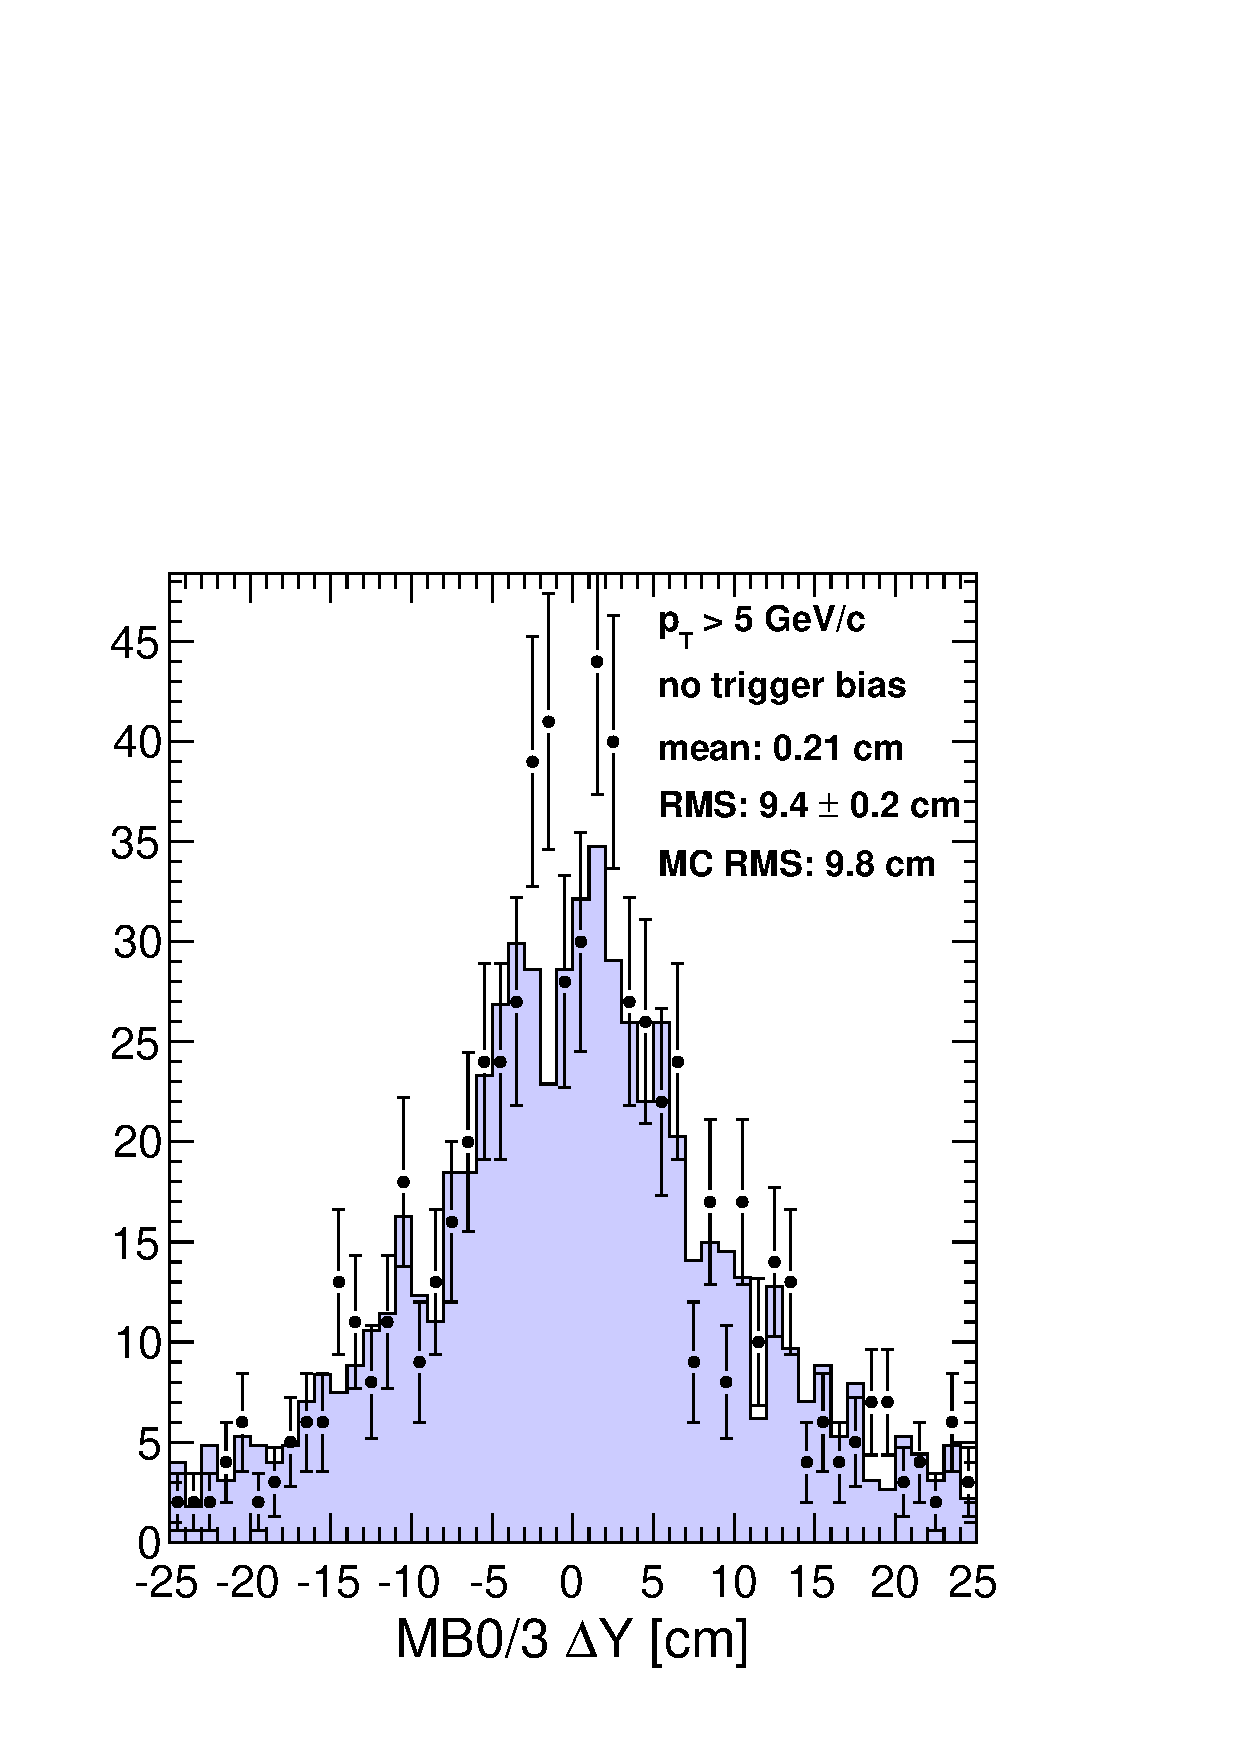
\includegraphics[width=0.24\linewidth]{mb03_Y.pdf}
\includegraphics[width=0.24\linewidth]{mb03_Ynorm.pdf}

\includegraphics[width=0.24\linewidth]{mb03_dXdZ.pdf}
\includegraphics[width=0.24\linewidth]{mb03_dXdZnorm.pdf}
\includegraphics[width=0.24\linewidth]{mb03_dYdZ.pdf}
\includegraphics[width=0.24\linewidth]{mb03_dYdZnorm.pdf}
\end{frame}

\begin{frame}
\frametitle{MB0/4}

\includegraphics[width=0.24\linewidth]{mb04_X.pdf}
\includegraphics[width=0.24\linewidth]{mb04_Xnorm.pdf}
\includegraphics[width=0.24\linewidth]{mb04_dXdZ.pdf}
\includegraphics[width=0.24\linewidth]{mb04_dXdZnorm.pdf}
\end{frame}

\begin{frame}
\frametitle{MB1/1}

\includegraphics[width=0.24\linewidth]{mb11_X.pdf}
\includegraphics[width=0.24\linewidth]{mb11_Xnorm.pdf}
\includegraphics[width=0.24\linewidth]{mb11_Y.pdf}
\includegraphics[width=0.24\linewidth]{mb11_Ynorm.pdf}

\includegraphics[width=0.24\linewidth]{mb11_dXdZ.pdf}
\includegraphics[width=0.24\linewidth]{mb11_dXdZnorm.pdf}
\includegraphics[width=0.24\linewidth]{mb11_dYdZ.pdf}
\includegraphics[width=0.24\linewidth]{mb11_dYdZnorm.pdf}
\end{frame}

\begin{frame}
\frametitle{MB1/2}

\includegraphics[width=0.24\linewidth]{mb12_X.pdf}
\includegraphics[width=0.24\linewidth]{mb12_Xnorm.pdf}
\includegraphics[width=0.24\linewidth]{mb12_Y.pdf}
\includegraphics[width=0.24\linewidth]{mb12_Ynorm.pdf}

\includegraphics[width=0.24\linewidth]{mb12_dXdZ.pdf}
\includegraphics[width=0.24\linewidth]{mb12_dXdZnorm.pdf}
\includegraphics[width=0.24\linewidth]{mb12_dYdZ.pdf}
\includegraphics[width=0.24\linewidth]{mb12_dYdZnorm.pdf}
\end{frame}

\begin{frame}
\frametitle{MB1/3}

\includegraphics[width=0.24\linewidth]{mb13_X.pdf}
\includegraphics[width=0.24\linewidth]{mb13_Xnorm.pdf}
\includegraphics[width=0.24\linewidth]{mb13_Y.pdf}
\includegraphics[width=0.24\linewidth]{mb13_Ynorm.pdf}

\includegraphics[width=0.24\linewidth]{mb13_dXdZ.pdf}
\includegraphics[width=0.24\linewidth]{mb13_dXdZnorm.pdf}
\includegraphics[width=0.24\linewidth]{mb13_dYdZ.pdf}
\includegraphics[width=0.24\linewidth]{mb13_dYdZnorm.pdf}
\end{frame}

\begin{frame}
\frametitle{MB1/4}

\includegraphics[width=0.24\linewidth]{mb14_X.pdf}
\includegraphics[width=0.24\linewidth]{mb14_Xnorm.pdf}
\includegraphics[width=0.24\linewidth]{mb14_dXdZ.pdf}
\includegraphics[width=0.24\linewidth]{mb14_dXdZnorm.pdf}
\end{frame}

\begin{frame}
\frametitle{MB2/1}

\includegraphics[width=0.24\linewidth]{mb21_X.pdf}
\includegraphics[width=0.24\linewidth]{mb21_Xnorm.pdf}
\includegraphics[width=0.24\linewidth]{mb21_Y.pdf}
\includegraphics[width=0.24\linewidth]{mb21_Ynorm.pdf}

\includegraphics[width=0.24\linewidth]{mb21_dXdZ.pdf}
\includegraphics[width=0.24\linewidth]{mb21_dXdZnorm.pdf}
\includegraphics[width=0.24\linewidth]{mb21_dYdZ.pdf}
\includegraphics[width=0.24\linewidth]{mb21_dYdZnorm.pdf}
\end{frame}

\begin{frame}
\frametitle{MB2/2}

\includegraphics[width=0.24\linewidth]{mb22_X.pdf}
\includegraphics[width=0.24\linewidth]{mb22_Xnorm.pdf}
\includegraphics[width=0.24\linewidth]{mb22_Y.pdf}
\includegraphics[width=0.24\linewidth]{mb22_Ynorm.pdf}

\includegraphics[width=0.24\linewidth]{mb22_dXdZ.pdf}
\includegraphics[width=0.24\linewidth]{mb22_dXdZnorm.pdf}
\includegraphics[width=0.24\linewidth]{mb22_dYdZ.pdf}
\includegraphics[width=0.24\linewidth]{mb22_dYdZnorm.pdf}
\end{frame}

\begin{frame}
\frametitle{MB2/3}

\includegraphics[width=0.24\linewidth]{mb23_X.pdf}
\includegraphics[width=0.24\linewidth]{mb23_Xnorm.pdf}
\includegraphics[width=0.24\linewidth]{mb23_Y.pdf}
\includegraphics[width=0.24\linewidth]{mb23_Ynorm.pdf}

\includegraphics[width=0.24\linewidth]{mb23_dXdZ.pdf}
\includegraphics[width=0.24\linewidth]{mb23_dXdZnorm.pdf}
\includegraphics[width=0.24\linewidth]{mb23_dYdZ.pdf}
\includegraphics[width=0.24\linewidth]{mb23_dYdZnorm.pdf}
\end{frame}

\begin{frame}
\frametitle{MB2/4}

\includegraphics[width=0.24\linewidth]{mb24_X.pdf}
\includegraphics[width=0.24\linewidth]{mb24_Xnorm.pdf}
\includegraphics[width=0.24\linewidth]{mb24_dXdZ.pdf}
\includegraphics[width=0.24\linewidth]{mb24_dXdZnorm.pdf}
\end{frame}

\begin{frame}
\frametitle{ME1/1}

\includegraphics[width=0.24\linewidth]{me11_X.pdf}
\includegraphics[width=0.24\linewidth]{me11_Xnorm.pdf}
\includegraphics[width=0.24\linewidth]{me11_Y.pdf}
\includegraphics[width=0.24\linewidth]{me11_Ynorm.pdf}

\includegraphics[width=0.24\linewidth]{me11_dXdZ.pdf}
\includegraphics[width=0.24\linewidth]{me11_dXdZnorm.pdf}
\includegraphics[width=0.24\linewidth]{me11_dYdZ.pdf}
\includegraphics[width=0.24\linewidth]{me11_dYdZnorm.pdf}
\end{frame}

\begin{frame}
\frametitle{ME1/2}

\includegraphics[width=0.24\linewidth]{me12_X.pdf}
\includegraphics[width=0.24\linewidth]{me12_Xnorm.pdf}
\includegraphics[width=0.24\linewidth]{me12_Y.pdf}
\includegraphics[width=0.24\linewidth]{me12_Ynorm.pdf}

\includegraphics[width=0.24\linewidth]{me12_dXdZ.pdf}
\includegraphics[width=0.24\linewidth]{me12_dXdZnorm.pdf}
\includegraphics[width=0.24\linewidth]{me12_dYdZ.pdf}
\includegraphics[width=0.24\linewidth]{me12_dYdZnorm.pdf}
\end{frame}

\begin{frame}
\frametitle{ME1/3}

\includegraphics[width=0.24\linewidth]{me13_X.pdf}
\includegraphics[width=0.24\linewidth]{me13_Xnorm.pdf}
\includegraphics[width=0.24\linewidth]{me13_Y.pdf}
\includegraphics[width=0.24\linewidth]{me13_Ynorm.pdf}

\includegraphics[width=0.24\linewidth]{me13_dXdZ.pdf}
\includegraphics[width=0.24\linewidth]{me13_dXdZnorm.pdf}
\includegraphics[width=0.24\linewidth]{me13_dYdZ.pdf}
\includegraphics[width=0.24\linewidth]{me13_dYdZnorm.pdf}
\end{frame}

\begin{frame}
\frametitle{ME2/1}

\includegraphics[width=0.24\linewidth]{me21_X.pdf}
\includegraphics[width=0.24\linewidth]{me21_Xnorm.pdf}
\includegraphics[width=0.24\linewidth]{me21_Y.pdf}
\includegraphics[width=0.24\linewidth]{me21_Ynorm.pdf}

\includegraphics[width=0.24\linewidth]{me21_dXdZ.pdf}
\includegraphics[width=0.24\linewidth]{me21_dXdZnorm.pdf}
\includegraphics[width=0.24\linewidth]{me21_dYdZ.pdf}
\includegraphics[width=0.24\linewidth]{me21_dYdZnorm.pdf}
\end{frame}

\begin{frame}
\frametitle{ME2/2}

\includegraphics[width=0.24\linewidth]{me22_X.pdf}
\includegraphics[width=0.24\linewidth]{me22_Xnorm.pdf}
\includegraphics[width=0.24\linewidth]{me22_Y.pdf}
\includegraphics[width=0.24\linewidth]{me22_Ynorm.pdf}

\includegraphics[width=0.24\linewidth]{me22_dXdZ.pdf}
\includegraphics[width=0.24\linewidth]{me22_dXdZnorm.pdf}
\includegraphics[width=0.24\linewidth]{me22_dYdZ.pdf}
\includegraphics[width=0.24\linewidth]{me22_dYdZnorm.pdf}
\end{frame}

\begin{frame}
\frametitle{ME3/1}

\includegraphics[width=0.24\linewidth]{me31_X.pdf}
\includegraphics[width=0.24\linewidth]{me31_Xnorm.pdf}
\includegraphics[width=0.24\linewidth]{me31_Y.pdf}
\includegraphics[width=0.24\linewidth]{me31_Ynorm.pdf}

\includegraphics[width=0.24\linewidth]{me31_dXdZ.pdf}
\includegraphics[width=0.24\linewidth]{me31_dXdZnorm.pdf}
\includegraphics[width=0.24\linewidth]{me31_dYdZ.pdf}
\includegraphics[width=0.24\linewidth]{me31_dYdZnorm.pdf}
\end{frame}

\begin{frame}
\frametitle{ME3/2}

\includegraphics[width=0.24\linewidth]{me32_X.pdf}
\includegraphics[width=0.24\linewidth]{me32_Xnorm.pdf}
\includegraphics[width=0.24\linewidth]{me32_Y.pdf}
\includegraphics[width=0.24\linewidth]{me32_Ynorm.pdf}

\includegraphics[width=0.24\linewidth]{me32_dXdZ.pdf}
\includegraphics[width=0.24\linewidth]{me32_dXdZnorm.pdf}
\includegraphics[width=0.24\linewidth]{me32_dYdZ.pdf}
\includegraphics[width=0.24\linewidth]{me32_dYdZnorm.pdf}
\end{frame}

\begin{frame}
\frametitle{ME4/1}

\includegraphics[width=0.24\linewidth]{me41_X.pdf}
\includegraphics[width=0.24\linewidth]{me41_Xnorm.pdf}
\includegraphics[width=0.24\linewidth]{me41_Y.pdf}
\includegraphics[width=0.24\linewidth]{me41_Ynorm.pdf}

\includegraphics[width=0.24\linewidth]{me41_dXdZ.pdf}
\includegraphics[width=0.24\linewidth]{me41_dXdZnorm.pdf}
\includegraphics[width=0.24\linewidth]{me41_dYdZ.pdf}
\includegraphics[width=0.24\linewidth]{me41_dYdZnorm.pdf}
\end{frame}

\begin{frame}
\frametitle{ME4/2}

\includegraphics[width=0.24\linewidth]{me42_X.pdf}
\includegraphics[width=0.24\linewidth]{me42_Xnorm.pdf}
\includegraphics[width=0.24\linewidth]{me42_Y.pdf}
\includegraphics[width=0.24\linewidth]{me42_Ynorm.pdf}

\includegraphics[width=0.24\linewidth]{me42_dXdZ.pdf}
\includegraphics[width=0.24\linewidth]{me42_dXdZnorm.pdf}
\includegraphics[width=0.24\linewidth]{me42_dYdZ.pdf}
\includegraphics[width=0.24\linewidth]{me42_dYdZnorm.pdf}
\end{frame}

\end{document}
